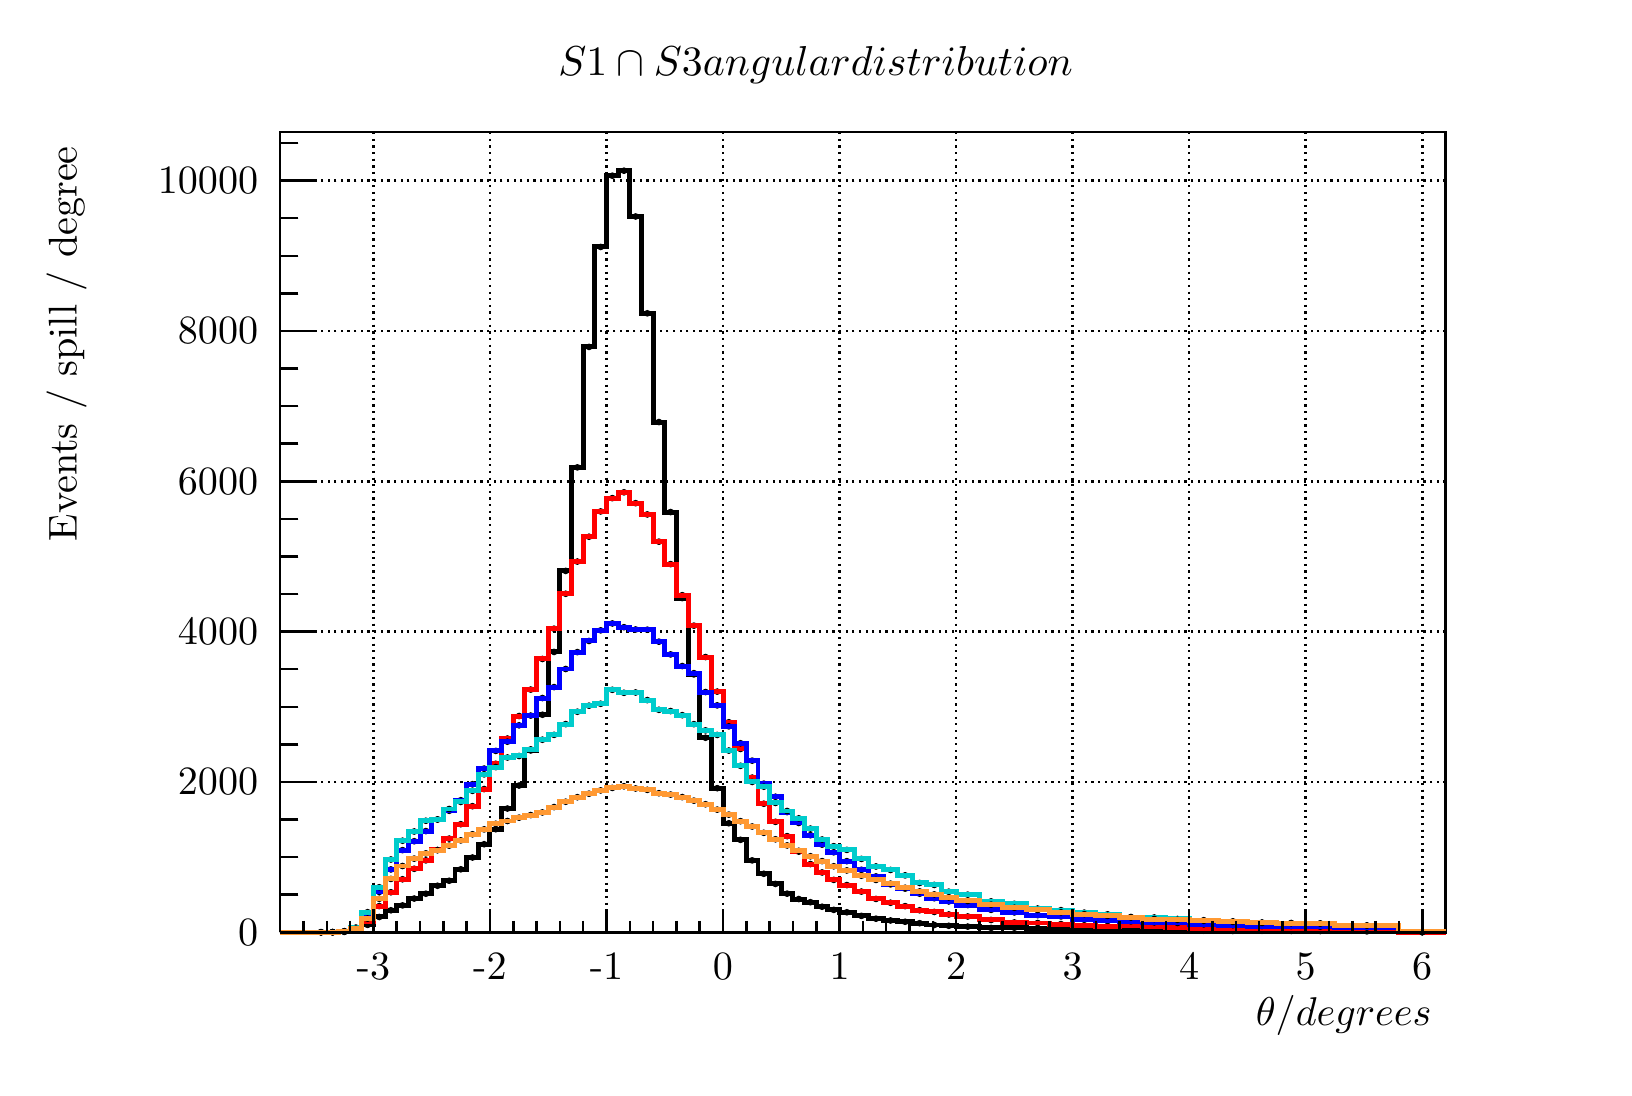
\begin{tikzpicture}
\pgfdeclareplotmark{cross} {
\pgfpathmoveto{\pgfpoint{-0.3\pgfplotmarksize}{\pgfplotmarksize}}
\pgfpathlineto{\pgfpoint{+0.3\pgfplotmarksize}{\pgfplotmarksize}}
\pgfpathlineto{\pgfpoint{+0.3\pgfplotmarksize}{0.3\pgfplotmarksize}}
\pgfpathlineto{\pgfpoint{+1\pgfplotmarksize}{0.3\pgfplotmarksize}}
\pgfpathlineto{\pgfpoint{+1\pgfplotmarksize}{-0.3\pgfplotmarksize}}
\pgfpathlineto{\pgfpoint{+0.3\pgfplotmarksize}{-0.3\pgfplotmarksize}}
\pgfpathlineto{\pgfpoint{+0.3\pgfplotmarksize}{-1.\pgfplotmarksize}}
\pgfpathlineto{\pgfpoint{-0.3\pgfplotmarksize}{-1.\pgfplotmarksize}}
\pgfpathlineto{\pgfpoint{-0.3\pgfplotmarksize}{-0.3\pgfplotmarksize}}
\pgfpathlineto{\pgfpoint{-1.\pgfplotmarksize}{-0.3\pgfplotmarksize}}
\pgfpathlineto{\pgfpoint{-1.\pgfplotmarksize}{0.3\pgfplotmarksize}}
\pgfpathlineto{\pgfpoint{-0.3\pgfplotmarksize}{0.3\pgfplotmarksize}}
\pgfpathclose
\pgfusepathqstroke
}
\pgfdeclareplotmark{cross*} {
\pgfpathmoveto{\pgfpoint{-0.3\pgfplotmarksize}{\pgfplotmarksize}}
\pgfpathlineto{\pgfpoint{+0.3\pgfplotmarksize}{\pgfplotmarksize}}
\pgfpathlineto{\pgfpoint{+0.3\pgfplotmarksize}{0.3\pgfplotmarksize}}
\pgfpathlineto{\pgfpoint{+1\pgfplotmarksize}{0.3\pgfplotmarksize}}
\pgfpathlineto{\pgfpoint{+1\pgfplotmarksize}{-0.3\pgfplotmarksize}}
\pgfpathlineto{\pgfpoint{+0.3\pgfplotmarksize}{-0.3\pgfplotmarksize}}
\pgfpathlineto{\pgfpoint{+0.3\pgfplotmarksize}{-1.\pgfplotmarksize}}
\pgfpathlineto{\pgfpoint{-0.3\pgfplotmarksize}{-1.\pgfplotmarksize}}
\pgfpathlineto{\pgfpoint{-0.3\pgfplotmarksize}{-0.3\pgfplotmarksize}}
\pgfpathlineto{\pgfpoint{-1.\pgfplotmarksize}{-0.3\pgfplotmarksize}}
\pgfpathlineto{\pgfpoint{-1.\pgfplotmarksize}{0.3\pgfplotmarksize}}
\pgfpathlineto{\pgfpoint{-0.3\pgfplotmarksize}{0.3\pgfplotmarksize}}
\pgfpathclose
\pgfusepathqfillstroke
}
\pgfdeclareplotmark{newstar} {
\pgfpathmoveto{\pgfqpoint{0pt}{\pgfplotmarksize}}
\pgfpathlineto{\pgfqpointpolar{44}{0.5\pgfplotmarksize}}
\pgfpathlineto{\pgfqpointpolar{18}{\pgfplotmarksize}}
\pgfpathlineto{\pgfqpointpolar{-20}{0.5\pgfplotmarksize}}
\pgfpathlineto{\pgfqpointpolar{-54}{\pgfplotmarksize}}
\pgfpathlineto{\pgfqpointpolar{-90}{0.5\pgfplotmarksize}}
\pgfpathlineto{\pgfqpointpolar{234}{\pgfplotmarksize}}
\pgfpathlineto{\pgfqpointpolar{198}{0.5\pgfplotmarksize}}
\pgfpathlineto{\pgfqpointpolar{162}{\pgfplotmarksize}}
\pgfpathlineto{\pgfqpointpolar{134}{0.5\pgfplotmarksize}}
\pgfpathclose
\pgfusepathqstroke
}
\pgfdeclareplotmark{newstar*} {
\pgfpathmoveto{\pgfqpoint{0pt}{\pgfplotmarksize}}
\pgfpathlineto{\pgfqpointpolar{44}{0.5\pgfplotmarksize}}
\pgfpathlineto{\pgfqpointpolar{18}{\pgfplotmarksize}}
\pgfpathlineto{\pgfqpointpolar{-20}{0.5\pgfplotmarksize}}
\pgfpathlineto{\pgfqpointpolar{-54}{\pgfplotmarksize}}
\pgfpathlineto{\pgfqpointpolar{-90}{0.5\pgfplotmarksize}}
\pgfpathlineto{\pgfqpointpolar{234}{\pgfplotmarksize}}
\pgfpathlineto{\pgfqpointpolar{198}{0.5\pgfplotmarksize}}
\pgfpathlineto{\pgfqpointpolar{162}{\pgfplotmarksize}}
\pgfpathlineto{\pgfqpointpolar{134}{0.5\pgfplotmarksize}}
\pgfpathclose
\pgfusepathqfillstroke
}
\definecolor{c}{rgb}{1,1,1};
\draw [color=c, fill=c] (0,0) rectangle (20,13.1973);
\draw [color=c, fill=c] (3.2,1.71565) rectangle (18,11.8776);
\definecolor{c}{rgb}{0,0,0};
\draw [c,line width=0.9] (3.2,1.71565) -- (3.2,11.8776) -- (18,11.8776) -- (18,1.71565) -- (3.2,1.71565);
\definecolor{c}{rgb}{1,1,1};
\draw [color=c, fill=c] (3.2,1.71565) rectangle (18,11.8776);
\definecolor{c}{rgb}{0,0,0};
\draw [c,line width=0.9] (3.2,1.71565) -- (3.2,11.8776) -- (18,11.8776) -- (18,1.71565) -- (3.2,1.71565);
\draw [c,line width=0.9] (3.2,1.71565) -- (18,1.71565);
\draw [c,dash pattern=on 0.80pt off 1.60pt ,line width=0.9] (4.384,11.8776) -- (4.384,1.71565);
\draw [c,dash pattern=on 0.80pt off 1.60pt ,line width=0.9] (5.864,11.8776) -- (5.864,1.71565);
\draw [c,dash pattern=on 0.80pt off 1.60pt ,line width=0.9] (7.344,11.8776) -- (7.344,1.71565);
\draw [c,dash pattern=on 0.80pt off 1.60pt ,line width=0.9] (8.824,11.8776) -- (8.824,1.71565);
\draw [c,dash pattern=on 0.80pt off 1.60pt ,line width=0.9] (10.304,11.8776) -- (10.304,1.71565);
\draw [c,dash pattern=on 0.80pt off 1.60pt ,line width=0.9] (11.784,11.8776) -- (11.784,1.71565);
\draw [c,dash pattern=on 0.80pt off 1.60pt ,line width=0.9] (13.264,11.8776) -- (13.264,1.71565);
\draw [c,dash pattern=on 0.80pt off 1.60pt ,line width=0.9] (14.744,11.8776) -- (14.744,1.71565);
\draw [c,dash pattern=on 0.80pt off 1.60pt ,line width=0.9] (16.224,11.8776) -- (16.224,1.71565);
\draw [c,dash pattern=on 0.80pt off 1.60pt ,line width=0.9] (17.704,11.8776) -- (17.704,1.71565);
\draw [c,dash pattern=on 0.80pt off 1.60pt ,line width=0.9] (4.384,11.8776) -- (4.384,1.71565);
\draw [c,dash pattern=on 0.80pt off 1.60pt ,line width=0.9] (17.704,11.8776) -- (17.704,1.71565);
\draw [c,line width=0.9] (3.2,1.71565) -- (3.2,11.8776);
\draw [c,dash pattern=on 0.80pt off 1.60pt ,line width=0.9] (18,1.71565) -- (3.2,1.71565);
\draw [c,dash pattern=on 0.80pt off 1.60pt ,line width=0.9] (18,3.62476) -- (3.2,3.62476);
\draw [c,dash pattern=on 0.80pt off 1.60pt ,line width=0.9] (18,5.53388) -- (3.2,5.53388);
\draw [c,dash pattern=on 0.80pt off 1.60pt ,line width=0.9] (18,7.443) -- (3.2,7.443);
\draw [c,dash pattern=on 0.80pt off 1.60pt ,line width=0.9] (18,9.35212) -- (3.2,9.35212);
\draw [c,dash pattern=on 0.80pt off 1.60pt ,line width=0.9] (18,11.2612) -- (3.2,11.2612);
\draw [c,dash pattern=on 0.80pt off 1.60pt ,line width=0.9] (18,11.2612) -- (3.2,11.2612);
\definecolor{c}{rgb}{0,0,0.6};
\draw [c,line width=0.9] (3.2,1.71565) -- (3.348,1.71565) -- (3.348,1.71565) -- (3.496,1.71565) -- (3.496,1.71565) -- (3.644,1.71565) -- (3.644,1.71565) -- (3.792,1.71565) -- (3.792,1.71565) -- (3.94,1.71565) -- (3.94,1.71565) -- (4.088,1.71565) --
 (4.088,1.71565) -- (4.236,1.71565) -- (4.236,1.71565) -- (4.384,1.71565) -- (4.384,1.71565) -- (4.532,1.71565) -- (4.532,1.71565) -- (4.68,1.71565) -- (4.68,1.71565) -- (4.828,1.71565) -- (4.828,1.71565) -- (4.976,1.71565) -- (4.976,1.71565) --
 (5.124,1.71565) -- (5.124,1.71565) -- (5.272,1.71565) -- (5.272,1.71565) -- (5.42,1.71565) -- (5.42,1.71565) -- (5.568,1.71565) -- (5.568,1.71565) -- (5.716,1.71565) -- (5.716,1.71565) -- (5.864,1.71565) -- (5.864,1.71565) -- (6.012,1.71565) --
 (6.012,1.71565) -- (6.16,1.71565) -- (6.16,1.71565) -- (6.308,1.71565) -- (6.308,1.71565) -- (6.456,1.71565) -- (6.456,1.71565) -- (6.604,1.71565) -- (6.604,1.71565) -- (6.752,1.71565) -- (6.752,1.71565) -- (6.9,1.71565) -- (6.9,1.71565) --
 (7.048,1.71565) -- (7.048,1.71565) -- (7.196,1.71565) -- (7.196,1.71565) -- (7.344,1.71565) -- (7.344,1.71565) -- (7.492,1.71565) -- (7.492,1.71565) -- (7.64,1.71565) -- (7.64,1.71565) -- (7.788,1.71565) -- (7.788,1.71565) -- (7.936,1.71565) --
 (7.936,1.71565) -- (8.084,1.71565) -- (8.084,1.71565) -- (8.232,1.71565) -- (8.232,1.71565) -- (8.38,1.71565) -- (8.38,1.71565) -- (8.528,1.71565) -- (8.528,1.71565) -- (8.676,1.71565) -- (8.676,1.71565) -- (8.824,1.71565) -- (8.824,1.71565) --
 (8.972,1.71565) -- (8.972,1.71565) -- (9.12,1.71565) -- (9.12,1.71565) -- (9.268,1.71565) -- (9.268,1.71565) -- (9.416,1.71565) -- (9.416,1.71565) -- (9.564,1.71565) -- (9.564,1.71565) -- (9.712,1.71565) -- (9.712,1.71565) -- (9.86,1.71565) --
 (9.86,1.71565) -- (10.008,1.71565) -- (10.008,1.71565) -- (10.156,1.71565) -- (10.156,1.71565) -- (10.304,1.71565) -- (10.304,1.71565) -- (10.489,1.71565) -- (10.489,1.71565) -- (10.674,1.71565) -- (10.674,1.71565) -- (10.859,1.71565) --
 (10.859,1.71565) -- (11.044,1.71565) -- (11.044,1.71565) -- (11.229,1.71565) -- (11.229,1.71565) -- (11.414,1.71565) -- (11.414,1.71565) -- (11.599,1.71565) -- (11.599,1.71565) -- (11.784,1.71565) -- (11.784,1.71565) -- (12.08,1.71565) --
 (12.08,1.71565) -- (12.376,1.71565) -- (12.376,1.71565) -- (12.672,1.71565) -- (12.672,1.71565) -- (12.968,1.71565) -- (12.968,1.71565) -- (13.264,1.71565) -- (13.264,1.71565) -- (13.56,1.71565) -- (13.56,1.71565) -- (13.856,1.71565) --
 (13.856,1.71565) -- (14.152,1.71565) -- (14.152,1.71565) -- (14.448,1.71565) -- (14.448,1.71565) -- (14.744,1.71565) -- (14.744,1.71565) -- (15.114,1.71565) -- (15.114,1.71565) -- (15.484,1.71565) -- (15.484,1.71565) -- (15.854,1.71565) --
 (15.854,1.71565) -- (16.224,1.71565) -- (16.224,1.71565) -- (16.594,1.71565) -- (16.594,1.71565) -- (17.408,1.71565) -- (17.408,1.71565) -- (18,1.71565);
\definecolor{c}{rgb}{0,0,0};
\draw [c,line width=0.9] (3.2,1.71565) -- (18,1.71565);
\draw [c,line width=0.9] (4.384,2.00863) -- (4.384,1.71565);
\draw [c,line width=0.9] (4.68,1.86214) -- (4.68,1.71565);
\draw [c,line width=0.9] (4.976,1.86214) -- (4.976,1.71565);
\draw [c,line width=0.9] (5.272,1.86214) -- (5.272,1.71565);
\draw [c,line width=0.9] (5.568,1.86214) -- (5.568,1.71565);
\draw [c,line width=0.9] (5.864,2.00863) -- (5.864,1.71565);
\draw [c,line width=0.9] (6.16,1.86214) -- (6.16,1.71565);
\draw [c,line width=0.9] (6.456,1.86214) -- (6.456,1.71565);
\draw [c,line width=0.9] (6.752,1.86214) -- (6.752,1.71565);
\draw [c,line width=0.9] (7.048,1.86214) -- (7.048,1.71565);
\draw [c,line width=0.9] (7.344,2.00863) -- (7.344,1.71565);
\draw [c,line width=0.9] (7.64,1.86214) -- (7.64,1.71565);
\draw [c,line width=0.9] (7.936,1.86214) -- (7.936,1.71565);
\draw [c,line width=0.9] (8.232,1.86214) -- (8.232,1.71565);
\draw [c,line width=0.9] (8.528,1.86214) -- (8.528,1.71565);
\draw [c,line width=0.9] (8.824,2.00863) -- (8.824,1.71565);
\draw [c,line width=0.9] (9.12,1.86214) -- (9.12,1.71565);
\draw [c,line width=0.9] (9.416,1.86214) -- (9.416,1.71565);
\draw [c,line width=0.9] (9.712,1.86214) -- (9.712,1.71565);
\draw [c,line width=0.9] (10.008,1.86214) -- (10.008,1.71565);
\draw [c,line width=0.9] (10.304,2.00863) -- (10.304,1.71565);
\draw [c,line width=0.9] (10.6,1.86214) -- (10.6,1.71565);
\draw [c,line width=0.9] (10.896,1.86214) -- (10.896,1.71565);
\draw [c,line width=0.9] (11.192,1.86214) -- (11.192,1.71565);
\draw [c,line width=0.9] (11.488,1.86214) -- (11.488,1.71565);
\draw [c,line width=0.9] (11.784,2.00863) -- (11.784,1.71565);
\draw [c,line width=0.9] (12.08,1.86214) -- (12.08,1.71565);
\draw [c,line width=0.9] (12.376,1.86214) -- (12.376,1.71565);
\draw [c,line width=0.9] (12.672,1.86214) -- (12.672,1.71565);
\draw [c,line width=0.9] (12.968,1.86214) -- (12.968,1.71565);
\draw [c,line width=0.9] (13.264,2.00863) -- (13.264,1.71565);
\draw [c,line width=0.9] (13.56,1.86214) -- (13.56,1.71565);
\draw [c,line width=0.9] (13.856,1.86214) -- (13.856,1.71565);
\draw [c,line width=0.9] (14.152,1.86214) -- (14.152,1.71565);
\draw [c,line width=0.9] (14.448,1.86214) -- (14.448,1.71565);
\draw [c,line width=0.9] (14.744,2.00863) -- (14.744,1.71565);
\draw [c,line width=0.9] (15.04,1.86214) -- (15.04,1.71565);
\draw [c,line width=0.9] (15.336,1.86214) -- (15.336,1.71565);
\draw [c,line width=0.9] (15.632,1.86214) -- (15.632,1.71565);
\draw [c,line width=0.9] (15.928,1.86214) -- (15.928,1.71565);
\draw [c,line width=0.9] (16.224,2.00863) -- (16.224,1.71565);
\draw [c,line width=0.9] (16.52,1.86214) -- (16.52,1.71565);
\draw [c,line width=0.9] (16.816,1.86214) -- (16.816,1.71565);
\draw [c,line width=0.9] (17.112,1.86214) -- (17.112,1.71565);
\draw [c,line width=0.9] (17.408,1.86214) -- (17.408,1.71565);
\draw [c,line width=0.9] (17.704,2.00863) -- (17.704,1.71565);
\draw [c,line width=0.9] (4.384,2.00863) -- (4.384,1.71565);
\draw [c,line width=0.9] (4.088,1.86214) -- (4.088,1.71565);
\draw [c,line width=0.9] (3.792,1.86214) -- (3.792,1.71565);
\draw [c,line width=0.9] (3.496,1.86214) -- (3.496,1.71565);
\draw [c,line width=0.9] (17.704,2.00863) -- (17.704,1.71565);
\draw [anchor=base] (4.384,1.12177) node[scale=1.45043, color=c, rotate=0]{-3};
\draw [anchor=base] (5.864,1.12177) node[scale=1.45043, color=c, rotate=0]{-2};
\draw [anchor=base] (7.344,1.12177) node[scale=1.45043, color=c, rotate=0]{-1};
\draw [anchor=base] (8.824,1.12177) node[scale=1.45043, color=c, rotate=0]{0};
\draw [anchor=base] (10.304,1.12177) node[scale=1.45043, color=c, rotate=0]{1};
\draw [anchor=base] (11.784,1.12177) node[scale=1.45043, color=c, rotate=0]{2};
\draw [anchor=base] (13.264,1.12177) node[scale=1.45043, color=c, rotate=0]{3};
\draw [anchor=base] (14.744,1.12177) node[scale=1.45043, color=c, rotate=0]{4};
\draw [anchor=base] (16.224,1.12177) node[scale=1.45043, color=c, rotate=0]{5};
\draw [anchor=base] (17.704,1.12177) node[scale=1.45043, color=c, rotate=0]{6};
\draw [anchor= east] (18,0.659864) node[scale=1.45043, color=c, rotate=0]{$ \theta / degrees$};
\draw [c,line width=0.9] (3.2,1.71565) -- (3.2,11.8776);
\draw [c,line width=0.9] (3.662,1.71565) -- (3.2,1.71565);
\draw [c,line width=0.9] (3.431,2.19293) -- (3.2,2.19293);
\draw [c,line width=0.9] (3.431,2.67021) -- (3.2,2.67021);
\draw [c,line width=0.9] (3.431,3.14748) -- (3.2,3.14748);
\draw [c,line width=0.9] (3.662,3.62476) -- (3.2,3.62476);
\draw [c,line width=0.9] (3.431,4.10204) -- (3.2,4.10204);
\draw [c,line width=0.9] (3.431,4.57932) -- (3.2,4.57932);
\draw [c,line width=0.9] (3.431,5.0566) -- (3.2,5.0566);
\draw [c,line width=0.9] (3.662,5.53388) -- (3.2,5.53388);
\draw [c,line width=0.9] (3.431,6.01116) -- (3.2,6.01116);
\draw [c,line width=0.9] (3.431,6.48844) -- (3.2,6.48844);
\draw [c,line width=0.9] (3.431,6.96572) -- (3.2,6.96572);
\draw [c,line width=0.9] (3.662,7.443) -- (3.2,7.443);
\draw [c,line width=0.9] (3.431,7.92028) -- (3.2,7.92028);
\draw [c,line width=0.9] (3.431,8.39756) -- (3.2,8.39756);
\draw [c,line width=0.9] (3.431,8.87484) -- (3.2,8.87484);
\draw [c,line width=0.9] (3.662,9.35212) -- (3.2,9.35212);
\draw [c,line width=0.9] (3.431,9.8294) -- (3.2,9.8294);
\draw [c,line width=0.9] (3.431,10.3067) -- (3.2,10.3067);
\draw [c,line width=0.9] (3.431,10.784) -- (3.2,10.784);
\draw [c,line width=0.9] (3.662,11.2612) -- (3.2,11.2612);
\draw [c,line width=0.9] (3.662,11.2612) -- (3.2,11.2612);
\draw [c,line width=0.9] (3.431,11.7385) -- (3.2,11.7385);
\draw [anchor= east] (3.1,1.71565) node[scale=1.45043, color=c, rotate=0]{0};
\draw [anchor= east] (3.1,3.62476) node[scale=1.45043, color=c, rotate=0]{2000};
\draw [anchor= east] (3.1,5.53388) node[scale=1.45043, color=c, rotate=0]{4000};
\draw [anchor= east] (3.1,7.443) node[scale=1.45043, color=c, rotate=0]{6000};
\draw [anchor= east] (3.1,9.35212) node[scale=1.45043, color=c, rotate=0]{8000};
\draw [anchor= east] (3.1,11.2612) node[scale=1.45043, color=c, rotate=0]{10000};
\draw [anchor= east] (0.485714,11.8776) node[scale=1.45043, color=c, rotate=90]{ Events / spill / degree};
\draw [c,line width=1.8] (3.866,1.71595) -- (3.866,1.71598);
\draw [c,line width=1.8] (3.866,1.71598) -- (3.866,1.71602);
\foreach \P in {(3.866,1.71598)}{\draw[mark options={color=c,fill=c},mark size=2.402402pt,mark=*,mark size=1pt] plot coordinates {\P};}
\draw [c,line width=1.8] (4.014,1.72602) -- (4.014,1.72622);
\draw [c,line width=1.8] (4.014,1.72622) -- (4.014,1.72642);
\foreach \P in {(4.014,1.72622)}{\draw[mark options={color=c,fill=c},mark size=2.402402pt,mark=*,mark size=1pt] plot coordinates {\P};}
\draw [c,line width=1.8] (4.162,1.74717) -- (4.162,1.74753);
\draw [c,line width=1.8] (4.162,1.74753) -- (4.162,1.74788);
\foreach \P in {(4.162,1.74753)}{\draw[mark options={color=c,fill=c},mark size=2.402402pt,mark=*,mark size=1pt] plot coordinates {\P};}
\draw [c,line width=1.8] (4.31,1.80928) -- (4.31,1.80989);
\draw [c,line width=1.8] (4.31,1.80989) -- (4.31,1.81049);
\foreach \P in {(4.31,1.80989)}{\draw[mark options={color=c,fill=c},mark size=2.402402pt,mark=*,mark size=1pt] plot coordinates {\P};}
\draw [c,line width=1.8] (4.458,1.90916) -- (4.458,1.91003);
\draw [c,line width=1.8] (4.458,1.91003) -- (4.458,1.91089);
\foreach \P in {(4.458,1.91003)}{\draw[mark options={color=c,fill=c},mark size=2.402402pt,mark=*,mark size=1pt] plot coordinates {\P};}
\draw [c,line width=1.8] (4.606,1.99401) -- (4.606,1.99505);
\draw [c,line width=1.8] (4.606,1.99505) -- (4.606,1.99608);
\foreach \P in {(4.606,1.99505)}{\draw[mark options={color=c,fill=c},mark size=2.402402pt,mark=*,mark size=1pt] plot coordinates {\P};}
\draw [c,line width=1.8] (4.754,2.05623) -- (4.754,2.05738);
\draw [c,line width=1.8] (4.754,2.05738) -- (4.754,2.05852);
\foreach \P in {(4.754,2.05738)}{\draw[mark options={color=c,fill=c},mark size=2.402402pt,mark=*,mark size=1pt] plot coordinates {\P};}
\draw [c,line width=1.8] (4.902,2.14291) -- (4.902,2.1442);
\draw [c,line width=1.8] (4.902,2.1442) -- (4.902,2.14548);
\foreach \P in {(4.902,2.1442)}{\draw[mark options={color=c,fill=c},mark size=2.402402pt,mark=*,mark size=1pt] plot coordinates {\P};}
\draw [c,line width=1.8] (5.05,2.20396) -- (5.05,2.20534);
\draw [c,line width=1.8] (5.05,2.20534) -- (5.05,2.20671);
\foreach \P in {(5.05,2.20534)}{\draw[mark options={color=c,fill=c},mark size=2.402402pt,mark=*,mark size=1pt] plot coordinates {\P};}
\draw [c,line width=1.8] (5.198,2.30504) -- (5.198,2.30655);
\draw [c,line width=1.8] (5.198,2.30655) -- (5.198,2.30806);
\foreach \P in {(5.198,2.30655)}{\draw[mark options={color=c,fill=c},mark size=2.402402pt,mark=*,mark size=1pt] plot coordinates {\P};}
\draw [c,line width=1.8] (5.346,2.36846) -- (5.346,2.37004);
\draw [c,line width=1.8] (5.346,2.37004) -- (5.346,2.37162);
\foreach \P in {(5.346,2.37004)}{\draw[mark options={color=c,fill=c},mark size=2.402402pt,mark=*,mark size=1pt] plot coordinates {\P};}
\draw [c,line width=1.8] (5.494,2.51391) -- (5.494,2.51566);
\draw [c,line width=1.8] (5.494,2.51566) -- (5.494,2.51742);
\foreach \P in {(5.494,2.51566)}{\draw[mark options={color=c,fill=c},mark size=2.402402pt,mark=*,mark size=1pt] plot coordinates {\P};}
\draw [c,line width=1.8] (5.642,2.66342) -- (5.642,2.66533);
\draw [c,line width=1.8] (5.642,2.66533) -- (5.642,2.66724);
\foreach \P in {(5.642,2.66533)}{\draw[mark options={color=c,fill=c},mark size=2.402402pt,mark=*,mark size=1pt] plot coordinates {\P};}
\draw [c,line width=1.8] (5.79,2.83225) -- (5.79,2.83433);
\draw [c,line width=1.8] (5.79,2.83433) -- (5.79,2.83641);
\foreach \P in {(5.79,2.83433)}{\draw[mark options={color=c,fill=c},mark size=2.402402pt,mark=*,mark size=1pt] plot coordinates {\P};}
\draw [c,line width=1.8] (5.938,3.0229) -- (5.938,3.02514);
\draw [c,line width=1.8] (5.938,3.02514) -- (5.938,3.02739);
\foreach \P in {(5.938,3.02514)}{\draw[mark options={color=c,fill=c},mark size=2.402402pt,mark=*,mark size=1pt] plot coordinates {\P};}
\draw [c,line width=1.8] (6.086,3.28485) -- (6.086,3.28731);
\draw [c,line width=1.8] (6.086,3.28731) -- (6.086,3.28977);
\foreach \P in {(6.086,3.28731)}{\draw[mark options={color=c,fill=c},mark size=2.402402pt,mark=*,mark size=1pt] plot coordinates {\P};}
\draw [c,line width=1.8] (6.234,3.57673) -- (6.234,3.57941);
\draw [c,line width=1.8] (6.234,3.57941) -- (6.234,3.58209);
\foreach \P in {(6.234,3.57941)}{\draw[mark options={color=c,fill=c},mark size=2.402402pt,mark=*,mark size=1pt] plot coordinates {\P};}
\draw [c,line width=1.8] (6.382,4.02164) -- (6.382,4.02462);
\draw [c,line width=1.8] (6.382,4.02462) -- (6.382,4.0276);
\foreach \P in {(6.382,4.02462)}{\draw[mark options={color=c,fill=c},mark size=2.402402pt,mark=*,mark size=1pt] plot coordinates {\P};}
\draw [c,line width=1.8] (6.53,4.47508) -- (6.53,4.47834);
\draw [c,line width=1.8] (6.53,4.47834) -- (6.53,4.4816);
\foreach \P in {(6.53,4.47834)}{\draw[mark options={color=c,fill=c},mark size=2.402402pt,mark=*,mark size=1pt] plot coordinates {\P};}
\draw [c,line width=1.8] (6.678,5.2722) -- (6.678,5.27591);
\draw [c,line width=1.8] (6.678,5.27591) -- (6.678,5.27961);
\foreach \P in {(6.678,5.27591)}{\draw[mark options={color=c,fill=c},mark size=2.402402pt,mark=*,mark size=1pt] plot coordinates {\P};}
\draw [c,line width=1.8] (6.826,6.30096) -- (6.826,6.30517);
\draw [c,line width=1.8] (6.826,6.30517) -- (6.826,6.30937);
\foreach \P in {(6.826,6.30517)}{\draw[mark options={color=c,fill=c},mark size=2.402402pt,mark=*,mark size=1pt] plot coordinates {\P};}
\draw [c,line width=1.8] (6.974,7.61533) -- (6.974,7.6201);
\draw [c,line width=1.8] (6.974,7.6201) -- (6.974,7.62487);
\foreach \P in {(6.974,7.6201)}{\draw[mark options={color=c,fill=c},mark size=2.402402pt,mark=*,mark size=1pt] plot coordinates {\P};}
\draw [c,line width=1.8] (7.122,9.1446) -- (7.122,9.14996);
\draw [c,line width=1.8] (7.122,9.14996) -- (7.122,9.15531);
\foreach \P in {(7.122,9.14996)}{\draw[mark options={color=c,fill=c},mark size=2.402402pt,mark=*,mark size=1pt] plot coordinates {\P};}
\draw [c,line width=1.8] (7.27,10.4135) -- (7.27,10.4193);
\draw [c,line width=1.8] (7.27,10.4193) -- (7.27,10.4251);
\foreach \P in {(7.27,10.4193)}{\draw[mark options={color=c,fill=c},mark size=2.402402pt,mark=*,mark size=1pt] plot coordinates {\P};}
\draw [c,line width=1.8] (7.418,11.3178) -- (7.418,11.3239);
\draw [c,line width=1.8] (7.418,11.3239) -- (7.418,11.33);
\foreach \P in {(7.418,11.3239)}{\draw[mark options={color=c,fill=c},mark size=2.402402pt,mark=*,mark size=1pt] plot coordinates {\P};}
\draw [c,line width=1.8] (7.566,11.3814) -- (7.566,11.3875);
\draw [c,line width=1.8] (7.566,11.3875) -- (7.566,11.3937);
\foreach \P in {(7.566,11.3875)}{\draw[mark options={color=c,fill=c},mark size=2.402402pt,mark=*,mark size=1pt] plot coordinates {\P};}
\draw [c,line width=1.8] (7.714,10.8002) -- (7.714,10.8062);
\draw [c,line width=1.8] (7.714,10.8062) -- (7.714,10.8121);
\foreach \P in {(7.714,10.8062)}{\draw[mark options={color=c,fill=c},mark size=2.402402pt,mark=*,mark size=1pt] plot coordinates {\P};}
\draw [c,line width=1.8] (7.862,9.57131) -- (7.862,9.57681);
\draw [c,line width=1.8] (7.862,9.57681) -- (7.862,9.58232);
\foreach \P in {(7.862,9.57681)}{\draw[mark options={color=c,fill=c},mark size=2.402402pt,mark=*,mark size=1pt] plot coordinates {\P};}
\draw [c,line width=1.8] (8.01,8.19073) -- (8.01,8.19572);
\draw [c,line width=1.8] (8.01,8.19572) -- (8.01,8.20072);
\foreach \P in {(8.01,8.19572)}{\draw[mark options={color=c,fill=c},mark size=2.402402pt,mark=*,mark size=1pt] plot coordinates {\P};}
\draw [c,line width=1.8] (8.158,7.04789) -- (8.158,7.05242);
\draw [c,line width=1.8] (8.158,7.05242) -- (8.158,7.05696);
\foreach \P in {(8.158,7.05242)}{\draw[mark options={color=c,fill=c},mark size=2.402402pt,mark=*,mark size=1pt] plot coordinates {\P};}
\draw [c,line width=1.8] (8.306,5.95642) -- (8.306,5.96046);
\draw [c,line width=1.8] (8.306,5.96046) -- (8.306,5.9645);
\foreach \P in {(8.306,5.96046)}{\draw[mark options={color=c,fill=c},mark size=2.402402pt,mark=*,mark size=1pt] plot coordinates {\P};}
\draw [c,line width=1.8] (8.454,4.98731) -- (8.454,4.99086);
\draw [c,line width=1.8] (8.454,4.99086) -- (8.454,4.99441);
\foreach \P in {(8.454,4.99086)}{\draw[mark options={color=c,fill=c},mark size=2.402402pt,mark=*,mark size=1pt] plot coordinates {\P};}
\draw [c,line width=1.8] (8.602,4.18348) -- (8.602,4.18655);
\draw [c,line width=1.8] (8.602,4.18655) -- (8.602,4.18964);
\foreach \P in {(8.602,4.18655)}{\draw[mark options={color=c,fill=c},mark size=2.402402pt,mark=*,mark size=1pt] plot coordinates {\P};}
\draw [c,line width=1.8] (8.75,3.54324) -- (8.75,3.5459);
\draw [c,line width=1.8] (8.75,3.5459) -- (8.75,3.54855);
\foreach \P in {(8.75,3.5459)}{\draw[mark options={color=c,fill=c},mark size=2.402402pt,mark=*,mark size=1pt] plot coordinates {\P};}
\draw [c,line width=1.8] (8.898,3.09817) -- (8.898,3.10048);
\draw [c,line width=1.8] (8.898,3.10048) -- (8.898,3.10279);
\foreach \P in {(8.898,3.10048)}{\draw[mark options={color=c,fill=c},mark size=2.402402pt,mark=*,mark size=1pt] plot coordinates {\P};}
\draw [c,line width=1.8] (9.046,2.88775) -- (9.046,2.88987);
\draw [c,line width=1.8] (9.046,2.88987) -- (9.046,2.892);
\foreach \P in {(9.046,2.88987)}{\draw[mark options={color=c,fill=c},mark size=2.402402pt,mark=*,mark size=1pt] plot coordinates {\P};}
\draw [c,line width=1.8] (9.194,2.62707) -- (9.194,2.62894);
\draw [c,line width=1.8] (9.194,2.62894) -- (9.194,2.63082);
\foreach \P in {(9.194,2.62894)}{\draw[mark options={color=c,fill=c},mark size=2.402402pt,mark=*,mark size=1pt] plot coordinates {\P};}
\draw [c,line width=1.8] (9.342,2.45685) -- (9.342,2.45855);
\draw [c,line width=1.8] (9.342,2.45855) -- (9.342,2.46025);
\foreach \P in {(9.342,2.45855)}{\draw[mark options={color=c,fill=c},mark size=2.402402pt,mark=*,mark size=1pt] plot coordinates {\P};}
\draw [c,line width=1.8] (9.49,2.32864) -- (9.49,2.33018);
\draw [c,line width=1.8] (9.49,2.33018) -- (9.49,2.33172);
\foreach \P in {(9.49,2.33018)}{\draw[mark options={color=c,fill=c},mark size=2.402402pt,mark=*,mark size=1pt] plot coordinates {\P};}
\draw [c,line width=1.8] (9.638,2.20478) -- (9.638,2.20616);
\draw [c,line width=1.8] (9.638,2.20616) -- (9.638,2.20753);
\foreach \P in {(9.638,2.20616)}{\draw[mark options={color=c,fill=c},mark size=2.402402pt,mark=*,mark size=1pt] plot coordinates {\P};}
\draw [c,line width=1.8] (9.786,2.13673) -- (9.786,2.138);
\draw [c,line width=1.8] (9.786,2.138) -- (9.786,2.13928);
\foreach \P in {(9.786,2.138)}{\draw[mark options={color=c,fill=c},mark size=2.402402pt,mark=*,mark size=1pt] plot coordinates {\P};}
\draw [c,line width=1.8] (9.934,2.09656) -- (9.934,2.09777);
\draw [c,line width=1.8] (9.934,2.09777) -- (9.934,2.09898);
\foreach \P in {(9.934,2.09777)}{\draw[mark options={color=c,fill=c},mark size=2.402402pt,mark=*,mark size=1pt] plot coordinates {\P};}
\draw [c,line width=1.8] (10.082,2.03883) -- (10.082,2.03995);
\draw [c,line width=1.8] (10.082,2.03995) -- (10.082,2.04107);
\foreach \P in {(10.082,2.03995)}{\draw[mark options={color=c,fill=c},mark size=2.402402pt,mark=*,mark size=1pt] plot coordinates {\P};}
\draw [c,line width=1.8] (10.23,1.99928) -- (10.23,2.00033);
\draw [c,line width=1.8] (10.23,2.00033) -- (10.23,2.00138);
\foreach \P in {(10.23,2.00033)}{\draw[mark options={color=c,fill=c},mark size=2.402402pt,mark=*,mark size=1pt] plot coordinates {\P};}
\draw [c,line width=1.8] (10.3965,1.96875) -- (10.3965,1.96986);
\draw [c,line width=1.8] (10.3965,1.96986) -- (10.3965,1.97098);
\foreach \P in {(10.3965,1.96986)}{\draw[mark options={color=c,fill=c},mark size=2.402402pt,mark=*,mark size=1pt] plot coordinates {\P};}
\draw [c,line width=1.8] (10.5815,1.92309) -- (10.5815,1.92409);
\draw [c,line width=1.8] (10.5815,1.92409) -- (10.5815,1.92509);
\foreach \P in {(10.5815,1.92409)}{\draw[mark options={color=c,fill=c},mark size=2.402402pt,mark=*,mark size=1pt] plot coordinates {\P};}
\draw [c,line width=1.8] (10.7665,1.88738) -- (10.7665,1.88829);
\draw [c,line width=1.8] (10.7665,1.88829) -- (10.7665,1.88921);
\foreach \P in {(10.7665,1.88829)}{\draw[mark options={color=c,fill=c},mark size=2.402402pt,mark=*,mark size=1pt] plot coordinates {\P};}
\draw [c,line width=1.8] (10.9515,1.86492) -- (10.9515,1.86577);
\draw [c,line width=1.8] (10.9515,1.86577) -- (10.9515,1.86662);
\foreach \P in {(10.9515,1.86577)}{\draw[mark options={color=c,fill=c},mark size=2.402402pt,mark=*,mark size=1pt] plot coordinates {\P};}
\draw [c,line width=1.8] (11.1365,1.84845) -- (11.1365,1.84925);
\draw [c,line width=1.8] (11.1365,1.84925) -- (11.1365,1.85006);
\foreach \P in {(11.1365,1.84925)}{\draw[mark options={color=c,fill=c},mark size=2.402402pt,mark=*,mark size=1pt] plot coordinates {\P};}
\draw [c,line width=1.8] (11.3215,1.8305) -- (11.3215,1.83124);
\draw [c,line width=1.8] (11.3215,1.83124) -- (11.3215,1.83199);
\foreach \P in {(11.3215,1.83124)}{\draw[mark options={color=c,fill=c},mark size=2.402402pt,mark=*,mark size=1pt] plot coordinates {\P};}
\draw [c,line width=1.8] (11.5065,1.80763) -- (11.5065,1.8083);
\draw [c,line width=1.8] (11.5065,1.8083) -- (11.5065,1.80897);
\foreach \P in {(11.5065,1.8083)}{\draw[mark options={color=c,fill=c},mark size=2.402402pt,mark=*,mark size=1pt] plot coordinates {\P};}
\draw [c,line width=1.8] (11.6915,1.79744) -- (11.6915,1.79807);
\draw [c,line width=1.8] (11.6915,1.79807) -- (11.6915,1.7987);
\foreach \P in {(11.6915,1.79807)}{\draw[mark options={color=c,fill=c},mark size=2.402402pt,mark=*,mark size=1pt] plot coordinates {\P};}
\draw [c,line width=1.8] (11.932,1.78715) -- (11.932,1.7879);
\draw [c,line width=1.8] (11.932,1.7879) -- (11.932,1.78865);
\foreach \P in {(11.932,1.7879)}{\draw[mark options={color=c,fill=c},mark size=2.402402pt,mark=*,mark size=1pt] plot coordinates {\P};}
\draw [c,line width=1.8] (12.228,1.77104) -- (12.228,1.77169);
\draw [c,line width=1.8] (12.228,1.77169) -- (12.228,1.77235);
\foreach \P in {(12.228,1.77169)}{\draw[mark options={color=c,fill=c},mark size=2.402402pt,mark=*,mark size=1pt] plot coordinates {\P};}
\draw [c,line width=1.8] (12.524,1.77292) -- (12.524,1.77359);
\draw [c,line width=1.8] (12.524,1.77359) -- (12.524,1.77426);
\foreach \P in {(12.524,1.77359)}{\draw[mark options={color=c,fill=c},mark size=2.402402pt,mark=*,mark size=1pt] plot coordinates {\P};}
\draw [c,line width=1.8] (12.82,1.76345) -- (12.82,1.76406);
\draw [c,line width=1.8] (12.82,1.76406) -- (12.82,1.76467);
\foreach \P in {(12.82,1.76406)}{\draw[mark options={color=c,fill=c},mark size=2.402402pt,mark=*,mark size=1pt] plot coordinates {\P};}
\draw [c,line width=1.8] (13.116,1.75696) -- (13.116,1.75753);
\draw [c,line width=1.8] (13.116,1.75753) -- (13.116,1.7581);
\foreach \P in {(13.116,1.75753)}{\draw[mark options={color=c,fill=c},mark size=2.402402pt,mark=*,mark size=1pt] plot coordinates {\P};}
\draw [c,line width=1.8] (13.412,1.75321) -- (13.412,1.75375);
\draw [c,line width=1.8] (13.412,1.75375) -- (13.412,1.75429);
\foreach \P in {(13.412,1.75375)}{\draw[mark options={color=c,fill=c},mark size=2.402402pt,mark=*,mark size=1pt] plot coordinates {\P};}
\draw [c,line width=1.8] (13.708,1.74621) -- (13.708,1.7467);
\draw [c,line width=1.8] (13.708,1.7467) -- (13.708,1.74719);
\foreach \P in {(13.708,1.7467)}{\draw[mark options={color=c,fill=c},mark size=2.402402pt,mark=*,mark size=1pt] plot coordinates {\P};}
\draw [c,line width=1.8] (14.004,1.7477) -- (14.004,1.74821);
\draw [c,line width=1.8] (14.004,1.74821) -- (14.004,1.74872);
\foreach \P in {(14.004,1.74821)}{\draw[mark options={color=c,fill=c},mark size=2.402402pt,mark=*,mark size=1pt] plot coordinates {\P};}
\draw [c,line width=1.8] (14.3,1.73968) -- (14.3,1.74012);
\draw [c,line width=1.8] (14.3,1.74012) -- (14.3,1.74055);
\foreach \P in {(14.3,1.74012)}{\draw[mark options={color=c,fill=c},mark size=2.402402pt,mark=*,mark size=1pt] plot coordinates {\P};}
\draw [c,line width=1.8] (14.596,1.74118) -- (14.596,1.74162);
\draw [c,line width=1.8] (14.596,1.74162) -- (14.596,1.74207);
\foreach \P in {(14.596,1.74162)}{\draw[mark options={color=c,fill=c},mark size=2.402402pt,mark=*,mark size=1pt] plot coordinates {\P};}
\draw [c,line width=1.8] (14.929,1.73604) -- (14.929,1.73649);
\draw [c,line width=1.8] (14.929,1.73649) -- (14.929,1.73694);
\foreach \P in {(14.929,1.73649)}{\draw[mark options={color=c,fill=c},mark size=2.402402pt,mark=*,mark size=1pt] plot coordinates {\P};}
\draw [c,line width=1.8] (15.299,1.73286) -- (15.299,1.73327);
\draw [c,line width=1.8] (15.299,1.73327) -- (15.299,1.73368);
\foreach \P in {(15.299,1.73327)}{\draw[mark options={color=c,fill=c},mark size=2.402402pt,mark=*,mark size=1pt] plot coordinates {\P};}
\draw [c,line width=1.8] (15.669,1.73382) -- (15.669,1.73425);
\draw [c,line width=1.8] (15.669,1.73425) -- (15.669,1.73467);
\foreach \P in {(15.669,1.73425)}{\draw[mark options={color=c,fill=c},mark size=2.402402pt,mark=*,mark size=1pt] plot coordinates {\P};}
\draw [c,line width=1.8] (16.039,1.73304) -- (16.039,1.73345);
\draw [c,line width=1.8] (16.039,1.73345) -- (16.039,1.73387);
\foreach \P in {(16.039,1.73345)}{\draw[mark options={color=c,fill=c},mark size=2.402402pt,mark=*,mark size=1pt] plot coordinates {\P};}
\draw [c,line width=1.8] (16.409,1.73173) -- (16.409,1.73212);
\draw [c,line width=1.8] (16.409,1.73212) -- (16.409,1.73252);
\foreach \P in {(16.409,1.73212)}{\draw[mark options={color=c,fill=c},mark size=2.402402pt,mark=*,mark size=1pt] plot coordinates {\P};}
\draw [c,line width=1.8] (17.001,1.72718) -- (17.001,1.72768);
\draw [c,line width=1.8] (17.001,1.72768) -- (17.001,1.72818);
\foreach \P in {(17.001,1.72768)}{\draw[mark options={color=c,fill=c},mark size=2.402402pt,mark=*,mark size=1pt] plot coordinates {\P};}
\draw [c,line width=1.8] (17.704,1.71687) -- (17.704,1.71711);
\draw [c,line width=1.8] (17.704,1.71711) -- (17.704,1.71734);
\foreach \P in {(17.704,1.71711)}{\draw[mark options={color=c,fill=c},mark size=2.402402pt,mark=*,mark size=1pt] plot coordinates {\P};}
\draw [c,line width=1.8] (3.2,1.71565) -- (3.348,1.71565) -- (3.348,1.71565) -- (3.496,1.71565) -- (3.496,1.71565) -- (3.644,1.71565) -- (3.644,1.71565) -- (3.792,1.71565) -- (3.792,1.71565) -- (3.94,1.71565) -- (3.94,1.72622) -- (4.088,1.72622) --
 (4.088,1.74753) -- (4.236,1.74753) -- (4.236,1.80989) -- (4.384,1.80989) -- (4.384,1.91003) -- (4.532,1.91003) -- (4.532,1.99505) -- (4.68,1.99505) -- (4.68,2.05738) -- (4.828,2.05738) -- (4.828,2.1442) -- (4.976,2.1442) -- (4.976,2.20534) --
 (5.124,2.20534) -- (5.124,2.30655) -- (5.272,2.30655) -- (5.272,2.37004) -- (5.42,2.37004) -- (5.42,2.51566) -- (5.568,2.51566) -- (5.568,2.66533) -- (5.716,2.66533) -- (5.716,2.83433) -- (5.864,2.83433) -- (5.864,3.02514) -- (6.012,3.02514) --
 (6.012,3.28731) -- (6.16,3.28731) -- (6.16,3.57941) -- (6.308,3.57941) -- (6.308,4.02462) -- (6.456,4.02462) -- (6.456,4.47834) -- (6.604,4.47834) -- (6.604,5.27591) -- (6.752,5.27591) -- (6.752,6.30517) -- (6.9,6.30517) -- (6.9,7.6201) --
 (7.048,7.6201) -- (7.048,9.14996) -- (7.196,9.14996) -- (7.196,10.4193) -- (7.344,10.4193) -- (7.344,11.3239) -- (7.492,11.3239) -- (7.492,11.3875) -- (7.64,11.3875) -- (7.64,10.8062) -- (7.788,10.8062) -- (7.788,9.57681) -- (7.936,9.57681) --
 (7.936,8.19572) -- (8.084,8.19572) -- (8.084,7.05242) -- (8.232,7.05242) -- (8.232,5.96046) -- (8.38,5.96046) -- (8.38,4.99086) -- (8.528,4.99086) -- (8.528,4.18655) -- (8.676,4.18655) -- (8.676,3.5459) -- (8.824,3.5459) -- (8.824,3.10048) --
 (8.972,3.10048) -- (8.972,2.88987) -- (9.12,2.88987) -- (9.12,2.62894) -- (9.268,2.62894) -- (9.268,2.45855) -- (9.416,2.45855) -- (9.416,2.33018) -- (9.564,2.33018) -- (9.564,2.20616) -- (9.712,2.20616) -- (9.712,2.138) -- (9.86,2.138) --
 (9.86,2.09777) -- (10.008,2.09777) -- (10.008,2.03995) -- (10.156,2.03995) -- (10.156,2.00033) -- (10.304,2.00033) -- (10.304,1.96986) -- (10.489,1.96986) -- (10.489,1.92409) -- (10.674,1.92409) -- (10.674,1.88829) -- (10.859,1.88829) --
 (10.859,1.86577) -- (11.044,1.86577) -- (11.044,1.84925) -- (11.229,1.84925) -- (11.229,1.83124) -- (11.414,1.83124) -- (11.414,1.8083) -- (11.599,1.8083) -- (11.599,1.79807) -- (11.784,1.79807) -- (11.784,1.7879) -- (12.08,1.7879) --
 (12.08,1.77169) -- (12.376,1.77169) -- (12.376,1.77359) -- (12.672,1.77359) -- (12.672,1.76406) -- (12.968,1.76406) -- (12.968,1.75753) -- (13.264,1.75753) -- (13.264,1.75375) -- (13.56,1.75375) -- (13.56,1.7467) -- (13.856,1.7467) --
 (13.856,1.74821) -- (14.152,1.74821) -- (14.152,1.74012) -- (14.448,1.74012) -- (14.448,1.74162) -- (14.744,1.74162) -- (14.744,1.73649) -- (15.114,1.73649) -- (15.114,1.73327) -- (15.484,1.73327) -- (15.484,1.73425) -- (15.854,1.73425) --
 (15.854,1.73345) -- (16.224,1.73345) -- (16.224,1.73212) -- (16.594,1.73212) -- (16.594,1.72768) -- (17.408,1.72768) -- (17.408,1.71711) -- (18,1.71711);
\definecolor{c}{rgb}{1,0,0};
\draw [c,line width=1.8] (3.718,1.71585) -- (3.718,1.71587);
\draw [c,line width=1.8] (3.718,1.71587) -- (3.718,1.71589);
\definecolor{c}{rgb}{0,0,0};
\foreach \P in {(3.718,1.71587)}{\draw[mark options={color=c,fill=c},mark size=2.402402pt,mark=*,mark size=1pt] plot coordinates {\P};}
\definecolor{c}{rgb}{1,0,0};
\draw [c,line width=1.8] (3.866,1.71663) -- (3.866,1.71668);
\draw [c,line width=1.8] (3.866,1.71668) -- (3.866,1.71673);
\definecolor{c}{rgb}{0,0,0};
\foreach \P in {(3.866,1.71668)}{\draw[mark options={color=c,fill=c},mark size=2.402402pt,mark=*,mark size=1pt] plot coordinates {\P};}
\definecolor{c}{rgb}{1,0,0};
\draw [c,line width=1.8] (4.014,1.72073) -- (4.014,1.72084);
\draw [c,line width=1.8] (4.014,1.72084) -- (4.014,1.72096);
\definecolor{c}{rgb}{0,0,0};
\foreach \P in {(4.014,1.72084)}{\draw[mark options={color=c,fill=c},mark size=2.402402pt,mark=*,mark size=1pt] plot coordinates {\P};}
\definecolor{c}{rgb}{1,0,0};
\draw [c,line width=1.8] (4.162,1.74902) -- (4.162,1.74931);
\draw [c,line width=1.8] (4.162,1.74931) -- (4.162,1.74961);
\definecolor{c}{rgb}{0,0,0};
\foreach \P in {(4.162,1.74931)}{\draw[mark options={color=c,fill=c},mark size=2.402402pt,mark=*,mark size=1pt] plot coordinates {\P};}
\definecolor{c}{rgb}{1,0,0};
\draw [c,line width=1.8] (4.31,1.85326) -- (4.31,1.85387);
\draw [c,line width=1.8] (4.31,1.85387) -- (4.31,1.85447);
\definecolor{c}{rgb}{0,0,0};
\foreach \P in {(4.31,1.85387)}{\draw[mark options={color=c,fill=c},mark size=2.402402pt,mark=*,mark size=1pt] plot coordinates {\P};}
\definecolor{c}{rgb}{1,0,0};
\draw [c,line width=1.8] (4.458,2.04758) -- (4.458,2.04852);
\draw [c,line width=1.8] (4.458,2.04852) -- (4.458,2.04946);
\definecolor{c}{rgb}{0,0,0};
\foreach \P in {(4.458,2.04852)}{\draw[mark options={color=c,fill=c},mark size=2.402402pt,mark=*,mark size=1pt] plot coordinates {\P};}
\definecolor{c}{rgb}{1,0,0};
\draw [c,line width=1.8] (4.606,2.22314) -- (4.606,2.2243);
\draw [c,line width=1.8] (4.606,2.2243) -- (4.606,2.22545);
\definecolor{c}{rgb}{0,0,0};
\foreach \P in {(4.606,2.2243)}{\draw[mark options={color=c,fill=c},mark size=2.402402pt,mark=*,mark size=1pt] plot coordinates {\P};}
\definecolor{c}{rgb}{1,0,0};
\draw [c,line width=1.8] (4.754,2.38765) -- (4.754,2.38899);
\draw [c,line width=1.8] (4.754,2.38899) -- (4.754,2.39032);
\definecolor{c}{rgb}{0,0,0};
\foreach \P in {(4.754,2.38899)}{\draw[mark options={color=c,fill=c},mark size=2.402402pt,mark=*,mark size=1pt] plot coordinates {\P};}
\definecolor{c}{rgb}{1,0,0};
\draw [c,line width=1.8] (4.902,2.52091) -- (4.902,2.52237);
\draw [c,line width=1.8] (4.902,2.52237) -- (4.902,2.52383);
\definecolor{c}{rgb}{0,0,0};
\foreach \P in {(4.902,2.52237)}{\draw[mark options={color=c,fill=c},mark size=2.402402pt,mark=*,mark size=1pt] plot coordinates {\P};}
\definecolor{c}{rgb}{1,0,0};
\draw [c,line width=1.8] (5.05,2.62813) -- (5.05,2.62968);
\draw [c,line width=1.8] (5.05,2.62968) -- (5.05,2.63123);
\definecolor{c}{rgb}{0,0,0};
\foreach \P in {(5.05,2.62968)}{\draw[mark options={color=c,fill=c},mark size=2.402402pt,mark=*,mark size=1pt] plot coordinates {\P};}
\definecolor{c}{rgb}{1,0,0};
\draw [c,line width=1.8] (5.198,2.75925) -- (5.198,2.76091);
\draw [c,line width=1.8] (5.198,2.76091) -- (5.198,2.76257);
\definecolor{c}{rgb}{0,0,0};
\foreach \P in {(5.198,2.76091)}{\draw[mark options={color=c,fill=c},mark size=2.402402pt,mark=*,mark size=1pt] plot coordinates {\P};}
\definecolor{c}{rgb}{1,0,0};
\draw [c,line width=1.8] (5.346,2.90363) -- (5.346,2.9054);
\draw [c,line width=1.8] (5.346,2.9054) -- (5.346,2.90718);
\definecolor{c}{rgb}{0,0,0};
\foreach \P in {(5.346,2.9054)}{\draw[mark options={color=c,fill=c},mark size=2.402402pt,mark=*,mark size=1pt] plot coordinates {\P};}
\definecolor{c}{rgb}{1,0,0};
\draw [c,line width=1.8] (5.494,3.08654) -- (5.494,3.08845);
\draw [c,line width=1.8] (5.494,3.08845) -- (5.494,3.09035);
\definecolor{c}{rgb}{0,0,0};
\foreach \P in {(5.494,3.08845)}{\draw[mark options={color=c,fill=c},mark size=2.402402pt,mark=*,mark size=1pt] plot coordinates {\P};}
\definecolor{c}{rgb}{1,0,0};
\draw [c,line width=1.8] (5.642,3.31513) -- (5.642,3.31718);
\draw [c,line width=1.8] (5.642,3.31718) -- (5.642,3.31924);
\definecolor{c}{rgb}{0,0,0};
\foreach \P in {(5.642,3.31718)}{\draw[mark options={color=c,fill=c},mark size=2.402402pt,mark=*,mark size=1pt] plot coordinates {\P};}
\definecolor{c}{rgb}{1,0,0};
\draw [c,line width=1.8] (5.79,3.53259) -- (5.79,3.53478);
\draw [c,line width=1.8] (5.79,3.53478) -- (5.79,3.53698);
\definecolor{c}{rgb}{0,0,0};
\foreach \P in {(5.79,3.53478)}{\draw[mark options={color=c,fill=c},mark size=2.402402pt,mark=*,mark size=1pt] plot coordinates {\P};}
\definecolor{c}{rgb}{1,0,0};
\draw [c,line width=1.8] (5.938,3.85328) -- (5.938,3.85565);
\draw [c,line width=1.8] (5.938,3.85565) -- (5.938,3.85802);
\definecolor{c}{rgb}{0,0,0};
\foreach \P in {(5.938,3.85565)}{\draw[mark options={color=c,fill=c},mark size=2.402402pt,mark=*,mark size=1pt] plot coordinates {\P};}
\definecolor{c}{rgb}{1,0,0};
\draw [c,line width=1.8] (6.086,4.1734) -- (6.086,4.17595);
\draw [c,line width=1.8] (6.086,4.17595) -- (6.086,4.1785);
\definecolor{c}{rgb}{0,0,0};
\foreach \P in {(6.086,4.17595)}{\draw[mark options={color=c,fill=c},mark size=2.402402pt,mark=*,mark size=1pt] plot coordinates {\P};}
\definecolor{c}{rgb}{1,0,0};
\draw [c,line width=1.8] (6.234,4.45949) -- (6.234,4.46218);
\draw [c,line width=1.8] (6.234,4.46218) -- (6.234,4.46487);
\definecolor{c}{rgb}{0,0,0};
\foreach \P in {(6.234,4.46218)}{\draw[mark options={color=c,fill=c},mark size=2.402402pt,mark=*,mark size=1pt] plot coordinates {\P};}
\definecolor{c}{rgb}{1,0,0};
\draw [c,line width=1.8] (6.382,4.79512) -- (6.382,4.79797);
\draw [c,line width=1.8] (6.382,4.79797) -- (6.382,4.80082);
\definecolor{c}{rgb}{0,0,0};
\foreach \P in {(6.382,4.79797)}{\draw[mark options={color=c,fill=c},mark size=2.402402pt,mark=*,mark size=1pt] plot coordinates {\P};}
\definecolor{c}{rgb}{1,0,0};
\draw [c,line width=1.8] (6.53,5.18388) -- (6.53,5.18691);
\draw [c,line width=1.8] (6.53,5.18691) -- (6.53,5.18993);
\definecolor{c}{rgb}{0,0,0};
\foreach \P in {(6.53,5.18691)}{\draw[mark options={color=c,fill=c},mark size=2.402402pt,mark=*,mark size=1pt] plot coordinates {\P};}
\definecolor{c}{rgb}{1,0,0};
\draw [c,line width=1.8] (6.678,5.56787) -- (6.678,5.57106);
\draw [c,line width=1.8] (6.678,5.57106) -- (6.678,5.57424);
\definecolor{c}{rgb}{0,0,0};
\foreach \P in {(6.678,5.57106)}{\draw[mark options={color=c,fill=c},mark size=2.402402pt,mark=*,mark size=1pt] plot coordinates {\P};}
\definecolor{c}{rgb}{1,0,0};
\draw [c,line width=1.8] (6.826,6.01155) -- (6.826,6.01491);
\draw [c,line width=1.8] (6.826,6.01491) -- (6.826,6.01827);
\definecolor{c}{rgb}{0,0,0};
\foreach \P in {(6.826,6.01491)}{\draw[mark options={color=c,fill=c},mark size=2.402402pt,mark=*,mark size=1pt] plot coordinates {\P};}
\definecolor{c}{rgb}{1,0,0};
\draw [c,line width=1.8] (6.974,6.42041) -- (6.974,6.42393);
\draw [c,line width=1.8] (6.974,6.42393) -- (6.974,6.42745);
\definecolor{c}{rgb}{0,0,0};
\foreach \P in {(6.974,6.42393)}{\draw[mark options={color=c,fill=c},mark size=2.402402pt,mark=*,mark size=1pt] plot coordinates {\P};}
\definecolor{c}{rgb}{1,0,0};
\draw [c,line width=1.8] (7.122,6.73547) -- (7.122,6.73911);
\draw [c,line width=1.8] (7.122,6.73911) -- (7.122,6.74275);
\definecolor{c}{rgb}{0,0,0};
\foreach \P in {(7.122,6.73911)}{\draw[mark options={color=c,fill=c},mark size=2.402402pt,mark=*,mark size=1pt] plot coordinates {\P};}
\definecolor{c}{rgb}{1,0,0};
\draw [c,line width=1.8] (7.27,7.05673) -- (7.27,7.06048);
\draw [c,line width=1.8] (7.27,7.06048) -- (7.27,7.06423);
\definecolor{c}{rgb}{0,0,0};
\foreach \P in {(7.27,7.06048)}{\draw[mark options={color=c,fill=c},mark size=2.402402pt,mark=*,mark size=1pt] plot coordinates {\P};}
\definecolor{c}{rgb}{1,0,0};
\draw [c,line width=1.8] (7.418,7.22564) -- (7.418,7.22946);
\draw [c,line width=1.8] (7.418,7.22946) -- (7.418,7.23327);
\definecolor{c}{rgb}{0,0,0};
\foreach \P in {(7.418,7.22946)}{\draw[mark options={color=c,fill=c},mark size=2.402402pt,mark=*,mark size=1pt] plot coordinates {\P};}
\definecolor{c}{rgb}{1,0,0};
\draw [c,line width=1.8] (7.566,7.29922) -- (7.566,7.30306);
\draw [c,line width=1.8] (7.566,7.30306) -- (7.566,7.3069);
\definecolor{c}{rgb}{0,0,0};
\foreach \P in {(7.566,7.30306)}{\draw[mark options={color=c,fill=c},mark size=2.402402pt,mark=*,mark size=1pt] plot coordinates {\P};}
\definecolor{c}{rgb}{1,0,0};
\draw [c,line width=1.8] (7.714,7.16177) -- (7.714,7.16556);
\draw [c,line width=1.8] (7.714,7.16556) -- (7.714,7.16936);
\definecolor{c}{rgb}{0,0,0};
\foreach \P in {(7.714,7.16556)}{\draw[mark options={color=c,fill=c},mark size=2.402402pt,mark=*,mark size=1pt] plot coordinates {\P};}
\definecolor{c}{rgb}{1,0,0};
\draw [c,line width=1.8] (7.862,7.01869) -- (7.862,7.02243);
\draw [c,line width=1.8] (7.862,7.02243) -- (7.862,7.02617);
\definecolor{c}{rgb}{0,0,0};
\foreach \P in {(7.862,7.02243)}{\draw[mark options={color=c,fill=c},mark size=2.402402pt,mark=*,mark size=1pt] plot coordinates {\P};}
\definecolor{c}{rgb}{1,0,0};
\draw [c,line width=1.8] (8.01,6.6731) -- (8.01,6.67671);
\draw [c,line width=1.8] (8.01,6.67671) -- (8.01,6.68033);
\definecolor{c}{rgb}{0,0,0};
\foreach \P in {(8.01,6.67671)}{\draw[mark options={color=c,fill=c},mark size=2.402402pt,mark=*,mark size=1pt] plot coordinates {\P};}
\definecolor{c}{rgb}{1,0,0};
\draw [c,line width=1.8] (8.158,6.38786) -- (8.158,6.39137);
\draw [c,line width=1.8] (8.158,6.39137) -- (8.158,6.39488);
\definecolor{c}{rgb}{0,0,0};
\foreach \P in {(8.158,6.39137)}{\draw[mark options={color=c,fill=c},mark size=2.402402pt,mark=*,mark size=1pt] plot coordinates {\P};}
\definecolor{c}{rgb}{1,0,0};
\draw [c,line width=1.8] (8.306,5.99354) -- (8.306,5.9969);
\draw [c,line width=1.8] (8.306,5.9969) -- (8.306,6.00025);
\definecolor{c}{rgb}{0,0,0};
\foreach \P in {(8.306,5.9969)}{\draw[mark options={color=c,fill=c},mark size=2.402402pt,mark=*,mark size=1pt] plot coordinates {\P};}
\definecolor{c}{rgb}{1,0,0};
\draw [c,line width=1.8] (8.454,5.60673) -- (8.454,5.60993);
\draw [c,line width=1.8] (8.454,5.60993) -- (8.454,5.61314);
\definecolor{c}{rgb}{0,0,0};
\foreach \P in {(8.454,5.60993)}{\draw[mark options={color=c,fill=c},mark size=2.402402pt,mark=*,mark size=1pt] plot coordinates {\P};}
\definecolor{c}{rgb}{1,0,0};
\draw [c,line width=1.8] (8.602,5.20794) -- (8.602,5.21098);
\draw [c,line width=1.8] (8.602,5.21098) -- (8.602,5.21401);
\definecolor{c}{rgb}{0,0,0};
\foreach \P in {(8.602,5.21098)}{\draw[mark options={color=c,fill=c},mark size=2.402402pt,mark=*,mark size=1pt] plot coordinates {\P};}
\definecolor{c}{rgb}{1,0,0};
\draw [c,line width=1.8] (8.75,4.76968) -- (8.75,4.77252);
\draw [c,line width=1.8] (8.75,4.77252) -- (8.75,4.77536);
\definecolor{c}{rgb}{0,0,0};
\foreach \P in {(8.75,4.77252)}{\draw[mark options={color=c,fill=c},mark size=2.402402pt,mark=*,mark size=1pt] plot coordinates {\P};}
\definecolor{c}{rgb}{1,0,0};
\draw [c,line width=1.8] (8.898,4.38061) -- (8.898,4.38327);
\draw [c,line width=1.8] (8.898,4.38327) -- (8.898,4.38592);
\definecolor{c}{rgb}{0,0,0};
\foreach \P in {(8.898,4.38327)}{\draw[mark options={color=c,fill=c},mark size=2.402402pt,mark=*,mark size=1pt] plot coordinates {\P};}
\definecolor{c}{rgb}{1,0,0};
\draw [c,line width=1.8] (9.046,4.04155) -- (9.046,4.04403);
\draw [c,line width=1.8] (9.046,4.04403) -- (9.046,4.04651);
\definecolor{c}{rgb}{0,0,0};
\foreach \P in {(9.046,4.04403)}{\draw[mark options={color=c,fill=c},mark size=2.402402pt,mark=*,mark size=1pt] plot coordinates {\P};}
\definecolor{c}{rgb}{1,0,0};
\draw [c,line width=1.8] (9.194,3.67777) -- (9.194,3.68005);
\draw [c,line width=1.8] (9.194,3.68005) -- (9.194,3.68232);
\definecolor{c}{rgb}{0,0,0};
\foreach \P in {(9.194,3.68005)}{\draw[mark options={color=c,fill=c},mark size=2.402402pt,mark=*,mark size=1pt] plot coordinates {\P};}
\definecolor{c}{rgb}{1,0,0};
\draw [c,line width=1.8] (9.342,3.34632) -- (9.342,3.3484);
\draw [c,line width=1.8] (9.342,3.3484) -- (9.342,3.35047);
\definecolor{c}{rgb}{0,0,0};
\foreach \P in {(9.342,3.3484)}{\draw[mark options={color=c,fill=c},mark size=2.402402pt,mark=*,mark size=1pt] plot coordinates {\P};}
\definecolor{c}{rgb}{1,0,0};
\draw [c,line width=1.8] (9.49,3.11645) -- (9.49,3.11838);
\draw [c,line width=1.8] (9.49,3.11838) -- (9.49,3.1203);
\definecolor{c}{rgb}{0,0,0};
\foreach \P in {(9.49,3.11838)}{\draw[mark options={color=c,fill=c},mark size=2.402402pt,mark=*,mark size=1pt] plot coordinates {\P};}
\definecolor{c}{rgb}{1,0,0};
\draw [c,line width=1.8] (9.638,2.93488) -- (9.638,2.93667);
\draw [c,line width=1.8] (9.638,2.93667) -- (9.638,2.93846);
\definecolor{c}{rgb}{0,0,0};
\foreach \P in {(9.638,2.93667)}{\draw[mark options={color=c,fill=c},mark size=2.402402pt,mark=*,mark size=1pt] plot coordinates {\P};}
\definecolor{c}{rgb}{1,0,0};
\draw [c,line width=1.8] (9.786,2.73823) -- (9.786,2.73988);
\draw [c,line width=1.8] (9.786,2.73988) -- (9.786,2.74152);
\definecolor{c}{rgb}{0,0,0};
\foreach \P in {(9.786,2.73988)}{\draw[mark options={color=c,fill=c},mark size=2.402402pt,mark=*,mark size=1pt] plot coordinates {\P};}
\definecolor{c}{rgb}{1,0,0};
\draw [c,line width=1.8] (9.934,2.58071) -- (9.934,2.58222);
\draw [c,line width=1.8] (9.934,2.58222) -- (9.934,2.58373);
\definecolor{c}{rgb}{0,0,0};
\foreach \P in {(9.934,2.58222)}{\draw[mark options={color=c,fill=c},mark size=2.402402pt,mark=*,mark size=1pt] plot coordinates {\P};}
\definecolor{c}{rgb}{1,0,0};
\draw [c,line width=1.8] (10.082,2.47395) -- (10.082,2.47536);
\draw [c,line width=1.8] (10.082,2.47536) -- (10.082,2.47678);
\definecolor{c}{rgb}{0,0,0};
\foreach \P in {(10.082,2.47536)}{\draw[mark options={color=c,fill=c},mark size=2.402402pt,mark=*,mark size=1pt] plot coordinates {\P};}
\definecolor{c}{rgb}{1,0,0};
\draw [c,line width=1.8] (10.23,2.38008) -- (10.23,2.38141);
\draw [c,line width=1.8] (10.23,2.38141) -- (10.23,2.38274);
\definecolor{c}{rgb}{0,0,0};
\foreach \P in {(10.23,2.38141)}{\draw[mark options={color=c,fill=c},mark size=2.402402pt,mark=*,mark size=1pt] plot coordinates {\P};}
\definecolor{c}{rgb}{1,0,0};
\draw [c,line width=1.8] (10.3965,2.31379) -- (10.3965,2.31519);
\draw [c,line width=1.8] (10.3965,2.31519) -- (10.3965,2.3166);
\definecolor{c}{rgb}{0,0,0};
\foreach \P in {(10.3965,2.31519)}{\draw[mark options={color=c,fill=c},mark size=2.402402pt,mark=*,mark size=1pt] plot coordinates {\P};}
\definecolor{c}{rgb}{1,0,0};
\draw [c,line width=1.8] (10.5815,2.23131) -- (10.5815,2.23261);
\draw [c,line width=1.8] (10.5815,2.23261) -- (10.5815,2.23392);
\definecolor{c}{rgb}{0,0,0};
\foreach \P in {(10.5815,2.23261)}{\draw[mark options={color=c,fill=c},mark size=2.402402pt,mark=*,mark size=1pt] plot coordinates {\P};}
\definecolor{c}{rgb}{1,0,0};
\draw [c,line width=1.8] (10.7665,2.13837) -- (10.7665,2.13956);
\draw [c,line width=1.8] (10.7665,2.13956) -- (10.7665,2.14074);
\definecolor{c}{rgb}{0,0,0};
\foreach \P in {(10.7665,2.13956)}{\draw[mark options={color=c,fill=c},mark size=2.402402pt,mark=*,mark size=1pt] plot coordinates {\P};}
\definecolor{c}{rgb}{1,0,0};
\draw [c,line width=1.8] (10.9515,2.08996) -- (10.9515,2.09107);
\draw [c,line width=1.8] (10.9515,2.09107) -- (10.9515,2.09219);
\definecolor{c}{rgb}{0,0,0};
\foreach \P in {(10.9515,2.09107)}{\draw[mark options={color=c,fill=c},mark size=2.402402pt,mark=*,mark size=1pt] plot coordinates {\P};}
\definecolor{c}{rgb}{1,0,0};
\draw [c,line width=1.8] (11.1365,2.04688) -- (11.1365,2.04793);
\draw [c,line width=1.8] (11.1365,2.04793) -- (11.1365,2.04898);
\definecolor{c}{rgb}{0,0,0};
\foreach \P in {(11.1365,2.04793)}{\draw[mark options={color=c,fill=c},mark size=2.402402pt,mark=*,mark size=1pt] plot coordinates {\P};}
\definecolor{c}{rgb}{1,0,0};
\draw [c,line width=1.8] (11.3215,1.99457) -- (11.3215,1.99552);
\draw [c,line width=1.8] (11.3215,1.99552) -- (11.3215,1.99648);
\definecolor{c}{rgb}{0,0,0};
\foreach \P in {(11.3215,1.99552)}{\draw[mark options={color=c,fill=c},mark size=2.402402pt,mark=*,mark size=1pt] plot coordinates {\P};}
\definecolor{c}{rgb}{1,0,0};
\draw [c,line width=1.8] (11.5065,1.97358) -- (11.5065,1.97451);
\draw [c,line width=1.8] (11.5065,1.97451) -- (11.5065,1.97543);
\definecolor{c}{rgb}{0,0,0};
\foreach \P in {(11.5065,1.97451)}{\draw[mark options={color=c,fill=c},mark size=2.402402pt,mark=*,mark size=1pt] plot coordinates {\P};}
\definecolor{c}{rgb}{1,0,0};
\draw [c,line width=1.8] (11.6915,1.94114) -- (11.6915,1.942);
\draw [c,line width=1.8] (11.6915,1.942) -- (11.6915,1.94286);
\definecolor{c}{rgb}{0,0,0};
\foreach \P in {(11.6915,1.942)}{\draw[mark options={color=c,fill=c},mark size=2.402402pt,mark=*,mark size=1pt] plot coordinates {\P};}
\definecolor{c}{rgb}{1,0,0};
\draw [c,line width=1.8] (11.932,1.91531) -- (11.932,1.91634);
\draw [c,line width=1.8] (11.932,1.91634) -- (11.932,1.91737);
\definecolor{c}{rgb}{0,0,0};
\foreach \P in {(11.932,1.91634)}{\draw[mark options={color=c,fill=c},mark size=2.402402pt,mark=*,mark size=1pt] plot coordinates {\P};}
\definecolor{c}{rgb}{1,0,0};
\draw [c,line width=1.8] (12.228,1.8711) -- (12.228,1.87201);
\draw [c,line width=1.8] (12.228,1.87201) -- (12.228,1.87291);
\definecolor{c}{rgb}{0,0,0};
\foreach \P in {(12.228,1.87201)}{\draw[mark options={color=c,fill=c},mark size=2.402402pt,mark=*,mark size=1pt] plot coordinates {\P};}
\definecolor{c}{rgb}{1,0,0};
\draw [c,line width=1.8] (12.524,1.84002) -- (12.524,1.84084);
\draw [c,line width=1.8] (12.524,1.84084) -- (12.524,1.84165);
\definecolor{c}{rgb}{0,0,0};
\foreach \P in {(12.524,1.84084)}{\draw[mark options={color=c,fill=c},mark size=2.402402pt,mark=*,mark size=1pt] plot coordinates {\P};}
\definecolor{c}{rgb}{1,0,0};
\draw [c,line width=1.8] (12.82,1.83287) -- (12.82,1.83366);
\draw [c,line width=1.8] (12.82,1.83366) -- (12.82,1.83445);
\definecolor{c}{rgb}{0,0,0};
\foreach \P in {(12.82,1.83366)}{\draw[mark options={color=c,fill=c},mark size=2.402402pt,mark=*,mark size=1pt] plot coordinates {\P};}
\definecolor{c}{rgb}{1,0,0};
\draw [c,line width=1.8] (13.116,1.81896) -- (13.116,1.81969);
\draw [c,line width=1.8] (13.116,1.81969) -- (13.116,1.82043);
\definecolor{c}{rgb}{0,0,0};
\foreach \P in {(13.116,1.81969)}{\draw[mark options={color=c,fill=c},mark size=2.402402pt,mark=*,mark size=1pt] plot coordinates {\P};}
\definecolor{c}{rgb}{1,0,0};
\draw [c,line width=1.8] (13.412,1.80429) -- (13.412,1.80497);
\draw [c,line width=1.8] (13.412,1.80497) -- (13.412,1.80566);
\definecolor{c}{rgb}{0,0,0};
\foreach \P in {(13.412,1.80497)}{\draw[mark options={color=c,fill=c},mark size=2.402402pt,mark=*,mark size=1pt] plot coordinates {\P};}
\definecolor{c}{rgb}{1,0,0};
\draw [c,line width=1.8] (13.708,1.79396) -- (13.708,1.79461);
\draw [c,line width=1.8] (13.708,1.79461) -- (13.708,1.79526);
\definecolor{c}{rgb}{0,0,0};
\foreach \P in {(13.708,1.79461)}{\draw[mark options={color=c,fill=c},mark size=2.402402pt,mark=*,mark size=1pt] plot coordinates {\P};}
\definecolor{c}{rgb}{1,0,0};
\draw [c,line width=1.8] (14.004,1.79607) -- (14.004,1.79672);
\draw [c,line width=1.8] (14.004,1.79672) -- (14.004,1.79737);
\definecolor{c}{rgb}{0,0,0};
\foreach \P in {(14.004,1.79672)}{\draw[mark options={color=c,fill=c},mark size=2.402402pt,mark=*,mark size=1pt] plot coordinates {\P};}
\definecolor{c}{rgb}{1,0,0};
\draw [c,line width=1.8] (14.3,1.78512) -- (14.3,1.78573);
\draw [c,line width=1.8] (14.3,1.78573) -- (14.3,1.78634);
\definecolor{c}{rgb}{0,0,0};
\foreach \P in {(14.3,1.78573)}{\draw[mark options={color=c,fill=c},mark size=2.402402pt,mark=*,mark size=1pt] plot coordinates {\P};}
\definecolor{c}{rgb}{1,0,0};
\draw [c,line width=1.8] (14.596,1.77506) -- (14.596,1.77562);
\draw [c,line width=1.8] (14.596,1.77562) -- (14.596,1.77619);
\definecolor{c}{rgb}{0,0,0};
\foreach \P in {(14.596,1.77562)}{\draw[mark options={color=c,fill=c},mark size=2.402402pt,mark=*,mark size=1pt] plot coordinates {\P};}
\definecolor{c}{rgb}{1,0,0};
\draw [c,line width=1.8] (14.929,1.76841) -- (14.929,1.769);
\draw [c,line width=1.8] (14.929,1.769) -- (14.929,1.7696);
\definecolor{c}{rgb}{0,0,0};
\foreach \P in {(14.929,1.769)}{\draw[mark options={color=c,fill=c},mark size=2.402402pt,mark=*,mark size=1pt] plot coordinates {\P};}
\definecolor{c}{rgb}{1,0,0};
\draw [c,line width=1.8] (15.299,1.76632) -- (15.299,1.76691);
\draw [c,line width=1.8] (15.299,1.76691) -- (15.299,1.76749);
\definecolor{c}{rgb}{0,0,0};
\foreach \P in {(15.299,1.76691)}{\draw[mark options={color=c,fill=c},mark size=2.402402pt,mark=*,mark size=1pt] plot coordinates {\P};}
\definecolor{c}{rgb}{1,0,0};
\draw [c,line width=1.8] (15.669,1.76171) -- (15.669,1.76227);
\draw [c,line width=1.8] (15.669,1.76227) -- (15.669,1.76282);
\definecolor{c}{rgb}{0,0,0};
\foreach \P in {(15.669,1.76227)}{\draw[mark options={color=c,fill=c},mark size=2.402402pt,mark=*,mark size=1pt] plot coordinates {\P};}
\definecolor{c}{rgb}{1,0,0};
\draw [c,line width=1.8] (16.039,1.75739) -- (16.039,1.75791);
\draw [c,line width=1.8] (16.039,1.75791) -- (16.039,1.75843);
\definecolor{c}{rgb}{0,0,0};
\foreach \P in {(16.039,1.75791)}{\draw[mark options={color=c,fill=c},mark size=2.402402pt,mark=*,mark size=1pt] plot coordinates {\P};}
\definecolor{c}{rgb}{1,0,0};
\draw [c,line width=1.8] (16.409,1.76149) -- (16.409,1.76204);
\draw [c,line width=1.8] (16.409,1.76204) -- (16.409,1.76259);
\definecolor{c}{rgb}{0,0,0};
\foreach \P in {(16.409,1.76204)}{\draw[mark options={color=c,fill=c},mark size=2.402402pt,mark=*,mark size=1pt] plot coordinates {\P};}
\definecolor{c}{rgb}{1,0,0};
\draw [c,line width=1.8] (17.001,1.74904) -- (17.001,1.74974);
\draw [c,line width=1.8] (17.001,1.74974) -- (17.001,1.75045);
\definecolor{c}{rgb}{0,0,0};
\foreach \P in {(17.001,1.74974)}{\draw[mark options={color=c,fill=c},mark size=2.402402pt,mark=*,mark size=1pt] plot coordinates {\P};}
\definecolor{c}{rgb}{1,0,0};
\draw [c,line width=1.8] (17.704,1.7174) -- (17.704,1.71763);
\draw [c,line width=1.8] (17.704,1.71763) -- (17.704,1.71786);
\definecolor{c}{rgb}{0,0,0};
\foreach \P in {(17.704,1.71763)}{\draw[mark options={color=c,fill=c},mark size=2.402402pt,mark=*,mark size=1pt] plot coordinates {\P};}
\definecolor{c}{rgb}{1,0,0};
\draw [c,line width=1.8] (3.2,1.71565) -- (3.348,1.71565) -- (3.348,1.71565) -- (3.496,1.71565) -- (3.496,1.71565) -- (3.644,1.71565) -- (3.644,1.71565) -- (3.792,1.71565) -- (3.792,1.71668) -- (3.94,1.71668) -- (3.94,1.72084) -- (4.088,1.72084) --
 (4.088,1.74931) -- (4.236,1.74931) -- (4.236,1.85387) -- (4.384,1.85387) -- (4.384,2.04852) -- (4.532,2.04852) -- (4.532,2.2243) -- (4.68,2.2243) -- (4.68,2.38899) -- (4.828,2.38899) -- (4.828,2.52237) -- (4.976,2.52237) -- (4.976,2.62968) --
 (5.124,2.62968) -- (5.124,2.76091) -- (5.272,2.76091) -- (5.272,2.9054) -- (5.42,2.9054) -- (5.42,3.08845) -- (5.568,3.08845) -- (5.568,3.31718) -- (5.716,3.31718) -- (5.716,3.53478) -- (5.864,3.53478) -- (5.864,3.85565) -- (6.012,3.85565) --
 (6.012,4.17595) -- (6.16,4.17595) -- (6.16,4.46218) -- (6.308,4.46218) -- (6.308,4.79797) -- (6.456,4.79797) -- (6.456,5.18691) -- (6.604,5.18691) -- (6.604,5.57106) -- (6.752,5.57106) -- (6.752,6.01491) -- (6.9,6.01491) -- (6.9,6.42393) --
 (7.048,6.42393) -- (7.048,6.73911) -- (7.196,6.73911) -- (7.196,7.06048) -- (7.344,7.06048) -- (7.344,7.22946) -- (7.492,7.22946) -- (7.492,7.30306) -- (7.64,7.30306) -- (7.64,7.16556) -- (7.788,7.16556) -- (7.788,7.02243) -- (7.936,7.02243) --
 (7.936,6.67671) -- (8.084,6.67671) -- (8.084,6.39137) -- (8.232,6.39137) -- (8.232,5.9969) -- (8.38,5.9969) -- (8.38,5.60993) -- (8.528,5.60993) -- (8.528,5.21098) -- (8.676,5.21098) -- (8.676,4.77252) -- (8.824,4.77252) -- (8.824,4.38327) --
 (8.972,4.38327) -- (8.972,4.04403) -- (9.12,4.04403) -- (9.12,3.68005) -- (9.268,3.68005) -- (9.268,3.3484) -- (9.416,3.3484) -- (9.416,3.11838) -- (9.564,3.11838) -- (9.564,2.93667) -- (9.712,2.93667) -- (9.712,2.73988) -- (9.86,2.73988) --
 (9.86,2.58222) -- (10.008,2.58222) -- (10.008,2.47536) -- (10.156,2.47536) -- (10.156,2.38141) -- (10.304,2.38141) -- (10.304,2.31519) -- (10.489,2.31519) -- (10.489,2.23261) -- (10.674,2.23261) -- (10.674,2.13956) -- (10.859,2.13956) --
 (10.859,2.09107) -- (11.044,2.09107) -- (11.044,2.04793) -- (11.229,2.04793) -- (11.229,1.99552) -- (11.414,1.99552) -- (11.414,1.97451) -- (11.599,1.97451) -- (11.599,1.942) -- (11.784,1.942) -- (11.784,1.91634) -- (12.08,1.91634) --
 (12.08,1.87201) -- (12.376,1.87201) -- (12.376,1.84084) -- (12.672,1.84084) -- (12.672,1.83366) -- (12.968,1.83366) -- (12.968,1.81969) -- (13.264,1.81969) -- (13.264,1.80497) -- (13.56,1.80497) -- (13.56,1.79461) -- (13.856,1.79461) --
 (13.856,1.79672) -- (14.152,1.79672) -- (14.152,1.78573) -- (14.448,1.78573) -- (14.448,1.77562) -- (14.744,1.77562) -- (14.744,1.769) -- (15.114,1.769) -- (15.114,1.76691) -- (15.484,1.76691) -- (15.484,1.76227) -- (15.854,1.76227) --
 (15.854,1.75791) -- (16.224,1.75791) -- (16.224,1.76204) -- (16.594,1.76204) -- (16.594,1.74974) -- (17.408,1.74974) -- (17.408,1.71763) -- (18,1.71763);
\definecolor{c}{rgb}{0,0,1};
\draw [c,line width=1.8] (3.718,1.71614) -- (3.718,1.71618);
\draw [c,line width=1.8] (3.718,1.71618) -- (3.718,1.71622);
\definecolor{c}{rgb}{0,0,0};
\foreach \P in {(3.718,1.71618)}{\draw[mark options={color=c,fill=c},mark size=2.402402pt,mark=*,mark size=1pt] plot coordinates {\P};}
\definecolor{c}{rgb}{0,0,1};
\draw [c,line width=1.8] (3.866,1.71645) -- (3.866,1.7165);
\draw [c,line width=1.8] (3.866,1.7165) -- (3.866,1.71654);
\definecolor{c}{rgb}{0,0,0};
\foreach \P in {(3.866,1.7165)}{\draw[mark options={color=c,fill=c},mark size=2.402402pt,mark=*,mark size=1pt] plot coordinates {\P};}
\definecolor{c}{rgb}{0,0,1};
\draw [c,line width=1.8] (4.014,1.72831) -- (4.014,1.72849);
\draw [c,line width=1.8] (4.014,1.72849) -- (4.014,1.72866);
\definecolor{c}{rgb}{0,0,0};
\foreach \P in {(4.014,1.72849)}{\draw[mark options={color=c,fill=c},mark size=2.402402pt,mark=*,mark size=1pt] plot coordinates {\P};}
\definecolor{c}{rgb}{0,0,1};
\draw [c,line width=1.8] (4.162,1.7707) -- (4.162,1.77106);
\draw [c,line width=1.8] (4.162,1.77106) -- (4.162,1.77142);
\definecolor{c}{rgb}{0,0,0};
\foreach \P in {(4.162,1.77106)}{\draw[mark options={color=c,fill=c},mark size=2.402402pt,mark=*,mark size=1pt] plot coordinates {\P};}
\definecolor{c}{rgb}{0,0,1};
\draw [c,line width=1.8] (4.31,1.92459) -- (4.31,1.92528);
\draw [c,line width=1.8] (4.31,1.92528) -- (4.31,1.92598);
\definecolor{c}{rgb}{0,0,0};
\foreach \P in {(4.31,1.92528)}{\draw[mark options={color=c,fill=c},mark size=2.402402pt,mark=*,mark size=1pt] plot coordinates {\P};}
\definecolor{c}{rgb}{0,0,1};
\draw [c,line width=1.8] (4.458,2.22734) -- (4.458,2.22843);
\draw [c,line width=1.8] (4.458,2.22843) -- (4.458,2.22953);
\definecolor{c}{rgb}{0,0,0};
\foreach \P in {(4.458,2.22843)}{\draw[mark options={color=c,fill=c},mark size=2.402402pt,mark=*,mark size=1pt] plot coordinates {\P};}
\definecolor{c}{rgb}{0,0,1};
\draw [c,line width=1.8] (4.606,2.51269) -- (4.606,2.51405);
\draw [c,line width=1.8] (4.606,2.51405) -- (4.606,2.51542);
\definecolor{c}{rgb}{0,0,0};
\foreach \P in {(4.606,2.51405)}{\draw[mark options={color=c,fill=c},mark size=2.402402pt,mark=*,mark size=1pt] plot coordinates {\P};}
\definecolor{c}{rgb}{0,0,1};
\draw [c,line width=1.8] (4.754,2.75759) -- (4.754,2.75915);
\draw [c,line width=1.8] (4.754,2.75915) -- (4.754,2.76071);
\definecolor{c}{rgb}{0,0,0};
\foreach \P in {(4.754,2.75915)}{\draw[mark options={color=c,fill=c},mark size=2.402402pt,mark=*,mark size=1pt] plot coordinates {\P};}
\definecolor{c}{rgb}{0,0,1};
\draw [c,line width=1.8] (4.902,2.87051) -- (4.902,2.87216);
\draw [c,line width=1.8] (4.902,2.87216) -- (4.902,2.8738);
\definecolor{c}{rgb}{0,0,0};
\foreach \P in {(4.902,2.87216)}{\draw[mark options={color=c,fill=c},mark size=2.402402pt,mark=*,mark size=1pt] plot coordinates {\P};}
\definecolor{c}{rgb}{0,0,1};
\draw [c,line width=1.8] (5.05,2.99928) -- (5.05,3.00101);
\draw [c,line width=1.8] (5.05,3.00101) -- (5.05,3.00274);
\definecolor{c}{rgb}{0,0,0};
\foreach \P in {(5.05,3.00101)}{\draw[mark options={color=c,fill=c},mark size=2.402402pt,mark=*,mark size=1pt] plot coordinates {\P};}
\definecolor{c}{rgb}{0,0,1};
\draw [c,line width=1.8] (5.198,3.14619) -- (5.198,3.14802);
\draw [c,line width=1.8] (5.198,3.14802) -- (5.198,3.14985);
\definecolor{c}{rgb}{0,0,0};
\foreach \P in {(5.198,3.14802)}{\draw[mark options={color=c,fill=c},mark size=2.402402pt,mark=*,mark size=1pt] plot coordinates {\P};}
\definecolor{c}{rgb}{0,0,1};
\draw [c,line width=1.8] (5.346,3.25685) -- (5.346,3.25875);
\draw [c,line width=1.8] (5.346,3.25875) -- (5.346,3.26065);
\definecolor{c}{rgb}{0,0,0};
\foreach \P in {(5.346,3.25875)}{\draw[mark options={color=c,fill=c},mark size=2.402402pt,mark=*,mark size=1pt] plot coordinates {\P};}
\definecolor{c}{rgb}{0,0,1};
\draw [c,line width=1.8] (5.494,3.39093) -- (5.494,3.39291);
\draw [c,line width=1.8] (5.494,3.39291) -- (5.494,3.39489);
\definecolor{c}{rgb}{0,0,0};
\foreach \P in {(5.494,3.39291)}{\draw[mark options={color=c,fill=c},mark size=2.402402pt,mark=*,mark size=1pt] plot coordinates {\P};}
\definecolor{c}{rgb}{0,0,1};
\draw [c,line width=1.8] (5.642,3.59411) -- (5.642,3.5962);
\draw [c,line width=1.8] (5.642,3.5962) -- (5.642,3.5983);
\definecolor{c}{rgb}{0,0,0};
\foreach \P in {(5.642,3.5962)}{\draw[mark options={color=c,fill=c},mark size=2.402402pt,mark=*,mark size=1pt] plot coordinates {\P};}
\definecolor{c}{rgb}{0,0,1};
\draw [c,line width=1.8] (5.79,3.79255) -- (5.79,3.79475);
\draw [c,line width=1.8] (5.79,3.79475) -- (5.79,3.79696);
\definecolor{c}{rgb}{0,0,0};
\foreach \P in {(5.79,3.79475)}{\draw[mark options={color=c,fill=c},mark size=2.402402pt,mark=*,mark size=1pt] plot coordinates {\P};}
\definecolor{c}{rgb}{0,0,1};
\draw [c,line width=1.8] (5.938,4.01701) -- (5.938,4.01933);
\draw [c,line width=1.8] (5.938,4.01933) -- (5.938,4.02166);
\definecolor{c}{rgb}{0,0,0};
\foreach \P in {(5.938,4.01933)}{\draw[mark options={color=c,fill=c},mark size=2.402402pt,mark=*,mark size=1pt] plot coordinates {\P};}
\definecolor{c}{rgb}{0,0,1};
\draw [c,line width=1.8] (6.086,4.1341) -- (6.086,4.13648);
\draw [c,line width=1.8] (6.086,4.13648) -- (6.086,4.13886);
\definecolor{c}{rgb}{0,0,0};
\foreach \P in {(6.086,4.13648)}{\draw[mark options={color=c,fill=c},mark size=2.402402pt,mark=*,mark size=1pt] plot coordinates {\P};}
\definecolor{c}{rgb}{0,0,1};
\draw [c,line width=1.8] (6.234,4.34189) -- (6.234,4.34436);
\draw [c,line width=1.8] (6.234,4.34436) -- (6.234,4.34684);
\definecolor{c}{rgb}{0,0,0};
\foreach \P in {(6.234,4.34436)}{\draw[mark options={color=c,fill=c},mark size=2.402402pt,mark=*,mark size=1pt] plot coordinates {\P};}
\definecolor{c}{rgb}{0,0,1};
\draw [c,line width=1.8] (6.382,4.46551) -- (6.382,4.46804);
\draw [c,line width=1.8] (6.382,4.46804) -- (6.382,4.47058);
\definecolor{c}{rgb}{0,0,0};
\foreach \P in {(6.382,4.46804)}{\draw[mark options={color=c,fill=c},mark size=2.402402pt,mark=*,mark size=1pt] plot coordinates {\P};}
\definecolor{c}{rgb}{0,0,1};
\draw [c,line width=1.8] (6.53,4.68785) -- (6.53,4.69049);
\draw [c,line width=1.8] (6.53,4.69049) -- (6.53,4.69314);
\definecolor{c}{rgb}{0,0,0};
\foreach \P in {(6.53,4.69049)}{\draw[mark options={color=c,fill=c},mark size=2.402402pt,mark=*,mark size=1pt] plot coordinates {\P};}
\definecolor{c}{rgb}{0,0,1};
\draw [c,line width=1.8] (6.678,4.82678) -- (6.678,4.82948);
\draw [c,line width=1.8] (6.678,4.82948) -- (6.678,4.83218);
\definecolor{c}{rgb}{0,0,0};
\foreach \P in {(6.678,4.82948)}{\draw[mark options={color=c,fill=c},mark size=2.402402pt,mark=*,mark size=1pt] plot coordinates {\P};}
\definecolor{c}{rgb}{0,0,1};
\draw [c,line width=1.8] (6.826,5.05671) -- (6.826,5.05951);
\draw [c,line width=1.8] (6.826,5.05951) -- (6.826,5.06231);
\definecolor{c}{rgb}{0,0,0};
\foreach \P in {(6.826,5.05951)}{\draw[mark options={color=c,fill=c},mark size=2.402402pt,mark=*,mark size=1pt] plot coordinates {\P};}
\definecolor{c}{rgb}{0,0,1};
\draw [c,line width=1.8] (6.974,5.27112) -- (6.974,5.274);
\draw [c,line width=1.8] (6.974,5.274) -- (6.974,5.27689);
\definecolor{c}{rgb}{0,0,0};
\foreach \P in {(6.974,5.274)}{\draw[mark options={color=c,fill=c},mark size=2.402402pt,mark=*,mark size=1pt] plot coordinates {\P};}
\definecolor{c}{rgb}{0,0,1};
\draw [c,line width=1.8] (7.122,5.41238) -- (7.122,5.41532);
\draw [c,line width=1.8] (7.122,5.41532) -- (7.122,5.41826);
\definecolor{c}{rgb}{0,0,0};
\foreach \P in {(7.122,5.41532)}{\draw[mark options={color=c,fill=c},mark size=2.402402pt,mark=*,mark size=1pt] plot coordinates {\P};}
\definecolor{c}{rgb}{0,0,1};
\draw [c,line width=1.8] (7.27,5.54725) -- (7.27,5.55025);
\draw [c,line width=1.8] (7.27,5.55025) -- (7.27,5.55324);
\definecolor{c}{rgb}{0,0,0};
\foreach \P in {(7.27,5.55025)}{\draw[mark options={color=c,fill=c},mark size=2.402402pt,mark=*,mark size=1pt] plot coordinates {\P};}
\definecolor{c}{rgb}{0,0,1};
\draw [c,line width=1.8] (7.418,5.63465) -- (7.418,5.63768);
\draw [c,line width=1.8] (7.418,5.63768) -- (7.418,5.6407);
\definecolor{c}{rgb}{0,0,0};
\foreach \P in {(7.418,5.63768)}{\draw[mark options={color=c,fill=c},mark size=2.402402pt,mark=*,mark size=1pt] plot coordinates {\P};}
\definecolor{c}{rgb}{0,0,1};
\draw [c,line width=1.8] (7.566,5.58734) -- (7.566,5.59035);
\draw [c,line width=1.8] (7.566,5.59035) -- (7.566,5.59336);
\definecolor{c}{rgb}{0,0,0};
\foreach \P in {(7.566,5.59035)}{\draw[mark options={color=c,fill=c},mark size=2.402402pt,mark=*,mark size=1pt] plot coordinates {\P};}
\definecolor{c}{rgb}{0,0,1};
\draw [c,line width=1.8] (7.714,5.55819) -- (7.714,5.56119);
\draw [c,line width=1.8] (7.714,5.56119) -- (7.714,5.56418);
\definecolor{c}{rgb}{0,0,0};
\foreach \P in {(7.714,5.56119)}{\draw[mark options={color=c,fill=c},mark size=2.402402pt,mark=*,mark size=1pt] plot coordinates {\P};}
\definecolor{c}{rgb}{0,0,1};
\draw [c,line width=1.8] (7.862,5.5555) -- (7.862,5.5585);
\draw [c,line width=1.8] (7.862,5.5585) -- (7.862,5.56149);
\definecolor{c}{rgb}{0,0,0};
\foreach \P in {(7.862,5.5585)}{\draw[mark options={color=c,fill=c},mark size=2.402402pt,mark=*,mark size=1pt] plot coordinates {\P};}
\definecolor{c}{rgb}{0,0,1};
\draw [c,line width=1.8] (8.01,5.40353) -- (8.01,5.40646);
\draw [c,line width=1.8] (8.01,5.40646) -- (8.01,5.4094);
\definecolor{c}{rgb}{0,0,0};
\foreach \P in {(8.01,5.40646)}{\draw[mark options={color=c,fill=c},mark size=2.402402pt,mark=*,mark size=1pt] plot coordinates {\P};}
\definecolor{c}{rgb}{0,0,1};
\draw [c,line width=1.8] (8.158,5.24185) -- (8.158,5.24472);
\draw [c,line width=1.8] (8.158,5.24472) -- (8.158,5.2476);
\definecolor{c}{rgb}{0,0,0};
\foreach \P in {(8.158,5.24472)}{\draw[mark options={color=c,fill=c},mark size=2.402402pt,mark=*,mark size=1pt] plot coordinates {\P};}
\definecolor{c}{rgb}{0,0,1};
\draw [c,line width=1.8] (8.306,5.09414) -- (8.306,5.09695);
\draw [c,line width=1.8] (8.306,5.09695) -- (8.306,5.09976);
\definecolor{c}{rgb}{0,0,0};
\foreach \P in {(8.306,5.09695)}{\draw[mark options={color=c,fill=c},mark size=2.402402pt,mark=*,mark size=1pt] plot coordinates {\P};}
\definecolor{c}{rgb}{0,0,1};
\draw [c,line width=1.8] (8.454,5.00379) -- (8.454,5.00656);
\draw [c,line width=1.8] (8.454,5.00656) -- (8.454,5.00933);
\definecolor{c}{rgb}{0,0,0};
\foreach \P in {(8.454,5.00656)}{\draw[mark options={color=c,fill=c},mark size=2.402402pt,mark=*,mark size=1pt] plot coordinates {\P};}
\definecolor{c}{rgb}{0,0,1};
\draw [c,line width=1.8] (8.602,4.76412) -- (8.602,4.76679);
\draw [c,line width=1.8] (8.602,4.76679) -- (8.602,4.76946);
\definecolor{c}{rgb}{0,0,0};
\foreach \P in {(8.602,4.76679)}{\draw[mark options={color=c,fill=c},mark size=2.402402pt,mark=*,mark size=1pt] plot coordinates {\P};}
\definecolor{c}{rgb}{0,0,1};
\draw [c,line width=1.8] (8.75,4.59507) -- (8.75,4.59766);
\draw [c,line width=1.8] (8.75,4.59766) -- (8.75,4.60025);
\definecolor{c}{rgb}{0,0,0};
\foreach \P in {(8.75,4.59766)}{\draw[mark options={color=c,fill=c},mark size=2.402402pt,mark=*,mark size=1pt] plot coordinates {\P};}
\definecolor{c}{rgb}{0,0,1};
\draw [c,line width=1.8] (8.898,4.32872) -- (8.898,4.33119);
\draw [c,line width=1.8] (8.898,4.33119) -- (8.898,4.33366);
\definecolor{c}{rgb}{0,0,0};
\foreach \P in {(8.898,4.33119)}{\draw[mark options={color=c,fill=c},mark size=2.402402pt,mark=*,mark size=1pt] plot coordinates {\P};}
\definecolor{c}{rgb}{0,0,1};
\draw [c,line width=1.8] (9.046,4.11388) -- (9.046,4.11625);
\draw [c,line width=1.8] (9.046,4.11625) -- (9.046,4.11862);
\definecolor{c}{rgb}{0,0,0};
\foreach \P in {(9.046,4.11625)}{\draw[mark options={color=c,fill=c},mark size=2.402402pt,mark=*,mark size=1pt] plot coordinates {\P};}
\definecolor{c}{rgb}{0,0,1};
\draw [c,line width=1.8] (9.194,3.89322) -- (9.194,3.89548);
\draw [c,line width=1.8] (9.194,3.89548) -- (9.194,3.89774);
\definecolor{c}{rgb}{0,0,0};
\foreach \P in {(9.194,3.89548)}{\draw[mark options={color=c,fill=c},mark size=2.402402pt,mark=*,mark size=1pt] plot coordinates {\P};}
\definecolor{c}{rgb}{0,0,1};
\draw [c,line width=1.8] (9.342,3.60082) -- (9.342,3.60292);
\draw [c,line width=1.8] (9.342,3.60292) -- (9.342,3.60502);
\definecolor{c}{rgb}{0,0,0};
\foreach \P in {(9.342,3.60292)}{\draw[mark options={color=c,fill=c},mark size=2.402402pt,mark=*,mark size=1pt] plot coordinates {\P};}
\definecolor{c}{rgb}{0,0,1};
\draw [c,line width=1.8] (9.49,3.43494) -- (9.49,3.43695);
\draw [c,line width=1.8] (9.49,3.43695) -- (9.49,3.43896);
\definecolor{c}{rgb}{0,0,0};
\foreach \P in {(9.49,3.43695)}{\draw[mark options={color=c,fill=c},mark size=2.402402pt,mark=*,mark size=1pt] plot coordinates {\P};}
\definecolor{c}{rgb}{0,0,1};
\draw [c,line width=1.8] (9.638,3.24044) -- (9.638,3.24233);
\draw [c,line width=1.8] (9.638,3.24233) -- (9.638,3.24422);
\definecolor{c}{rgb}{0,0,0};
\foreach \P in {(9.638,3.24233)}{\draw[mark options={color=c,fill=c},mark size=2.402402pt,mark=*,mark size=1pt] plot coordinates {\P};}
\definecolor{c}{rgb}{0,0,1};
\draw [c,line width=1.8] (9.786,3.10225) -- (9.786,3.10406);
\draw [c,line width=1.8] (9.786,3.10406) -- (9.786,3.10586);
\definecolor{c}{rgb}{0,0,0};
\foreach \P in {(9.786,3.10406)}{\draw[mark options={color=c,fill=c},mark size=2.402402pt,mark=*,mark size=1pt] plot coordinates {\P};}
\definecolor{c}{rgb}{0,0,1};
\draw [c,line width=1.8] (9.934,2.94731) -- (9.934,2.94901);
\draw [c,line width=1.8] (9.934,2.94901) -- (9.934,2.9507);
\definecolor{c}{rgb}{0,0,0};
\foreach \P in {(9.934,2.94901)}{\draw[mark options={color=c,fill=c},mark size=2.402402pt,mark=*,mark size=1pt] plot coordinates {\P};}
\definecolor{c}{rgb}{0,0,1};
\draw [c,line width=1.8] (10.082,2.82718) -- (10.082,2.82879);
\draw [c,line width=1.8] (10.082,2.82879) -- (10.082,2.83041);
\definecolor{c}{rgb}{0,0,0};
\foreach \P in {(10.082,2.82879)}{\draw[mark options={color=c,fill=c},mark size=2.402402pt,mark=*,mark size=1pt] plot coordinates {\P};}
\definecolor{c}{rgb}{0,0,1};
\draw [c,line width=1.8] (10.23,2.73017) -- (10.23,2.73171);
\draw [c,line width=1.8] (10.23,2.73171) -- (10.23,2.73325);
\definecolor{c}{rgb}{0,0,0};
\foreach \P in {(10.23,2.73171)}{\draw[mark options={color=c,fill=c},mark size=2.402402pt,mark=*,mark size=1pt] plot coordinates {\P};}
\definecolor{c}{rgb}{0,0,1};
\draw [c,line width=1.8] (10.3965,2.61747) -- (10.3965,2.61909);
\draw [c,line width=1.8] (10.3965,2.61909) -- (10.3965,2.62072);
\definecolor{c}{rgb}{0,0,0};
\foreach \P in {(10.3965,2.61909)}{\draw[mark options={color=c,fill=c},mark size=2.402402pt,mark=*,mark size=1pt] plot coordinates {\P};}
\definecolor{c}{rgb}{0,0,1};
\draw [c,line width=1.8] (10.5815,2.50768) -- (10.5815,2.5092);
\draw [c,line width=1.8] (10.5815,2.5092) -- (10.5815,2.51072);
\definecolor{c}{rgb}{0,0,0};
\foreach \P in {(10.5815,2.5092)}{\draw[mark options={color=c,fill=c},mark size=2.402402pt,mark=*,mark size=1pt] plot coordinates {\P};}
\definecolor{c}{rgb}{0,0,1};
\draw [c,line width=1.8] (10.7665,2.42365) -- (10.7665,2.42509);
\draw [c,line width=1.8] (10.7665,2.42509) -- (10.7665,2.42653);
\definecolor{c}{rgb}{0,0,0};
\foreach \P in {(10.7665,2.42509)}{\draw[mark options={color=c,fill=c},mark size=2.402402pt,mark=*,mark size=1pt] plot coordinates {\P};}
\definecolor{c}{rgb}{0,0,1};
\draw [c,line width=1.8] (10.9515,2.3228) -- (10.9515,2.32414);
\draw [c,line width=1.8] (10.9515,2.32414) -- (10.9515,2.32547);
\definecolor{c}{rgb}{0,0,0};
\foreach \P in {(10.9515,2.32414)}{\draw[mark options={color=c,fill=c},mark size=2.402402pt,mark=*,mark size=1pt] plot coordinates {\P};}
\definecolor{c}{rgb}{0,0,1};
\draw [c,line width=1.8] (11.1365,2.26884) -- (11.1365,2.27011);
\draw [c,line width=1.8] (11.1365,2.27011) -- (11.1365,2.27139);
\definecolor{c}{rgb}{0,0,0};
\foreach \P in {(11.1365,2.27011)}{\draw[mark options={color=c,fill=c},mark size=2.402402pt,mark=*,mark size=1pt] plot coordinates {\P};}
\definecolor{c}{rgb}{0,0,1};
\draw [c,line width=1.8] (11.3215,2.2044) -- (11.3215,2.2056);
\draw [c,line width=1.8] (11.3215,2.2056) -- (11.3215,2.2068);
\definecolor{c}{rgb}{0,0,0};
\foreach \P in {(11.3215,2.2056)}{\draw[mark options={color=c,fill=c},mark size=2.402402pt,mark=*,mark size=1pt] plot coordinates {\P};}
\definecolor{c}{rgb}{0,0,1};
\draw [c,line width=1.8] (11.5065,2.14717) -- (11.5065,2.14829);
\draw [c,line width=1.8] (11.5065,2.14829) -- (11.5065,2.14941);
\definecolor{c}{rgb}{0,0,0};
\foreach \P in {(11.5065,2.14829)}{\draw[mark options={color=c,fill=c},mark size=2.402402pt,mark=*,mark size=1pt] plot coordinates {\P};}
\definecolor{c}{rgb}{0,0,1};
\draw [c,line width=1.8] (11.6915,2.1066) -- (11.6915,2.10767);
\draw [c,line width=1.8] (11.6915,2.10767) -- (11.6915,2.10874);
\definecolor{c}{rgb}{0,0,0};
\foreach \P in {(11.6915,2.10767)}{\draw[mark options={color=c,fill=c},mark size=2.402402pt,mark=*,mark size=1pt] plot coordinates {\P};}
\definecolor{c}{rgb}{0,0,1};
\draw [c,line width=1.8] (11.932,2.06032) -- (11.932,2.06159);
\draw [c,line width=1.8] (11.932,2.06159) -- (11.932,2.06286);
\definecolor{c}{rgb}{0,0,0};
\foreach \P in {(11.932,2.06159)}{\draw[mark options={color=c,fill=c},mark size=2.402402pt,mark=*,mark size=1pt] plot coordinates {\P};}
\definecolor{c}{rgb}{0,0,1};
\draw [c,line width=1.8] (12.228,1.99966) -- (12.228,2.00082);
\draw [c,line width=1.8] (12.228,2.00082) -- (12.228,2.00197);
\definecolor{c}{rgb}{0,0,0};
\foreach \P in {(12.228,2.00082)}{\draw[mark options={color=c,fill=c},mark size=2.402402pt,mark=*,mark size=1pt] plot coordinates {\P};}
\definecolor{c}{rgb}{0,0,1};
\draw [c,line width=1.8] (12.524,1.96716) -- (12.524,1.96824);
\draw [c,line width=1.8] (12.524,1.96824) -- (12.524,1.96932);
\definecolor{c}{rgb}{0,0,0};
\foreach \P in {(12.524,1.96824)}{\draw[mark options={color=c,fill=c},mark size=2.402402pt,mark=*,mark size=1pt] plot coordinates {\P};}
\definecolor{c}{rgb}{0,0,1};
\draw [c,line width=1.8] (12.82,1.93225) -- (12.82,1.93326);
\draw [c,line width=1.8] (12.82,1.93326) -- (12.82,1.93427);
\definecolor{c}{rgb}{0,0,0};
\foreach \P in {(12.82,1.93326)}{\draw[mark options={color=c,fill=c},mark size=2.402402pt,mark=*,mark size=1pt] plot coordinates {\P};}
\definecolor{c}{rgb}{0,0,1};
\draw [c,line width=1.8] (13.116,1.91642) -- (13.116,1.91739);
\draw [c,line width=1.8] (13.116,1.91739) -- (13.116,1.91836);
\definecolor{c}{rgb}{0,0,0};
\foreach \P in {(13.116,1.91739)}{\draw[mark options={color=c,fill=c},mark size=2.402402pt,mark=*,mark size=1pt] plot coordinates {\P};}
\definecolor{c}{rgb}{0,0,1};
\draw [c,line width=1.8] (13.412,1.88321) -- (13.412,1.88409);
\draw [c,line width=1.8] (13.412,1.88409) -- (13.412,1.88498);
\definecolor{c}{rgb}{0,0,0};
\foreach \P in {(13.412,1.88409)}{\draw[mark options={color=c,fill=c},mark size=2.402402pt,mark=*,mark size=1pt] plot coordinates {\P};}
\definecolor{c}{rgb}{0,0,1};
\draw [c,line width=1.8] (13.708,1.86215) -- (13.708,1.86298);
\draw [c,line width=1.8] (13.708,1.86298) -- (13.708,1.8638);
\definecolor{c}{rgb}{0,0,0};
\foreach \P in {(13.708,1.86298)}{\draw[mark options={color=c,fill=c},mark size=2.402402pt,mark=*,mark size=1pt] plot coordinates {\P};}
\definecolor{c}{rgb}{0,0,1};
\draw [c,line width=1.8] (14.004,1.85399) -- (14.004,1.8548);
\draw [c,line width=1.8] (14.004,1.8548) -- (14.004,1.85561);
\definecolor{c}{rgb}{0,0,0};
\foreach \P in {(14.004,1.8548)}{\draw[mark options={color=c,fill=c},mark size=2.402402pt,mark=*,mark size=1pt] plot coordinates {\P};}
\definecolor{c}{rgb}{0,0,1};
\draw [c,line width=1.8] (14.3,1.84017) -- (14.3,1.84094);
\draw [c,line width=1.8] (14.3,1.84094) -- (14.3,1.8417);
\definecolor{c}{rgb}{0,0,0};
\foreach \P in {(14.3,1.84094)}{\draw[mark options={color=c,fill=c},mark size=2.402402pt,mark=*,mark size=1pt] plot coordinates {\P};}
\definecolor{c}{rgb}{0,0,1};
\draw [c,line width=1.8] (14.596,1.83342) -- (14.596,1.83417);
\draw [c,line width=1.8] (14.596,1.83417) -- (14.596,1.83491);
\definecolor{c}{rgb}{0,0,0};
\foreach \P in {(14.596,1.83417)}{\draw[mark options={color=c,fill=c},mark size=2.402402pt,mark=*,mark size=1pt] plot coordinates {\P};}
\definecolor{c}{rgb}{0,0,1};
\draw [c,line width=1.8] (14.929,1.81581) -- (14.929,1.81659);
\draw [c,line width=1.8] (14.929,1.81659) -- (14.929,1.81736);
\definecolor{c}{rgb}{0,0,0};
\foreach \P in {(14.929,1.81659)}{\draw[mark options={color=c,fill=c},mark size=2.402402pt,mark=*,mark size=1pt] plot coordinates {\P};}
\definecolor{c}{rgb}{0,0,1};
\draw [c,line width=1.8] (15.299,1.80495) -- (15.299,1.80568);
\draw [c,line width=1.8] (15.299,1.80568) -- (15.299,1.8064);
\definecolor{c}{rgb}{0,0,0};
\foreach \P in {(15.299,1.80568)}{\draw[mark options={color=c,fill=c},mark size=2.402402pt,mark=*,mark size=1pt] plot coordinates {\P};}
\definecolor{c}{rgb}{0,0,1};
\draw [c,line width=1.8] (15.669,1.79465) -- (15.669,1.79533);
\draw [c,line width=1.8] (15.669,1.79533) -- (15.669,1.79602);
\definecolor{c}{rgb}{0,0,0};
\foreach \P in {(15.669,1.79533)}{\draw[mark options={color=c,fill=c},mark size=2.402402pt,mark=*,mark size=1pt] plot coordinates {\P};}
\definecolor{c}{rgb}{0,0,1};
\draw [c,line width=1.8] (16.039,1.79326) -- (16.039,1.79393);
\draw [c,line width=1.8] (16.039,1.79393) -- (16.039,1.79461);
\definecolor{c}{rgb}{0,0,0};
\foreach \P in {(16.039,1.79393)}{\draw[mark options={color=c,fill=c},mark size=2.402402pt,mark=*,mark size=1pt] plot coordinates {\P};}
\definecolor{c}{rgb}{0,0,1};
\draw [c,line width=1.8] (16.409,1.78626) -- (16.409,1.78691);
\draw [c,line width=1.8] (16.409,1.78691) -- (16.409,1.78755);
\definecolor{c}{rgb}{0,0,0};
\foreach \P in {(16.409,1.78691)}{\draw[mark options={color=c,fill=c},mark size=2.402402pt,mark=*,mark size=1pt] plot coordinates {\P};}
\definecolor{c}{rgb}{0,0,1};
\draw [c,line width=1.8] (17.001,1.7735) -- (17.001,1.77437);
\draw [c,line width=1.8] (17.001,1.77437) -- (17.001,1.77524);
\definecolor{c}{rgb}{0,0,0};
\foreach \P in {(17.001,1.77437)}{\draw[mark options={color=c,fill=c},mark size=2.402402pt,mark=*,mark size=1pt] plot coordinates {\P};}
\definecolor{c}{rgb}{0,0,1};
\draw [c,line width=1.8] (17.704,1.71901) -- (17.704,1.7193);
\draw [c,line width=1.8] (17.704,1.7193) -- (17.704,1.7196);
\definecolor{c}{rgb}{0,0,0};
\foreach \P in {(17.704,1.7193)}{\draw[mark options={color=c,fill=c},mark size=2.402402pt,mark=*,mark size=1pt] plot coordinates {\P};}
\definecolor{c}{rgb}{0,0,1};
\draw [c,line width=1.8] (3.2,1.71565) -- (3.348,1.71565) -- (3.348,1.71565) -- (3.496,1.71565) -- (3.496,1.71565) -- (3.644,1.71565) -- (3.644,1.71565) -- (3.792,1.71565) -- (3.792,1.71565) -- (3.94,1.71565) -- (3.94,1.72849) -- (4.088,1.72849) --
 (4.088,1.77106) -- (4.236,1.77106) -- (4.236,1.92528) -- (4.384,1.92528) -- (4.384,2.22843) -- (4.532,2.22843) -- (4.532,2.51405) -- (4.68,2.51405) -- (4.68,2.75915) -- (4.828,2.75915) -- (4.828,2.87216) -- (4.976,2.87216) -- (4.976,3.00101) --
 (5.124,3.00101) -- (5.124,3.14802) -- (5.272,3.14802) -- (5.272,3.25875) -- (5.42,3.25875) -- (5.42,3.39291) -- (5.568,3.39291) -- (5.568,3.5962) -- (5.716,3.5962) -- (5.716,3.79475) -- (5.864,3.79475) -- (5.864,4.01933) -- (6.012,4.01933) --
 (6.012,4.13648) -- (6.16,4.13648) -- (6.16,4.34436) -- (6.308,4.34436) -- (6.308,4.46804) -- (6.456,4.46804) -- (6.456,4.69049) -- (6.604,4.69049) -- (6.604,4.82948) -- (6.752,4.82948) -- (6.752,5.05951) -- (6.9,5.05951) -- (6.9,5.274) --
 (7.048,5.274) -- (7.048,5.41532) -- (7.196,5.41532) -- (7.196,5.55025) -- (7.344,5.55025) -- (7.344,5.63768) -- (7.492,5.63768) -- (7.492,5.59035) -- (7.64,5.59035) -- (7.64,5.56119) -- (7.788,5.56119) -- (7.788,5.5585) -- (7.936,5.5585) --
 (7.936,5.40646) -- (8.084,5.40646) -- (8.084,5.24472) -- (8.232,5.24472) -- (8.232,5.09695) -- (8.38,5.09695) -- (8.38,5.00656) -- (8.528,5.00656) -- (8.528,4.76679) -- (8.676,4.76679) -- (8.676,4.59766) -- (8.824,4.59766) -- (8.824,4.33119) --
 (8.972,4.33119) -- (8.972,4.11625) -- (9.12,4.11625) -- (9.12,3.89548) -- (9.268,3.89548) -- (9.268,3.60292) -- (9.416,3.60292) -- (9.416,3.43695) -- (9.564,3.43695) -- (9.564,3.24233) -- (9.712,3.24233) -- (9.712,3.10406) -- (9.86,3.10406) --
 (9.86,2.94901) -- (10.008,2.94901) -- (10.008,2.82879) -- (10.156,2.82879) -- (10.156,2.73171) -- (10.304,2.73171) -- (10.304,2.61909) -- (10.489,2.61909) -- (10.489,2.5092) -- (10.674,2.5092) -- (10.674,2.42509) -- (10.859,2.42509) --
 (10.859,2.32414) -- (11.044,2.32414) -- (11.044,2.27011) -- (11.229,2.27011) -- (11.229,2.2056) -- (11.414,2.2056) -- (11.414,2.14829) -- (11.599,2.14829) -- (11.599,2.10767) -- (11.784,2.10767) -- (11.784,2.06159) -- (12.08,2.06159) --
 (12.08,2.00082) -- (12.376,2.00082) -- (12.376,1.96824) -- (12.672,1.96824) -- (12.672,1.93326) -- (12.968,1.93326) -- (12.968,1.91739) -- (13.264,1.91739) -- (13.264,1.88409) -- (13.56,1.88409) -- (13.56,1.86298) -- (13.856,1.86298) --
 (13.856,1.8548) -- (14.152,1.8548) -- (14.152,1.84094) -- (14.448,1.84094) -- (14.448,1.83417) -- (14.744,1.83417) -- (14.744,1.81659) -- (15.114,1.81659) -- (15.114,1.80568) -- (15.484,1.80568) -- (15.484,1.79533) -- (15.854,1.79533) --
 (15.854,1.79393) -- (16.224,1.79393) -- (16.224,1.78691) -- (16.594,1.78691) -- (16.594,1.77437) -- (17.408,1.77437) -- (17.408,1.7193) -- (18,1.7193);
\definecolor{c}{rgb}{0,0.8,0.8};
\draw [c,line width=1.8] (3.718,1.71661) -- (3.718,1.71669);
\draw [c,line width=1.8] (3.718,1.71669) -- (3.718,1.71676);
\definecolor{c}{rgb}{0,0,0};
\foreach \P in {(3.718,1.71669)}{\draw[mark options={color=c,fill=c},mark size=2.402402pt,mark=*,mark size=1pt] plot coordinates {\P};}
\definecolor{c}{rgb}{0,0.8,0.8};
\draw [c,line width=1.8] (3.866,1.71802) -- (3.866,1.71813);
\draw [c,line width=1.8] (3.866,1.71813) -- (3.866,1.71824);
\definecolor{c}{rgb}{0,0,0};
\foreach \P in {(3.866,1.71813)}{\draw[mark options={color=c,fill=c},mark size=2.402402pt,mark=*,mark size=1pt] plot coordinates {\P};}
\definecolor{c}{rgb}{0,0.8,0.8};
\draw [c,line width=1.8] (4.014,1.72864) -- (4.014,1.7289);
\draw [c,line width=1.8] (4.014,1.7289) -- (4.014,1.72916);
\definecolor{c}{rgb}{0,0,0};
\foreach \P in {(4.014,1.7289)}{\draw[mark options={color=c,fill=c},mark size=2.402402pt,mark=*,mark size=1pt] plot coordinates {\P};}
\definecolor{c}{rgb}{0,0.8,0.8};
\draw [c,line width=1.8] (4.162,1.77471) -- (4.162,1.77525);
\draw [c,line width=1.8] (4.162,1.77525) -- (4.162,1.7758);
\definecolor{c}{rgb}{0,0,0};
\foreach \P in {(4.162,1.77525)}{\draw[mark options={color=c,fill=c},mark size=2.402402pt,mark=*,mark size=1pt] plot coordinates {\P};}
\definecolor{c}{rgb}{0,0.8,0.8};
\draw [c,line width=1.8] (4.31,1.96947) -- (4.31,1.9706);
\draw [c,line width=1.8] (4.31,1.9706) -- (4.31,1.97173);
\definecolor{c}{rgb}{0,0,0};
\foreach \P in {(4.31,1.9706)}{\draw[mark options={color=c,fill=c},mark size=2.402402pt,mark=*,mark size=1pt] plot coordinates {\P};}
\definecolor{c}{rgb}{0,0.8,0.8};
\draw [c,line width=1.8] (4.458,2.2856) -- (4.458,2.28729);
\draw [c,line width=1.8] (4.458,2.28729) -- (4.458,2.28898);
\definecolor{c}{rgb}{0,0,0};
\foreach \P in {(4.458,2.28729)}{\draw[mark options={color=c,fill=c},mark size=2.402402pt,mark=*,mark size=1pt] plot coordinates {\P};}
\definecolor{c}{rgb}{0,0.8,0.8};
\draw [c,line width=1.8] (4.606,2.63795) -- (4.606,2.64009);
\draw [c,line width=1.8] (4.606,2.64009) -- (4.606,2.64223);
\definecolor{c}{rgb}{0,0,0};
\foreach \P in {(4.606,2.64009)}{\draw[mark options={color=c,fill=c},mark size=2.402402pt,mark=*,mark size=1pt] plot coordinates {\P};}
\definecolor{c}{rgb}{0,0.8,0.8};
\draw [c,line width=1.8] (4.754,2.87628) -- (4.754,2.87868);
\draw [c,line width=1.8] (4.754,2.87868) -- (4.754,2.88109);
\definecolor{c}{rgb}{0,0,0};
\foreach \P in {(4.754,2.87868)}{\draw[mark options={color=c,fill=c},mark size=2.402402pt,mark=*,mark size=1pt] plot coordinates {\P};}
\definecolor{c}{rgb}{0,0.8,0.8};
\draw [c,line width=1.8] (4.902,2.99327) -- (4.902,2.99579);
\draw [c,line width=1.8] (4.902,2.99579) -- (4.902,2.99832);
\definecolor{c}{rgb}{0,0,0};
\foreach \P in {(4.902,2.99579)}{\draw[mark options={color=c,fill=c},mark size=2.402402pt,mark=*,mark size=1pt] plot coordinates {\P};}
\definecolor{c}{rgb}{0,0.8,0.8};
\draw [c,line width=1.8] (5.05,3.12942) -- (5.05,3.13208);
\draw [c,line width=1.8] (5.05,3.13208) -- (5.05,3.13473);
\definecolor{c}{rgb}{0,0,0};
\foreach \P in {(5.05,3.13208)}{\draw[mark options={color=c,fill=c},mark size=2.402402pt,mark=*,mark size=1pt] plot coordinates {\P};}
\definecolor{c}{rgb}{0,0.8,0.8};
\draw [c,line width=1.8] (5.198,3.14624) -- (5.198,3.1489);
\draw [c,line width=1.8] (5.198,3.1489) -- (5.198,3.15157);
\definecolor{c}{rgb}{0,0,0};
\foreach \P in {(5.198,3.1489)}{\draw[mark options={color=c,fill=c},mark size=2.402402pt,mark=*,mark size=1pt] plot coordinates {\P};}
\definecolor{c}{rgb}{0,0.8,0.8};
\draw [c,line width=1.8] (5.346,3.27861) -- (5.346,3.28141);
\draw [c,line width=1.8] (5.346,3.28141) -- (5.346,3.2842);
\definecolor{c}{rgb}{0,0,0};
\foreach \P in {(5.346,3.28141)}{\draw[mark options={color=c,fill=c},mark size=2.402402pt,mark=*,mark size=1pt] plot coordinates {\P};}
\definecolor{c}{rgb}{0,0.8,0.8};
\draw [c,line width=1.8] (5.494,3.36839) -- (5.494,3.37126);
\draw [c,line width=1.8] (5.494,3.37126) -- (5.494,3.37413);
\definecolor{c}{rgb}{0,0,0};
\foreach \P in {(5.494,3.37126)}{\draw[mark options={color=c,fill=c},mark size=2.402402pt,mark=*,mark size=1pt] plot coordinates {\P};}
\definecolor{c}{rgb}{0,0.8,0.8};
\draw [c,line width=1.8] (5.642,3.50947) -- (5.642,3.51246);
\draw [c,line width=1.8] (5.642,3.51246) -- (5.642,3.51544);
\definecolor{c}{rgb}{0,0,0};
\foreach \P in {(5.642,3.51246)}{\draw[mark options={color=c,fill=c},mark size=2.402402pt,mark=*,mark size=1pt] plot coordinates {\P};}
\definecolor{c}{rgb}{0,0.8,0.8};
\draw [c,line width=1.8] (5.79,3.71852) -- (5.79,3.72168);
\draw [c,line width=1.8] (5.79,3.72168) -- (5.79,3.72484);
\definecolor{c}{rgb}{0,0,0};
\foreach \P in {(5.79,3.72168)}{\draw[mark options={color=c,fill=c},mark size=2.402402pt,mark=*,mark size=1pt] plot coordinates {\P};}
\definecolor{c}{rgb}{0,0.8,0.8};
\draw [c,line width=1.8] (5.938,3.81028) -- (5.938,3.81351);
\draw [c,line width=1.8] (5.938,3.81351) -- (5.938,3.81675);
\definecolor{c}{rgb}{0,0,0};
\foreach \P in {(5.938,3.81351)}{\draw[mark options={color=c,fill=c},mark size=2.402402pt,mark=*,mark size=1pt] plot coordinates {\P};}
\definecolor{c}{rgb}{0,0.8,0.8};
\draw [c,line width=1.8] (6.086,3.93221) -- (6.086,3.93554);
\draw [c,line width=1.8] (6.086,3.93554) -- (6.086,3.93887);
\definecolor{c}{rgb}{0,0,0};
\foreach \P in {(6.086,3.93554)}{\draw[mark options={color=c,fill=c},mark size=2.402402pt,mark=*,mark size=1pt] plot coordinates {\P};}
\definecolor{c}{rgb}{0,0.8,0.8};
\draw [c,line width=1.8] (6.234,3.95132) -- (6.234,3.95466);
\draw [c,line width=1.8] (6.234,3.95466) -- (6.234,3.958);
\definecolor{c}{rgb}{0,0,0};
\foreach \P in {(6.234,3.95466)}{\draw[mark options={color=c,fill=c},mark size=2.402402pt,mark=*,mark size=1pt] plot coordinates {\P};}
\definecolor{c}{rgb}{0,0.8,0.8};
\draw [c,line width=1.8] (6.382,4.03488) -- (6.382,4.03828);
\draw [c,line width=1.8] (6.382,4.03828) -- (6.382,4.04168);
\definecolor{c}{rgb}{0,0,0};
\foreach \P in {(6.382,4.03828)}{\draw[mark options={color=c,fill=c},mark size=2.402402pt,mark=*,mark size=1pt] plot coordinates {\P};}
\definecolor{c}{rgb}{0,0.8,0.8};
\draw [c,line width=1.8] (6.53,4.1578) -- (6.53,4.1613);
\draw [c,line width=1.8] (6.53,4.1613) -- (6.53,4.16479);
\definecolor{c}{rgb}{0,0,0};
\foreach \P in {(6.53,4.1613)}{\draw[mark options={color=c,fill=c},mark size=2.402402pt,mark=*,mark size=1pt] plot coordinates {\P};}
\definecolor{c}{rgb}{0,0.8,0.8};
\draw [c,line width=1.8] (6.678,4.2195) -- (6.678,4.22304);
\draw [c,line width=1.8] (6.678,4.22304) -- (6.678,4.22657);
\definecolor{c}{rgb}{0,0,0};
\foreach \P in {(6.678,4.22304)}{\draw[mark options={color=c,fill=c},mark size=2.402402pt,mark=*,mark size=1pt] plot coordinates {\P};}
\definecolor{c}{rgb}{0,0.8,0.8};
\draw [c,line width=1.8] (6.826,4.35587) -- (6.826,4.35949);
\draw [c,line width=1.8] (6.826,4.35949) -- (6.826,4.36312);
\definecolor{c}{rgb}{0,0,0};
\foreach \P in {(6.826,4.35949)}{\draw[mark options={color=c,fill=c},mark size=2.402402pt,mark=*,mark size=1pt] plot coordinates {\P};}
\definecolor{c}{rgb}{0,0.8,0.8};
\draw [c,line width=1.8] (6.974,4.51287) -- (6.974,4.51661);
\draw [c,line width=1.8] (6.974,4.51661) -- (6.974,4.52034);
\definecolor{c}{rgb}{0,0,0};
\foreach \P in {(6.974,4.51661)}{\draw[mark options={color=c,fill=c},mark size=2.402402pt,mark=*,mark size=1pt] plot coordinates {\P};}
\definecolor{c}{rgb}{0,0.8,0.8};
\draw [c,line width=1.8] (7.122,4.58956) -- (7.122,4.59335);
\draw [c,line width=1.8] (7.122,4.59335) -- (7.122,4.59714);
\definecolor{c}{rgb}{0,0,0};
\foreach \P in {(7.122,4.59335)}{\draw[mark options={color=c,fill=c},mark size=2.402402pt,mark=*,mark size=1pt] plot coordinates {\P};}
\definecolor{c}{rgb}{0,0.8,0.8};
\draw [c,line width=1.8] (7.27,4.61428) -- (7.27,4.61808);
\draw [c,line width=1.8] (7.27,4.61808) -- (7.27,4.62188);
\definecolor{c}{rgb}{0,0,0};
\foreach \P in {(7.27,4.61808)}{\draw[mark options={color=c,fill=c},mark size=2.402402pt,mark=*,mark size=1pt] plot coordinates {\P};}
\definecolor{c}{rgb}{0,0.8,0.8};
\draw [c,line width=1.8] (7.418,4.7913) -- (7.418,4.79522);
\draw [c,line width=1.8] (7.418,4.79522) -- (7.418,4.79914);
\definecolor{c}{rgb}{0,0,0};
\foreach \P in {(7.418,4.79522)}{\draw[mark options={color=c,fill=c},mark size=2.402402pt,mark=*,mark size=1pt] plot coordinates {\P};}
\definecolor{c}{rgb}{0,0.8,0.8};
\draw [c,line width=1.8] (7.566,4.75311) -- (7.566,4.757);
\draw [c,line width=1.8] (7.566,4.757) -- (7.566,4.7609);
\definecolor{c}{rgb}{0,0,0};
\foreach \P in {(7.566,4.757)}{\draw[mark options={color=c,fill=c},mark size=2.402402pt,mark=*,mark size=1pt] plot coordinates {\P};}
\definecolor{c}{rgb}{0,0.8,0.8};
\draw [c,line width=1.8] (7.714,4.75717) -- (7.714,4.76106);
\draw [c,line width=1.8] (7.714,4.76106) -- (7.714,4.76495);
\definecolor{c}{rgb}{0,0,0};
\foreach \P in {(7.714,4.76106)}{\draw[mark options={color=c,fill=c},mark size=2.402402pt,mark=*,mark size=1pt] plot coordinates {\P};}
\definecolor{c}{rgb}{0,0.8,0.8};
\draw [c,line width=1.8] (7.862,4.66075) -- (7.862,4.66459);
\draw [c,line width=1.8] (7.862,4.66459) -- (7.862,4.66842);
\definecolor{c}{rgb}{0,0,0};
\foreach \P in {(7.862,4.66459)}{\draw[mark options={color=c,fill=c},mark size=2.402402pt,mark=*,mark size=1pt] plot coordinates {\P};}
\definecolor{c}{rgb}{0,0.8,0.8};
\draw [c,line width=1.8] (8.01,4.53715) -- (8.01,4.5409);
\draw [c,line width=1.8] (8.01,4.5409) -- (8.01,4.54465);
\definecolor{c}{rgb}{0,0,0};
\foreach \P in {(8.01,4.5409)}{\draw[mark options={color=c,fill=c},mark size=2.402402pt,mark=*,mark size=1pt] plot coordinates {\P};}
\definecolor{c}{rgb}{0,0.8,0.8};
\draw [c,line width=1.8] (8.158,4.52146) -- (8.158,4.5252);
\draw [c,line width=1.8] (8.158,4.5252) -- (8.158,4.52894);
\definecolor{c}{rgb}{0,0,0};
\foreach \P in {(8.158,4.5252)}{\draw[mark options={color=c,fill=c},mark size=2.402402pt,mark=*,mark size=1pt] plot coordinates {\P};}
\definecolor{c}{rgb}{0,0.8,0.8};
\draw [c,line width=1.8] (8.306,4.46955) -- (8.306,4.47326);
\draw [c,line width=1.8] (8.306,4.47326) -- (8.306,4.47696);
\definecolor{c}{rgb}{0,0,0};
\foreach \P in {(8.306,4.47326)}{\draw[mark options={color=c,fill=c},mark size=2.402402pt,mark=*,mark size=1pt] plot coordinates {\P};}
\definecolor{c}{rgb}{0,0.8,0.8};
\draw [c,line width=1.8] (8.454,4.35536) -- (8.454,4.35898);
\draw [c,line width=1.8] (8.454,4.35898) -- (8.454,4.36261);
\definecolor{c}{rgb}{0,0,0};
\foreach \P in {(8.454,4.35898)}{\draw[mark options={color=c,fill=c},mark size=2.402402pt,mark=*,mark size=1pt] plot coordinates {\P};}
\definecolor{c}{rgb}{0,0.8,0.8};
\draw [c,line width=1.8] (8.602,4.27631) -- (8.602,4.27988);
\draw [c,line width=1.8] (8.602,4.27988) -- (8.602,4.28345);
\definecolor{c}{rgb}{0,0,0};
\foreach \P in {(8.602,4.27988)}{\draw[mark options={color=c,fill=c},mark size=2.402402pt,mark=*,mark size=1pt] plot coordinates {\P};}
\definecolor{c}{rgb}{0,0.8,0.8};
\draw [c,line width=1.8] (8.75,4.21842) -- (8.75,4.22196);
\draw [c,line width=1.8] (8.75,4.22196) -- (8.75,4.22549);
\definecolor{c}{rgb}{0,0,0};
\foreach \P in {(8.75,4.22196)}{\draw[mark options={color=c,fill=c},mark size=2.402402pt,mark=*,mark size=1pt] plot coordinates {\P};}
\definecolor{c}{rgb}{0,0.8,0.8};
\draw [c,line width=1.8] (8.898,4.02029) -- (8.898,4.02368);
\draw [c,line width=1.8] (8.898,4.02368) -- (8.898,4.02707);
\definecolor{c}{rgb}{0,0,0};
\foreach \P in {(8.898,4.02368)}{\draw[mark options={color=c,fill=c},mark size=2.402402pt,mark=*,mark size=1pt] plot coordinates {\P};}
\definecolor{c}{rgb}{0,0.8,0.8};
\draw [c,line width=1.8] (9.046,3.82684) -- (9.046,3.83008);
\draw [c,line width=1.8] (9.046,3.83008) -- (9.046,3.83333);
\definecolor{c}{rgb}{0,0,0};
\foreach \P in {(9.046,3.83008)}{\draw[mark options={color=c,fill=c},mark size=2.402402pt,mark=*,mark size=1pt] plot coordinates {\P};}
\definecolor{c}{rgb}{0,0.8,0.8};
\draw [c,line width=1.8] (9.194,3.62226) -- (9.194,3.62534);
\draw [c,line width=1.8] (9.194,3.62534) -- (9.194,3.62841);
\definecolor{c}{rgb}{0,0,0};
\foreach \P in {(9.194,3.62534)}{\draw[mark options={color=c,fill=c},mark size=2.402402pt,mark=*,mark size=1pt] plot coordinates {\P};}
\definecolor{c}{rgb}{0,0.8,0.8};
\draw [c,line width=1.8] (9.342,3.56183) -- (9.342,3.56486);
\draw [c,line width=1.8] (9.342,3.56486) -- (9.342,3.56789);
\definecolor{c}{rgb}{0,0,0};
\foreach \P in {(9.342,3.56486)}{\draw[mark options={color=c,fill=c},mark size=2.402402pt,mark=*,mark size=1pt] plot coordinates {\P};}
\definecolor{c}{rgb}{0,0.8,0.8};
\draw [c,line width=1.8] (9.49,3.35592) -- (9.49,3.35877);
\draw [c,line width=1.8] (9.49,3.35877) -- (9.49,3.36163);
\definecolor{c}{rgb}{0,0,0};
\foreach \P in {(9.49,3.35877)}{\draw[mark options={color=c,fill=c},mark size=2.402402pt,mark=*,mark size=1pt] plot coordinates {\P};}
\definecolor{c}{rgb}{0,0.8,0.8};
\draw [c,line width=1.8] (9.638,3.25335) -- (9.638,3.25612);
\draw [c,line width=1.8] (9.638,3.25612) -- (9.638,3.25889);
\definecolor{c}{rgb}{0,0,0};
\foreach \P in {(9.638,3.25612)}{\draw[mark options={color=c,fill=c},mark size=2.402402pt,mark=*,mark size=1pt] plot coordinates {\P};}
\definecolor{c}{rgb}{0,0.8,0.8};
\draw [c,line width=1.8] (9.786,3.16012) -- (9.786,3.16281);
\draw [c,line width=1.8] (9.786,3.16281) -- (9.786,3.1655);
\definecolor{c}{rgb}{0,0,0};
\foreach \P in {(9.786,3.16281)}{\draw[mark options={color=c,fill=c},mark size=2.402402pt,mark=*,mark size=1pt] plot coordinates {\P};}
\definecolor{c}{rgb}{0,0.8,0.8};
\draw [c,line width=1.8] (9.934,3.0299) -- (9.934,3.03246);
\draw [c,line width=1.8] (9.934,3.03246) -- (9.934,3.03502);
\definecolor{c}{rgb}{0,0,0};
\foreach \P in {(9.934,3.03246)}{\draw[mark options={color=c,fill=c},mark size=2.402402pt,mark=*,mark size=1pt] plot coordinates {\P};}
\definecolor{c}{rgb}{0,0.8,0.8};
\draw [c,line width=1.8] (10.082,2.89136) -- (10.082,2.89378);
\draw [c,line width=1.8] (10.082,2.89378) -- (10.082,2.8962);
\definecolor{c}{rgb}{0,0,0};
\foreach \P in {(10.082,2.89378)}{\draw[mark options={color=c,fill=c},mark size=2.402402pt,mark=*,mark size=1pt] plot coordinates {\P};}
\definecolor{c}{rgb}{0,0.8,0.8};
\draw [c,line width=1.8] (10.23,2.80713) -- (10.23,2.80947);
\draw [c,line width=1.8] (10.23,2.80947) -- (10.23,2.8118);
\definecolor{c}{rgb}{0,0,0};
\foreach \P in {(10.23,2.80947)}{\draw[mark options={color=c,fill=c},mark size=2.402402pt,mark=*,mark size=1pt] plot coordinates {\P};}
\definecolor{c}{rgb}{0,0.8,0.8};
\draw [c,line width=1.8] (10.3965,2.75973) -- (10.3965,2.76228);
\draw [c,line width=1.8] (10.3965,2.76228) -- (10.3965,2.76483);
\definecolor{c}{rgb}{0,0,0};
\foreach \P in {(10.3965,2.76228)}{\draw[mark options={color=c,fill=c},mark size=2.402402pt,mark=*,mark size=1pt] plot coordinates {\P};}
\definecolor{c}{rgb}{0,0.8,0.8};
\draw [c,line width=1.8] (10.5815,2.64531) -- (10.5815,2.64772);
\draw [c,line width=1.8] (10.5815,2.64772) -- (10.5815,2.65013);
\definecolor{c}{rgb}{0,0,0};
\foreach \P in {(10.5815,2.64772)}{\draw[mark options={color=c,fill=c},mark size=2.402402pt,mark=*,mark size=1pt] plot coordinates {\P};}
\definecolor{c}{rgb}{0,0.8,0.8};
\draw [c,line width=1.8] (10.7665,2.54944) -- (10.7665,2.55172);
\draw [c,line width=1.8] (10.7665,2.55172) -- (10.7665,2.55401);
\definecolor{c}{rgb}{0,0,0};
\foreach \P in {(10.7665,2.55172)}{\draw[mark options={color=c,fill=c},mark size=2.402402pt,mark=*,mark size=1pt] plot coordinates {\P};}
\definecolor{c}{rgb}{0,0.8,0.8};
\draw [c,line width=1.8] (10.9515,2.50516) -- (10.9515,2.50739);
\draw [c,line width=1.8] (10.9515,2.50739) -- (10.9515,2.50962);
\definecolor{c}{rgb}{0,0,0};
\foreach \P in {(10.9515,2.50739)}{\draw[mark options={color=c,fill=c},mark size=2.402402pt,mark=*,mark size=1pt] plot coordinates {\P};}
\definecolor{c}{rgb}{0,0.8,0.8};
\draw [c,line width=1.8] (11.1365,2.43665) -- (11.1365,2.43877);
\draw [c,line width=1.8] (11.1365,2.43877) -- (11.1365,2.44089);
\definecolor{c}{rgb}{0,0,0};
\foreach \P in {(11.1365,2.43877)}{\draw[mark options={color=c,fill=c},mark size=2.402402pt,mark=*,mark size=1pt] plot coordinates {\P};}
\definecolor{c}{rgb}{0,0.8,0.8};
\draw [c,line width=1.8] (11.3215,2.3401) -- (11.3215,2.34207);
\draw [c,line width=1.8] (11.3215,2.34207) -- (11.3215,2.34404);
\definecolor{c}{rgb}{0,0,0};
\foreach \P in {(11.3215,2.34207)}{\draw[mark options={color=c,fill=c},mark size=2.402402pt,mark=*,mark size=1pt] plot coordinates {\P};}
\definecolor{c}{rgb}{0,0.8,0.8};
\draw [c,line width=1.8] (11.5065,2.31541) -- (11.5065,2.31734);
\draw [c,line width=1.8] (11.5065,2.31734) -- (11.5065,2.31928);
\definecolor{c}{rgb}{0,0,0};
\foreach \P in {(11.5065,2.31734)}{\draw[mark options={color=c,fill=c},mark size=2.402402pt,mark=*,mark size=1pt] plot coordinates {\P};}
\definecolor{c}{rgb}{0,0.8,0.8};
\draw [c,line width=1.8] (11.6915,2.22928) -- (11.6915,2.23107);
\draw [c,line width=1.8] (11.6915,2.23107) -- (11.6915,2.23286);
\definecolor{c}{rgb}{0,0,0};
\foreach \P in {(11.6915,2.23107)}{\draw[mark options={color=c,fill=c},mark size=2.402402pt,mark=*,mark size=1pt] plot coordinates {\P};}
\definecolor{c}{rgb}{0,0.8,0.8};
\draw [c,line width=1.8] (11.932,2.19109) -- (11.932,2.19327);
\draw [c,line width=1.8] (11.932,2.19327) -- (11.932,2.19545);
\definecolor{c}{rgb}{0,0,0};
\foreach \P in {(11.932,2.19327)}{\draw[mark options={color=c,fill=c},mark size=2.402402pt,mark=*,mark size=1pt] plot coordinates {\P};}
\definecolor{c}{rgb}{0,0.8,0.8};
\draw [c,line width=1.8] (12.228,2.10576) -- (12.228,2.10773);
\draw [c,line width=1.8] (12.228,2.10773) -- (12.228,2.10971);
\definecolor{c}{rgb}{0,0,0};
\foreach \P in {(12.228,2.10773)}{\draw[mark options={color=c,fill=c},mark size=2.402402pt,mark=*,mark size=1pt] plot coordinates {\P};}
\definecolor{c}{rgb}{0,0.8,0.8};
\draw [c,line width=1.8] (12.524,2.07511) -- (12.524,2.07701);
\draw [c,line width=1.8] (12.524,2.07701) -- (12.524,2.07891);
\definecolor{c}{rgb}{0,0,0};
\foreach \P in {(12.524,2.07701)}{\draw[mark options={color=c,fill=c},mark size=2.402402pt,mark=*,mark size=1pt] plot coordinates {\P};}
\definecolor{c}{rgb}{0,0.8,0.8};
\draw [c,line width=1.8] (12.82,2.01558) -- (12.82,2.01732);
\draw [c,line width=1.8] (12.82,2.01732) -- (12.82,2.01905);
\definecolor{c}{rgb}{0,0,0};
\foreach \P in {(12.82,2.01732)}{\draw[mark options={color=c,fill=c},mark size=2.402402pt,mark=*,mark size=1pt] plot coordinates {\P};}
\definecolor{c}{rgb}{0,0.8,0.8};
\draw [c,line width=1.8] (13.116,1.99511) -- (13.116,1.99678);
\draw [c,line width=1.8] (13.116,1.99678) -- (13.116,1.99845);
\definecolor{c}{rgb}{0,0,0};
\foreach \P in {(13.116,1.99678)}{\draw[mark options={color=c,fill=c},mark size=2.402402pt,mark=*,mark size=1pt] plot coordinates {\P};}
\definecolor{c}{rgb}{0,0.8,0.8};
\draw [c,line width=1.8] (13.412,1.96369) -- (13.412,1.96527);
\draw [c,line width=1.8] (13.412,1.96527) -- (13.412,1.96685);
\definecolor{c}{rgb}{0,0,0};
\foreach \P in {(13.412,1.96527)}{\draw[mark options={color=c,fill=c},mark size=2.402402pt,mark=*,mark size=1pt] plot coordinates {\P};}
\definecolor{c}{rgb}{0,0.8,0.8};
\draw [c,line width=1.8] (13.708,1.9421) -- (13.708,1.94361);
\draw [c,line width=1.8] (13.708,1.94361) -- (13.708,1.94512);
\definecolor{c}{rgb}{0,0,0};
\foreach \P in {(13.708,1.94361)}{\draw[mark options={color=c,fill=c},mark size=2.402402pt,mark=*,mark size=1pt] plot coordinates {\P};}
\definecolor{c}{rgb}{0,0.8,0.8};
\draw [c,line width=1.8] (14.004,1.9084) -- (14.004,1.90979);
\draw [c,line width=1.8] (14.004,1.90979) -- (14.004,1.91119);
\definecolor{c}{rgb}{0,0,0};
\foreach \P in {(14.004,1.90979)}{\draw[mark options={color=c,fill=c},mark size=2.402402pt,mark=*,mark size=1pt] plot coordinates {\P};}
\definecolor{c}{rgb}{0,0.8,0.8};
\draw [c,line width=1.8] (14.3,1.9024) -- (14.3,1.90377);
\draw [c,line width=1.8] (14.3,1.90377) -- (14.3,1.90514);
\definecolor{c}{rgb}{0,0,0};
\foreach \P in {(14.3,1.90377)}{\draw[mark options={color=c,fill=c},mark size=2.402402pt,mark=*,mark size=1pt] plot coordinates {\P};}
\definecolor{c}{rgb}{0,0.8,0.8};
\draw [c,line width=1.8] (14.596,1.88326) -- (14.596,1.88456);
\draw [c,line width=1.8] (14.596,1.88456) -- (14.596,1.88586);
\definecolor{c}{rgb}{0,0,0};
\foreach \P in {(14.596,1.88456)}{\draw[mark options={color=c,fill=c},mark size=2.402402pt,mark=*,mark size=1pt] plot coordinates {\P};}
\definecolor{c}{rgb}{0,0.8,0.8};
\draw [c,line width=1.8] (14.929,1.86754) -- (14.929,1.86892);
\draw [c,line width=1.8] (14.929,1.86892) -- (14.929,1.87031);
\definecolor{c}{rgb}{0,0,0};
\foreach \P in {(14.929,1.86892)}{\draw[mark options={color=c,fill=c},mark size=2.402402pt,mark=*,mark size=1pt] plot coordinates {\P};}
\definecolor{c}{rgb}{0,0.8,0.8};
\draw [c,line width=1.8] (15.299,1.85324) -- (15.299,1.85456);
\draw [c,line width=1.8] (15.299,1.85456) -- (15.299,1.85587);
\definecolor{c}{rgb}{0,0,0};
\foreach \P in {(15.299,1.85456)}{\draw[mark options={color=c,fill=c},mark size=2.402402pt,mark=*,mark size=1pt] plot coordinates {\P};}
\definecolor{c}{rgb}{0,0.8,0.8};
\draw [c,line width=1.8] (15.669,1.83871) -- (15.669,1.83996);
\draw [c,line width=1.8] (15.669,1.83996) -- (15.669,1.8412);
\definecolor{c}{rgb}{0,0,0};
\foreach \P in {(15.669,1.83996)}{\draw[mark options={color=c,fill=c},mark size=2.402402pt,mark=*,mark size=1pt] plot coordinates {\P};}
\definecolor{c}{rgb}{0,0.8,0.8};
\draw [c,line width=1.8] (16.039,1.83031) -- (16.039,1.83151);
\draw [c,line width=1.8] (16.039,1.83151) -- (16.039,1.83271);
\definecolor{c}{rgb}{0,0,0};
\foreach \P in {(16.039,1.83151)}{\draw[mark options={color=c,fill=c},mark size=2.402402pt,mark=*,mark size=1pt] plot coordinates {\P};}
\definecolor{c}{rgb}{0,0.8,0.8};
\draw [c,line width=1.8] (16.409,1.82601) -- (16.409,1.82718);
\draw [c,line width=1.8] (16.409,1.82718) -- (16.409,1.82836);
\definecolor{c}{rgb}{0,0,0};
\foreach \P in {(16.409,1.82718)}{\draw[mark options={color=c,fill=c},mark size=2.402402pt,mark=*,mark size=1pt] plot coordinates {\P};}
\definecolor{c}{rgb}{0,0.8,0.8};
\draw [c,line width=1.8] (17.001,1.79932) -- (17.001,1.80084);
\draw [c,line width=1.8] (17.001,1.80084) -- (17.001,1.80237);
\definecolor{c}{rgb}{0,0,0};
\foreach \P in {(17.001,1.80084)}{\draw[mark options={color=c,fill=c},mark size=2.402402pt,mark=*,mark size=1pt] plot coordinates {\P};}
\definecolor{c}{rgb}{0,0.8,0.8};
\draw [c,line width=1.8] (17.704,1.72034) -- (17.704,1.72085);
\draw [c,line width=1.8] (17.704,1.72085) -- (17.704,1.72136);
\definecolor{c}{rgb}{0,0,0};
\foreach \P in {(17.704,1.72085)}{\draw[mark options={color=c,fill=c},mark size=2.402402pt,mark=*,mark size=1pt] plot coordinates {\P};}
\definecolor{c}{rgb}{0,0.8,0.8};
\draw [c,line width=1.8] (3.2,1.71565) -- (3.348,1.71565) -- (3.348,1.71565) -- (3.496,1.71565) -- (3.496,1.71565) -- (3.644,1.71565) -- (3.644,1.71669) -- (3.792,1.71669) -- (3.792,1.71813) -- (3.94,1.71813) -- (3.94,1.7289) -- (4.088,1.7289) --
 (4.088,1.77525) -- (4.236,1.77525) -- (4.236,1.9706) -- (4.384,1.9706) -- (4.384,2.28729) -- (4.532,2.28729) -- (4.532,2.64009) -- (4.68,2.64009) -- (4.68,2.87868) -- (4.828,2.87868) -- (4.828,2.99579) -- (4.976,2.99579) -- (4.976,3.13208) --
 (5.124,3.13208) -- (5.124,3.1489) -- (5.272,3.1489) -- (5.272,3.28141) -- (5.42,3.28141) -- (5.42,3.37126) -- (5.568,3.37126) -- (5.568,3.51246) -- (5.716,3.51246) -- (5.716,3.72168) -- (5.864,3.72168) -- (5.864,3.81351) -- (6.012,3.81351) --
 (6.012,3.93554) -- (6.16,3.93554) -- (6.16,3.95466) -- (6.308,3.95466) -- (6.308,4.03828) -- (6.456,4.03828) -- (6.456,4.1613) -- (6.604,4.1613) -- (6.604,4.22304) -- (6.752,4.22304) -- (6.752,4.35949) -- (6.9,4.35949) -- (6.9,4.51661) --
 (7.048,4.51661) -- (7.048,4.59335) -- (7.196,4.59335) -- (7.196,4.61808) -- (7.344,4.61808) -- (7.344,4.79522) -- (7.492,4.79522) -- (7.492,4.757) -- (7.64,4.757) -- (7.64,4.76106) -- (7.788,4.76106) -- (7.788,4.66459) -- (7.936,4.66459) --
 (7.936,4.5409) -- (8.084,4.5409) -- (8.084,4.5252) -- (8.232,4.5252) -- (8.232,4.47326) -- (8.38,4.47326) -- (8.38,4.35898) -- (8.528,4.35898) -- (8.528,4.27988) -- (8.676,4.27988) -- (8.676,4.22196) -- (8.824,4.22196) -- (8.824,4.02368) --
 (8.972,4.02368) -- (8.972,3.83008) -- (9.12,3.83008) -- (9.12,3.62534) -- (9.268,3.62534) -- (9.268,3.56486) -- (9.416,3.56486) -- (9.416,3.35877) -- (9.564,3.35877) -- (9.564,3.25612) -- (9.712,3.25612) -- (9.712,3.16281) -- (9.86,3.16281) --
 (9.86,3.03246) -- (10.008,3.03246) -- (10.008,2.89378) -- (10.156,2.89378) -- (10.156,2.80947) -- (10.304,2.80947) -- (10.304,2.76228) -- (10.489,2.76228) -- (10.489,2.64772) -- (10.674,2.64772) -- (10.674,2.55172) -- (10.859,2.55172) --
 (10.859,2.50739) -- (11.044,2.50739) -- (11.044,2.43877) -- (11.229,2.43877) -- (11.229,2.34207) -- (11.414,2.34207) -- (11.414,2.31734) -- (11.599,2.31734) -- (11.599,2.23107) -- (11.784,2.23107) -- (11.784,2.19327) -- (12.08,2.19327) --
 (12.08,2.10773) -- (12.376,2.10773) -- (12.376,2.07701) -- (12.672,2.07701) -- (12.672,2.01732) -- (12.968,2.01732) -- (12.968,1.99678) -- (13.264,1.99678) -- (13.264,1.96527) -- (13.56,1.96527) -- (13.56,1.94361) -- (13.856,1.94361) --
 (13.856,1.90979) -- (14.152,1.90979) -- (14.152,1.90377) -- (14.448,1.90377) -- (14.448,1.88456) -- (14.744,1.88456) -- (14.744,1.86892) -- (15.114,1.86892) -- (15.114,1.85456) -- (15.484,1.85456) -- (15.484,1.83996) -- (15.854,1.83996) --
 (15.854,1.83151) -- (16.224,1.83151) -- (16.224,1.82718) -- (16.594,1.82718) -- (16.594,1.80084) -- (17.408,1.80084) -- (17.408,1.72085) -- (18,1.72085);
\definecolor{c}{rgb}{1,0.6,0.2};
\draw [c,line width=1.8] (3.718,1.71591) -- (3.718,1.71592);
\draw [c,line width=1.8] (3.718,1.71592) -- (3.718,1.71593);
\definecolor{c}{rgb}{0,0,0};
\foreach \P in {(3.718,1.71592)}{\draw[mark options={color=c,fill=c},mark size=2.402402pt,mark=*,mark size=1pt] plot coordinates {\P};}
\definecolor{c}{rgb}{1,0.6,0.2};
\draw [c,line width=1.8] (3.866,1.71718) -- (3.866,1.71719);
\draw [c,line width=1.8] (3.866,1.71719) -- (3.866,1.71721);
\definecolor{c}{rgb}{0,0,0};
\foreach \P in {(3.866,1.71719)}{\draw[mark options={color=c,fill=c},mark size=2.402402pt,mark=*,mark size=1pt] plot coordinates {\P};}
\definecolor{c}{rgb}{1,0.6,0.2};
\draw [c,line width=1.8] (4.014,1.72412) -- (4.014,1.72416);
\draw [c,line width=1.8] (4.014,1.72416) -- (4.014,1.7242);
\definecolor{c}{rgb}{0,0,0};
\foreach \P in {(4.014,1.72416)}{\draw[mark options={color=c,fill=c},mark size=2.402402pt,mark=*,mark size=1pt] plot coordinates {\P};}
\definecolor{c}{rgb}{1,0.6,0.2};
\draw [c,line width=1.8] (4.162,1.76225) -- (4.162,1.76234);
\draw [c,line width=1.8] (4.162,1.76234) -- (4.162,1.76242);
\definecolor{c}{rgb}{0,0,0};
\foreach \P in {(4.162,1.76234)}{\draw[mark options={color=c,fill=c},mark size=2.402402pt,mark=*,mark size=1pt] plot coordinates {\P};}
\definecolor{c}{rgb}{1,0.6,0.2};
\draw [c,line width=1.8] (4.31,1.8887) -- (4.31,1.88886);
\draw [c,line width=1.8] (4.31,1.88886) -- (4.31,1.88902);
\definecolor{c}{rgb}{0,0,0};
\foreach \P in {(4.31,1.88886)}{\draw[mark options={color=c,fill=c},mark size=2.402402pt,mark=*,mark size=1pt] plot coordinates {\P};}
\definecolor{c}{rgb}{1,0.6,0.2};
\draw [c,line width=1.8] (4.458,2.14082) -- (4.458,2.14107);
\draw [c,line width=1.8] (4.458,2.14107) -- (4.458,2.14132);
\definecolor{c}{rgb}{0,0,0};
\foreach \P in {(4.458,2.14107)}{\draw[mark options={color=c,fill=c},mark size=2.402402pt,mark=*,mark size=1pt] plot coordinates {\P};}
\definecolor{c}{rgb}{1,0.6,0.2};
\draw [c,line width=1.8] (4.606,2.3934) -- (4.606,2.39372);
\draw [c,line width=1.8] (4.606,2.39372) -- (4.606,2.39403);
\definecolor{c}{rgb}{0,0,0};
\foreach \P in {(4.606,2.39372)}{\draw[mark options={color=c,fill=c},mark size=2.402402pt,mark=*,mark size=1pt] plot coordinates {\P};}
\definecolor{c}{rgb}{1,0.6,0.2};
\draw [c,line width=1.8] (4.754,2.55709) -- (4.754,2.55744);
\draw [c,line width=1.8] (4.754,2.55744) -- (4.754,2.5578);
\definecolor{c}{rgb}{0,0,0};
\foreach \P in {(4.754,2.55744)}{\draw[mark options={color=c,fill=c},mark size=2.402402pt,mark=*,mark size=1pt] plot coordinates {\P};}
\definecolor{c}{rgb}{1,0.6,0.2};
\draw [c,line width=1.8] (4.902,2.65056) -- (4.902,2.65093);
\draw [c,line width=1.8] (4.902,2.65093) -- (4.902,2.6513);
\definecolor{c}{rgb}{0,0,0};
\foreach \P in {(4.902,2.65093)}{\draw[mark options={color=c,fill=c},mark size=2.402402pt,mark=*,mark size=1pt] plot coordinates {\P};}
\definecolor{c}{rgb}{1,0.6,0.2};
\draw [c,line width=1.8] (5.05,2.71724) -- (5.05,2.71763);
\draw [c,line width=1.8] (5.05,2.71763) -- (5.05,2.71801);
\definecolor{c}{rgb}{0,0,0};
\foreach \P in {(5.05,2.71763)}{\draw[mark options={color=c,fill=c},mark size=2.402402pt,mark=*,mark size=1pt] plot coordinates {\P};}
\definecolor{c}{rgb}{1,0.6,0.2};
\draw [c,line width=1.8] (5.198,2.75813) -- (5.198,2.75853);
\draw [c,line width=1.8] (5.198,2.75853) -- (5.198,2.75892);
\definecolor{c}{rgb}{0,0,0};
\foreach \P in {(5.198,2.75853)}{\draw[mark options={color=c,fill=c},mark size=2.402402pt,mark=*,mark size=1pt] plot coordinates {\P};}
\definecolor{c}{rgb}{1,0.6,0.2};
\draw [c,line width=1.8] (5.346,2.81577) -- (5.346,2.81617);
\draw [c,line width=1.8] (5.346,2.81617) -- (5.346,2.81658);
\definecolor{c}{rgb}{0,0,0};
\foreach \P in {(5.346,2.81617)}{\draw[mark options={color=c,fill=c},mark size=2.402402pt,mark=*,mark size=1pt] plot coordinates {\P};}
\definecolor{c}{rgb}{1,0.6,0.2};
\draw [c,line width=1.8] (5.494,2.88255) -- (5.494,2.88296);
\draw [c,line width=1.8] (5.494,2.88296) -- (5.494,2.88338);
\definecolor{c}{rgb}{0,0,0};
\foreach \P in {(5.494,2.88296)}{\draw[mark options={color=c,fill=c},mark size=2.402402pt,mark=*,mark size=1pt] plot coordinates {\P};}
\definecolor{c}{rgb}{1,0.6,0.2};
\draw [c,line width=1.8] (5.642,2.96004) -- (5.642,2.96047);
\draw [c,line width=1.8] (5.642,2.96047) -- (5.642,2.9609);
\definecolor{c}{rgb}{0,0,0};
\foreach \P in {(5.642,2.96047)}{\draw[mark options={color=c,fill=c},mark size=2.402402pt,mark=*,mark size=1pt] plot coordinates {\P};}
\definecolor{c}{rgb}{1,0.6,0.2};
\draw [c,line width=1.8] (5.79,3.02242) -- (5.79,3.02285);
\draw [c,line width=1.8] (5.79,3.02285) -- (5.79,3.02329);
\definecolor{c}{rgb}{0,0,0};
\foreach \P in {(5.79,3.02285)}{\draw[mark options={color=c,fill=c},mark size=2.402402pt,mark=*,mark size=1pt] plot coordinates {\P};}
\definecolor{c}{rgb}{1,0.6,0.2};
\draw [c,line width=1.8] (5.938,3.09297) -- (5.938,3.09343);
\draw [c,line width=1.8] (5.938,3.09343) -- (5.938,3.09388);
\definecolor{c}{rgb}{0,0,0};
\foreach \P in {(5.938,3.09343)}{\draw[mark options={color=c,fill=c},mark size=2.402402pt,mark=*,mark size=1pt] plot coordinates {\P};}
\definecolor{c}{rgb}{1,0.6,0.2};
\draw [c,line width=1.8] (6.086,3.12861) -- (6.086,3.12906);
\draw [c,line width=1.8] (6.086,3.12906) -- (6.086,3.12952);
\definecolor{c}{rgb}{0,0,0};
\foreach \P in {(6.086,3.12906)}{\draw[mark options={color=c,fill=c},mark size=2.402402pt,mark=*,mark size=1pt] plot coordinates {\P};}
\definecolor{c}{rgb}{1,0.6,0.2};
\draw [c,line width=1.8] (6.234,3.17105) -- (6.234,3.17151);
\draw [c,line width=1.8] (6.234,3.17151) -- (6.234,3.17197);
\definecolor{c}{rgb}{0,0,0};
\foreach \P in {(6.234,3.17151)}{\draw[mark options={color=c,fill=c},mark size=2.402402pt,mark=*,mark size=1pt] plot coordinates {\P};}
\definecolor{c}{rgb}{1,0.6,0.2};
\draw [c,line width=1.8] (6.382,3.20393) -- (6.382,3.2044);
\draw [c,line width=1.8] (6.382,3.2044) -- (6.382,3.20487);
\definecolor{c}{rgb}{0,0,0};
\foreach \P in {(6.382,3.2044)}{\draw[mark options={color=c,fill=c},mark size=2.402402pt,mark=*,mark size=1pt] plot coordinates {\P};}
\definecolor{c}{rgb}{1,0.6,0.2};
\draw [c,line width=1.8] (6.53,3.23745) -- (6.53,3.23793);
\draw [c,line width=1.8] (6.53,3.23793) -- (6.53,3.2384);
\definecolor{c}{rgb}{0,0,0};
\foreach \P in {(6.53,3.23793)}{\draw[mark options={color=c,fill=c},mark size=2.402402pt,mark=*,mark size=1pt] plot coordinates {\P};}
\definecolor{c}{rgb}{1,0.6,0.2};
\draw [c,line width=1.8] (6.678,3.30539) -- (6.678,3.30587);
\draw [c,line width=1.8] (6.678,3.30587) -- (6.678,3.30636);
\definecolor{c}{rgb}{0,0,0};
\foreach \P in {(6.678,3.30587)}{\draw[mark options={color=c,fill=c},mark size=2.402402pt,mark=*,mark size=1pt] plot coordinates {\P};}
\definecolor{c}{rgb}{1,0.6,0.2};
\draw [c,line width=1.8] (6.826,3.37331) -- (6.826,3.3738);
\draw [c,line width=1.8] (6.826,3.3738) -- (6.826,3.3743);
\definecolor{c}{rgb}{0,0,0};
\foreach \P in {(6.826,3.3738)}{\draw[mark options={color=c,fill=c},mark size=2.402402pt,mark=*,mark size=1pt] plot coordinates {\P};}
\definecolor{c}{rgb}{1,0.6,0.2};
\draw [c,line width=1.8] (6.974,3.43079) -- (6.974,3.43129);
\draw [c,line width=1.8] (6.974,3.43129) -- (6.974,3.43179);
\definecolor{c}{rgb}{0,0,0};
\foreach \P in {(6.974,3.43129)}{\draw[mark options={color=c,fill=c},mark size=2.402402pt,mark=*,mark size=1pt] plot coordinates {\P};}
\definecolor{c}{rgb}{1,0.6,0.2};
\draw [c,line width=1.8] (7.122,3.47562) -- (7.122,3.47613);
\draw [c,line width=1.8] (7.122,3.47613) -- (7.122,3.47664);
\definecolor{c}{rgb}{0,0,0};
\foreach \P in {(7.122,3.47613)}{\draw[mark options={color=c,fill=c},mark size=2.402402pt,mark=*,mark size=1pt] plot coordinates {\P};}
\definecolor{c}{rgb}{1,0.6,0.2};
\draw [c,line width=1.8] (7.27,3.51728) -- (7.27,3.5178);
\draw [c,line width=1.8] (7.27,3.5178) -- (7.27,3.51831);
\definecolor{c}{rgb}{0,0,0};
\foreach \P in {(7.27,3.5178)}{\draw[mark options={color=c,fill=c},mark size=2.402402pt,mark=*,mark size=1pt] plot coordinates {\P};}
\definecolor{c}{rgb}{1,0.6,0.2};
\draw [c,line width=1.8] (7.418,3.54872) -- (7.418,3.54924);
\draw [c,line width=1.8] (7.418,3.54924) -- (7.418,3.54976);
\definecolor{c}{rgb}{0,0,0};
\foreach \P in {(7.418,3.54924)}{\draw[mark options={color=c,fill=c},mark size=2.402402pt,mark=*,mark size=1pt] plot coordinates {\P};}
\definecolor{c}{rgb}{1,0.6,0.2};
\draw [c,line width=1.8] (7.566,3.56981) -- (7.566,3.57034);
\draw [c,line width=1.8] (7.566,3.57034) -- (7.566,3.57086);
\definecolor{c}{rgb}{0,0,0};
\foreach \P in {(7.566,3.57034)}{\draw[mark options={color=c,fill=c},mark size=2.402402pt,mark=*,mark size=1pt] plot coordinates {\P};}
\definecolor{c}{rgb}{1,0.6,0.2};
\draw [c,line width=1.8] (7.714,3.54141) -- (7.714,3.54193);
\draw [c,line width=1.8] (7.714,3.54193) -- (7.714,3.54244);
\definecolor{c}{rgb}{0,0,0};
\foreach \P in {(7.714,3.54193)}{\draw[mark options={color=c,fill=c},mark size=2.402402pt,mark=*,mark size=1pt] plot coordinates {\P};}
\definecolor{c}{rgb}{1,0.6,0.2};
\draw [c,line width=1.8] (7.862,3.52428) -- (7.862,3.52479);
\draw [c,line width=1.8] (7.862,3.52479) -- (7.862,3.52531);
\definecolor{c}{rgb}{0,0,0};
\foreach \P in {(7.862,3.52479)}{\draw[mark options={color=c,fill=c},mark size=2.402402pt,mark=*,mark size=1pt] plot coordinates {\P};}
\definecolor{c}{rgb}{1,0.6,0.2};
\draw [c,line width=1.8] (8.01,3.48163) -- (8.01,3.48214);
\draw [c,line width=1.8] (8.01,3.48214) -- (8.01,3.48265);
\definecolor{c}{rgb}{0,0,0};
\foreach \P in {(8.01,3.48214)}{\draw[mark options={color=c,fill=c},mark size=2.402402pt,mark=*,mark size=1pt] plot coordinates {\P};}
\definecolor{c}{rgb}{1,0.6,0.2};
\draw [c,line width=1.8] (8.158,3.46407) -- (8.158,3.46458);
\draw [c,line width=1.8] (8.158,3.46458) -- (8.158,3.46509);
\definecolor{c}{rgb}{0,0,0};
\foreach \P in {(8.158,3.46458)}{\draw[mark options={color=c,fill=c},mark size=2.402402pt,mark=*,mark size=1pt] plot coordinates {\P};}
\definecolor{c}{rgb}{1,0.6,0.2};
\draw [c,line width=1.8] (8.306,3.43205) -- (8.306,3.43255);
\draw [c,line width=1.8] (8.306,3.43255) -- (8.306,3.43305);
\definecolor{c}{rgb}{0,0,0};
\foreach \P in {(8.306,3.43255)}{\draw[mark options={color=c,fill=c},mark size=2.402402pt,mark=*,mark size=1pt] plot coordinates {\P};}
\definecolor{c}{rgb}{1,0.6,0.2};
\draw [c,line width=1.8] (8.454,3.38699) -- (8.454,3.38748);
\draw [c,line width=1.8] (8.454,3.38748) -- (8.454,3.38798);
\definecolor{c}{rgb}{0,0,0};
\foreach \P in {(8.454,3.38748)}{\draw[mark options={color=c,fill=c},mark size=2.402402pt,mark=*,mark size=1pt] plot coordinates {\P};}
\definecolor{c}{rgb}{1,0.6,0.2};
\draw [c,line width=1.8] (8.602,3.34117) -- (8.602,3.34166);
\draw [c,line width=1.8] (8.602,3.34166) -- (8.602,3.34215);
\definecolor{c}{rgb}{0,0,0};
\foreach \P in {(8.602,3.34166)}{\draw[mark options={color=c,fill=c},mark size=2.402402pt,mark=*,mark size=1pt] plot coordinates {\P};}
\definecolor{c}{rgb}{1,0.6,0.2};
\draw [c,line width=1.8] (8.75,3.27301) -- (8.75,3.27349);
\draw [c,line width=1.8] (8.75,3.27349) -- (8.75,3.27397);
\definecolor{c}{rgb}{0,0,0};
\foreach \P in {(8.75,3.27349)}{\draw[mark options={color=c,fill=c},mark size=2.402402pt,mark=*,mark size=1pt] plot coordinates {\P};}
\definecolor{c}{rgb}{1,0.6,0.2};
\draw [c,line width=1.8] (8.898,3.2093) -- (8.898,3.20977);
\draw [c,line width=1.8] (8.898,3.20977) -- (8.898,3.21024);
\definecolor{c}{rgb}{0,0,0};
\foreach \P in {(8.898,3.20977)}{\draw[mark options={color=c,fill=c},mark size=2.402402pt,mark=*,mark size=1pt] plot coordinates {\P};}
\definecolor{c}{rgb}{1,0.6,0.2};
\draw [c,line width=1.8] (9.046,3.12639) -- (9.046,3.12685);
\draw [c,line width=1.8] (9.046,3.12685) -- (9.046,3.1273);
\definecolor{c}{rgb}{0,0,0};
\foreach \P in {(9.046,3.12685)}{\draw[mark options={color=c,fill=c},mark size=2.402402pt,mark=*,mark size=1pt] plot coordinates {\P};}
\definecolor{c}{rgb}{1,0.6,0.2};
\draw [c,line width=1.8] (9.194,3.05883) -- (9.194,3.05927);
\draw [c,line width=1.8] (9.194,3.05927) -- (9.194,3.05971);
\definecolor{c}{rgb}{0,0,0};
\foreach \P in {(9.194,3.05927)}{\draw[mark options={color=c,fill=c},mark size=2.402402pt,mark=*,mark size=1pt] plot coordinates {\P};}
\definecolor{c}{rgb}{1,0.6,0.2};
\draw [c,line width=1.8] (9.342,2.97871) -- (9.342,2.97914);
\draw [c,line width=1.8] (9.342,2.97914) -- (9.342,2.97957);
\definecolor{c}{rgb}{0,0,0};
\foreach \P in {(9.342,2.97914)}{\draw[mark options={color=c,fill=c},mark size=2.402402pt,mark=*,mark size=1pt] plot coordinates {\P};}
\definecolor{c}{rgb}{1,0.6,0.2};
\draw [c,line width=1.8] (9.49,2.89636) -- (9.49,2.89678);
\draw [c,line width=1.8] (9.49,2.89678) -- (9.49,2.8972);
\definecolor{c}{rgb}{0,0,0};
\foreach \P in {(9.49,2.89678)}{\draw[mark options={color=c,fill=c},mark size=2.402402pt,mark=*,mark size=1pt] plot coordinates {\P};}
\definecolor{c}{rgb}{1,0.6,0.2};
\draw [c,line width=1.8] (9.638,2.81834) -- (9.638,2.81874);
\draw [c,line width=1.8] (9.638,2.81874) -- (9.638,2.81914);
\definecolor{c}{rgb}{0,0,0};
\foreach \P in {(9.638,2.81874)}{\draw[mark options={color=c,fill=c},mark size=2.402402pt,mark=*,mark size=1pt] plot coordinates {\P};}
\definecolor{c}{rgb}{1,0.6,0.2};
\draw [c,line width=1.8] (9.786,2.75016) -- (9.786,2.75055);
\draw [c,line width=1.8] (9.786,2.75055) -- (9.786,2.75094);
\definecolor{c}{rgb}{0,0,0};
\foreach \P in {(9.786,2.75055)}{\draw[mark options={color=c,fill=c},mark size=2.402402pt,mark=*,mark size=1pt] plot coordinates {\P};}
\definecolor{c}{rgb}{1,0.6,0.2};
\draw [c,line width=1.8] (9.934,2.68059) -- (9.934,2.68096);
\draw [c,line width=1.8] (9.934,2.68096) -- (9.934,2.68134);
\definecolor{c}{rgb}{0,0,0};
\foreach \P in {(9.934,2.68096)}{\draw[mark options={color=c,fill=c},mark size=2.402402pt,mark=*,mark size=1pt] plot coordinates {\P};}
\definecolor{c}{rgb}{1,0.6,0.2};
\draw [c,line width=1.8] (10.082,2.61906) -- (10.082,2.61942);
\draw [c,line width=1.8] (10.082,2.61942) -- (10.082,2.61979);
\definecolor{c}{rgb}{0,0,0};
\foreach \P in {(10.082,2.61942)}{\draw[mark options={color=c,fill=c},mark size=2.402402pt,mark=*,mark size=1pt] plot coordinates {\P};}
\definecolor{c}{rgb}{1,0.6,0.2};
\draw [c,line width=1.8] (10.23,2.55394) -- (10.23,2.5543);
\draw [c,line width=1.8] (10.23,2.5543) -- (10.23,2.55465);
\definecolor{c}{rgb}{0,0,0};
\foreach \P in {(10.23,2.5543)}{\draw[mark options={color=c,fill=c},mark size=2.402402pt,mark=*,mark size=1pt] plot coordinates {\P};}
\definecolor{c}{rgb}{1,0.6,0.2};
\draw [c,line width=1.8] (10.3965,2.50084) -- (10.3965,2.50122);
\draw [c,line width=1.8] (10.3965,2.50122) -- (10.3965,2.5016);
\definecolor{c}{rgb}{0,0,0};
\foreach \P in {(10.3965,2.50122)}{\draw[mark options={color=c,fill=c},mark size=2.402402pt,mark=*,mark size=1pt] plot coordinates {\P};}
\definecolor{c}{rgb}{1,0.6,0.2};
\draw [c,line width=1.8] (10.5815,2.43442) -- (10.5815,2.43478);
\draw [c,line width=1.8] (10.5815,2.43478) -- (10.5815,2.43515);
\definecolor{c}{rgb}{0,0,0};
\foreach \P in {(10.5815,2.43478)}{\draw[mark options={color=c,fill=c},mark size=2.402402pt,mark=*,mark size=1pt] plot coordinates {\P};}
\definecolor{c}{rgb}{1,0.6,0.2};
\draw [c,line width=1.8] (10.7665,2.38042) -- (10.7665,2.38077);
\draw [c,line width=1.8] (10.7665,2.38077) -- (10.7665,2.38112);
\definecolor{c}{rgb}{0,0,0};
\foreach \P in {(10.7665,2.38077)}{\draw[mark options={color=c,fill=c},mark size=2.402402pt,mark=*,mark size=1pt] plot coordinates {\P};}
\definecolor{c}{rgb}{1,0.6,0.2};
\draw [c,line width=1.8] (10.9515,2.33305) -- (10.9515,2.33338);
\draw [c,line width=1.8] (10.9515,2.33338) -- (10.9515,2.33372);
\definecolor{c}{rgb}{0,0,0};
\foreach \P in {(10.9515,2.33338)}{\draw[mark options={color=c,fill=c},mark size=2.402402pt,mark=*,mark size=1pt] plot coordinates {\P};}
\definecolor{c}{rgb}{1,0.6,0.2};
\draw [c,line width=1.8] (11.1365,2.28083) -- (11.1365,2.28116);
\draw [c,line width=1.8] (11.1365,2.28116) -- (11.1365,2.28148);
\definecolor{c}{rgb}{0,0,0};
\foreach \P in {(11.1365,2.28116)}{\draw[mark options={color=c,fill=c},mark size=2.402402pt,mark=*,mark size=1pt] plot coordinates {\P};}
\definecolor{c}{rgb}{1,0.6,0.2};
\draw [c,line width=1.8] (11.3215,2.23431) -- (11.3215,2.23462);
\draw [c,line width=1.8] (11.3215,2.23462) -- (11.3215,2.23493);
\definecolor{c}{rgb}{0,0,0};
\foreach \P in {(11.3215,2.23462)}{\draw[mark options={color=c,fill=c},mark size=2.402402pt,mark=*,mark size=1pt] plot coordinates {\P};}
\definecolor{c}{rgb}{1,0.6,0.2};
\draw [c,line width=1.8] (11.5065,2.1962) -- (11.5065,2.1965);
\draw [c,line width=1.8] (11.5065,2.1965) -- (11.5065,2.19679);
\definecolor{c}{rgb}{0,0,0};
\foreach \P in {(11.5065,2.1965)}{\draw[mark options={color=c,fill=c},mark size=2.402402pt,mark=*,mark size=1pt] plot coordinates {\P};}
\definecolor{c}{rgb}{1,0.6,0.2};
\draw [c,line width=1.8] (11.6915,2.15812) -- (11.6915,2.1584);
\draw [c,line width=1.8] (11.6915,2.1584) -- (11.6915,2.15869);
\definecolor{c}{rgb}{0,0,0};
\foreach \P in {(11.6915,2.1584)}{\draw[mark options={color=c,fill=c},mark size=2.402402pt,mark=*,mark size=1pt] plot coordinates {\P};}
\definecolor{c}{rgb}{1,0.6,0.2};
\draw [c,line width=1.8] (11.932,2.11334) -- (11.932,2.11368);
\draw [c,line width=1.8] (11.932,2.11368) -- (11.932,2.11403);
\definecolor{c}{rgb}{0,0,0};
\foreach \P in {(11.932,2.11368)}{\draw[mark options={color=c,fill=c},mark size=2.402402pt,mark=*,mark size=1pt] plot coordinates {\P};}
\definecolor{c}{rgb}{1,0.6,0.2};
\draw [c,line width=1.8] (12.228,2.06644) -- (12.228,2.06676);
\draw [c,line width=1.8] (12.228,2.06676) -- (12.228,2.06708);
\definecolor{c}{rgb}{0,0,0};
\foreach \P in {(12.228,2.06676)}{\draw[mark options={color=c,fill=c},mark size=2.402402pt,mark=*,mark size=1pt] plot coordinates {\P};}
\definecolor{c}{rgb}{1,0.6,0.2};
\draw [c,line width=1.8] (12.524,2.02659) -- (12.524,2.02689);
\draw [c,line width=1.8] (12.524,2.02689) -- (12.524,2.02719);
\definecolor{c}{rgb}{0,0,0};
\foreach \P in {(12.524,2.02689)}{\draw[mark options={color=c,fill=c},mark size=2.402402pt,mark=*,mark size=1pt] plot coordinates {\P};}
\definecolor{c}{rgb}{1,0.6,0.2};
\draw [c,line width=1.8] (12.82,1.99898) -- (12.82,1.99927);
\draw [c,line width=1.8] (12.82,1.99927) -- (12.82,1.99956);
\definecolor{c}{rgb}{0,0,0};
\foreach \P in {(12.82,1.99927)}{\draw[mark options={color=c,fill=c},mark size=2.402402pt,mark=*,mark size=1pt] plot coordinates {\P};}
\definecolor{c}{rgb}{1,0.6,0.2};
\draw [c,line width=1.8] (13.116,1.96871) -- (13.116,1.96898);
\draw [c,line width=1.8] (13.116,1.96898) -- (13.116,1.96925);
\definecolor{c}{rgb}{0,0,0};
\foreach \P in {(13.116,1.96898)}{\draw[mark options={color=c,fill=c},mark size=2.402402pt,mark=*,mark size=1pt] plot coordinates {\P};}
\definecolor{c}{rgb}{1,0.6,0.2};
\draw [c,line width=1.8] (13.412,1.94516) -- (13.412,1.94542);
\draw [c,line width=1.8] (13.412,1.94542) -- (13.412,1.94568);
\definecolor{c}{rgb}{0,0,0};
\foreach \P in {(13.412,1.94542)}{\draw[mark options={color=c,fill=c},mark size=2.402402pt,mark=*,mark size=1pt] plot coordinates {\P};}
\definecolor{c}{rgb}{1,0.6,0.2};
\draw [c,line width=1.8] (13.708,1.92346) -- (13.708,1.9237);
\draw [c,line width=1.8] (13.708,1.9237) -- (13.708,1.92395);
\definecolor{c}{rgb}{0,0,0};
\foreach \P in {(13.708,1.9237)}{\draw[mark options={color=c,fill=c},mark size=2.402402pt,mark=*,mark size=1pt] plot coordinates {\P};}
\definecolor{c}{rgb}{1,0.6,0.2};
\draw [c,line width=1.8] (14.004,1.9029) -- (14.004,1.90313);
\draw [c,line width=1.8] (14.004,1.90313) -- (14.004,1.90337);
\definecolor{c}{rgb}{0,0,0};
\foreach \P in {(14.004,1.90313)}{\draw[mark options={color=c,fill=c},mark size=2.402402pt,mark=*,mark size=1pt] plot coordinates {\P};}
\definecolor{c}{rgb}{1,0.6,0.2};
\draw [c,line width=1.8] (14.3,1.88396) -- (14.3,1.88418);
\draw [c,line width=1.8] (14.3,1.88418) -- (14.3,1.8844);
\definecolor{c}{rgb}{0,0,0};
\foreach \P in {(14.3,1.88418)}{\draw[mark options={color=c,fill=c},mark size=2.402402pt,mark=*,mark size=1pt] plot coordinates {\P};}
\definecolor{c}{rgb}{1,0.6,0.2};
\draw [c,line width=1.8] (14.596,1.87441) -- (14.596,1.87463);
\draw [c,line width=1.8] (14.596,1.87463) -- (14.596,1.87485);
\definecolor{c}{rgb}{0,0,0};
\foreach \P in {(14.596,1.87463)}{\draw[mark options={color=c,fill=c},mark size=2.402402pt,mark=*,mark size=1pt] plot coordinates {\P};}
\definecolor{c}{rgb}{1,0.6,0.2};
\draw [c,line width=1.8] (14.929,1.86166) -- (14.929,1.8619);
\draw [c,line width=1.8] (14.929,1.8619) -- (14.929,1.86213);
\definecolor{c}{rgb}{0,0,0};
\foreach \P in {(14.929,1.8619)}{\draw[mark options={color=c,fill=c},mark size=2.402402pt,mark=*,mark size=1pt] plot coordinates {\P};}
\definecolor{c}{rgb}{1,0.6,0.2};
\draw [c,line width=1.8] (15.299,1.84752) -- (15.299,1.84774);
\draw [c,line width=1.8] (15.299,1.84774) -- (15.299,1.84796);
\definecolor{c}{rgb}{0,0,0};
\foreach \P in {(15.299,1.84774)}{\draw[mark options={color=c,fill=c},mark size=2.402402pt,mark=*,mark size=1pt] plot coordinates {\P};}
\definecolor{c}{rgb}{1,0.6,0.2};
\draw [c,line width=1.8] (15.669,1.83505) -- (15.669,1.83526);
\draw [c,line width=1.8] (15.669,1.83526) -- (15.669,1.83547);
\definecolor{c}{rgb}{0,0,0};
\foreach \P in {(15.669,1.83526)}{\draw[mark options={color=c,fill=c},mark size=2.402402pt,mark=*,mark size=1pt] plot coordinates {\P};}
\definecolor{c}{rgb}{1,0.6,0.2};
\draw [c,line width=1.8] (16.039,1.83248) -- (16.039,1.83269);
\draw [c,line width=1.8] (16.039,1.83269) -- (16.039,1.8329);
\definecolor{c}{rgb}{0,0,0};
\foreach \P in {(16.039,1.83269)}{\draw[mark options={color=c,fill=c},mark size=2.402402pt,mark=*,mark size=1pt] plot coordinates {\P};}
\definecolor{c}{rgb}{1,0.6,0.2};
\draw [c,line width=1.8] (16.409,1.82738) -- (16.409,1.82758);
\draw [c,line width=1.8] (16.409,1.82758) -- (16.409,1.82778);
\definecolor{c}{rgb}{0,0,0};
\foreach \P in {(16.409,1.82758)}{\draw[mark options={color=c,fill=c},mark size=2.402402pt,mark=*,mark size=1pt] plot coordinates {\P};}
\definecolor{c}{rgb}{1,0.6,0.2};
\draw [c,line width=1.8] (17.001,1.80206) -- (17.001,1.80233);
\draw [c,line width=1.8] (17.001,1.80233) -- (17.001,1.80259);
\definecolor{c}{rgb}{0,0,0};
\foreach \P in {(17.001,1.80233)}{\draw[mark options={color=c,fill=c},mark size=2.402402pt,mark=*,mark size=1pt] plot coordinates {\P};}
\definecolor{c}{rgb}{1,0.6,0.2};
\draw [c,line width=1.8] (17.704,1.7207) -- (17.704,1.72079);
\draw [c,line width=1.8] (17.704,1.72079) -- (17.704,1.72088);
\definecolor{c}{rgb}{0,0,0};
\foreach \P in {(17.704,1.72079)}{\draw[mark options={color=c,fill=c},mark size=2.402402pt,mark=*,mark size=1pt] plot coordinates {\P};}
\definecolor{c}{rgb}{1,0.6,0.2};
\draw [c,line width=1.8] (3.2,1.71565) -- (3.348,1.71565) -- (3.348,1.71565) -- (3.496,1.71565) -- (3.496,1.71565) -- (3.644,1.71565) -- (3.644,1.71565) -- (3.792,1.71565) -- (3.792,1.71719) -- (3.94,1.71719) -- (3.94,1.72416) -- (4.088,1.72416) --
 (4.088,1.76234) -- (4.236,1.76234) -- (4.236,1.88886) -- (4.384,1.88886) -- (4.384,2.14107) -- (4.532,2.14107) -- (4.532,2.39372) -- (4.68,2.39372) -- (4.68,2.55744) -- (4.828,2.55744) -- (4.828,2.65093) -- (4.976,2.65093) -- (4.976,2.71763) --
 (5.124,2.71763) -- (5.124,2.75853) -- (5.272,2.75853) -- (5.272,2.81617) -- (5.42,2.81617) -- (5.42,2.88296) -- (5.568,2.88296) -- (5.568,2.96047) -- (5.716,2.96047) -- (5.716,3.02285) -- (5.864,3.02285) -- (5.864,3.09343) -- (6.012,3.09343) --
 (6.012,3.12906) -- (6.16,3.12906) -- (6.16,3.17151) -- (6.308,3.17151) -- (6.308,3.2044) -- (6.456,3.2044) -- (6.456,3.23793) -- (6.604,3.23793) -- (6.604,3.30587) -- (6.752,3.30587) -- (6.752,3.3738) -- (6.9,3.3738) -- (6.9,3.43129) --
 (7.048,3.43129) -- (7.048,3.47613) -- (7.196,3.47613) -- (7.196,3.5178) -- (7.344,3.5178) -- (7.344,3.54924) -- (7.492,3.54924) -- (7.492,3.57034) -- (7.64,3.57034) -- (7.64,3.54193) -- (7.788,3.54193) -- (7.788,3.52479) -- (7.936,3.52479) --
 (7.936,3.48214) -- (8.084,3.48214) -- (8.084,3.46458) -- (8.232,3.46458) -- (8.232,3.43255) -- (8.38,3.43255) -- (8.38,3.38748) -- (8.528,3.38748) -- (8.528,3.34166) -- (8.676,3.34166) -- (8.676,3.27349) -- (8.824,3.27349) -- (8.824,3.20977) --
 (8.972,3.20977) -- (8.972,3.12685) -- (9.12,3.12685) -- (9.12,3.05927) -- (9.268,3.05927) -- (9.268,2.97914) -- (9.416,2.97914) -- (9.416,2.89678) -- (9.564,2.89678) -- (9.564,2.81874) -- (9.712,2.81874) -- (9.712,2.75055) -- (9.86,2.75055) --
 (9.86,2.68096) -- (10.008,2.68096) -- (10.008,2.61942) -- (10.156,2.61942) -- (10.156,2.5543) -- (10.304,2.5543) -- (10.304,2.50122) -- (10.489,2.50122) -- (10.489,2.43478) -- (10.674,2.43478) -- (10.674,2.38077) -- (10.859,2.38077) --
 (10.859,2.33338) -- (11.044,2.33338) -- (11.044,2.28116) -- (11.229,2.28116) -- (11.229,2.23462) -- (11.414,2.23462) -- (11.414,2.1965) -- (11.599,2.1965) -- (11.599,2.1584) -- (11.784,2.1584) -- (11.784,2.11368) -- (12.08,2.11368) --
 (12.08,2.06676) -- (12.376,2.06676) -- (12.376,2.02689) -- (12.672,2.02689) -- (12.672,1.99927) -- (12.968,1.99927) -- (12.968,1.96898) -- (13.264,1.96898) -- (13.264,1.94542) -- (13.56,1.94542) -- (13.56,1.9237) -- (13.856,1.9237) --
 (13.856,1.90313) -- (14.152,1.90313) -- (14.152,1.88418) -- (14.448,1.88418) -- (14.448,1.87463) -- (14.744,1.87463) -- (14.744,1.8619) -- (15.114,1.8619) -- (15.114,1.84774) -- (15.484,1.84774) -- (15.484,1.83526) -- (15.854,1.83526) --
 (15.854,1.83269) -- (16.224,1.83269) -- (16.224,1.82758) -- (16.594,1.82758) -- (16.594,1.80233) -- (17.408,1.80233) -- (17.408,1.72079) -- (18,1.72079);
\definecolor{c}{rgb}{0,0,0};
\draw [c,line width=0.9] (3.2,1.71565) -- (18,1.71565);
\draw [c,line width=0.9] (4.384,2.00863) -- (4.384,1.71565);
\draw [c,line width=0.9] (4.68,1.86214) -- (4.68,1.71565);
\draw [c,line width=0.9] (4.976,1.86214) -- (4.976,1.71565);
\draw [c,line width=0.9] (5.272,1.86214) -- (5.272,1.71565);
\draw [c,line width=0.9] (5.568,1.86214) -- (5.568,1.71565);
\draw [c,line width=0.9] (5.864,2.00863) -- (5.864,1.71565);
\draw [c,line width=0.9] (6.16,1.86214) -- (6.16,1.71565);
\draw [c,line width=0.9] (6.456,1.86214) -- (6.456,1.71565);
\draw [c,line width=0.9] (6.752,1.86214) -- (6.752,1.71565);
\draw [c,line width=0.9] (7.048,1.86214) -- (7.048,1.71565);
\draw [c,line width=0.9] (7.344,2.00863) -- (7.344,1.71565);
\draw [c,line width=0.9] (7.64,1.86214) -- (7.64,1.71565);
\draw [c,line width=0.9] (7.936,1.86214) -- (7.936,1.71565);
\draw [c,line width=0.9] (8.232,1.86214) -- (8.232,1.71565);
\draw [c,line width=0.9] (8.528,1.86214) -- (8.528,1.71565);
\draw [c,line width=0.9] (8.824,2.00863) -- (8.824,1.71565);
\draw [c,line width=0.9] (9.12,1.86214) -- (9.12,1.71565);
\draw [c,line width=0.9] (9.416,1.86214) -- (9.416,1.71565);
\draw [c,line width=0.9] (9.712,1.86214) -- (9.712,1.71565);
\draw [c,line width=0.9] (10.008,1.86214) -- (10.008,1.71565);
\draw [c,line width=0.9] (10.304,2.00863) -- (10.304,1.71565);
\draw [c,line width=0.9] (10.6,1.86214) -- (10.6,1.71565);
\draw [c,line width=0.9] (10.896,1.86214) -- (10.896,1.71565);
\draw [c,line width=0.9] (11.192,1.86214) -- (11.192,1.71565);
\draw [c,line width=0.9] (11.488,1.86214) -- (11.488,1.71565);
\draw [c,line width=0.9] (11.784,2.00863) -- (11.784,1.71565);
\draw [c,line width=0.9] (12.08,1.86214) -- (12.08,1.71565);
\draw [c,line width=0.9] (12.376,1.86214) -- (12.376,1.71565);
\draw [c,line width=0.9] (12.672,1.86214) -- (12.672,1.71565);
\draw [c,line width=0.9] (12.968,1.86214) -- (12.968,1.71565);
\draw [c,line width=0.9] (13.264,2.00863) -- (13.264,1.71565);
\draw [c,line width=0.9] (13.56,1.86214) -- (13.56,1.71565);
\draw [c,line width=0.9] (13.856,1.86214) -- (13.856,1.71565);
\draw [c,line width=0.9] (14.152,1.86214) -- (14.152,1.71565);
\draw [c,line width=0.9] (14.448,1.86214) -- (14.448,1.71565);
\draw [c,line width=0.9] (14.744,2.00863) -- (14.744,1.71565);
\draw [c,line width=0.9] (15.04,1.86214) -- (15.04,1.71565);
\draw [c,line width=0.9] (15.336,1.86214) -- (15.336,1.71565);
\draw [c,line width=0.9] (15.632,1.86214) -- (15.632,1.71565);
\draw [c,line width=0.9] (15.928,1.86214) -- (15.928,1.71565);
\draw [c,line width=0.9] (16.224,2.00863) -- (16.224,1.71565);
\draw [c,line width=0.9] (16.52,1.86214) -- (16.52,1.71565);
\draw [c,line width=0.9] (16.816,1.86214) -- (16.816,1.71565);
\draw [c,line width=0.9] (17.112,1.86214) -- (17.112,1.71565);
\draw [c,line width=0.9] (17.408,1.86214) -- (17.408,1.71565);
\draw [c,line width=0.9] (17.704,2.00863) -- (17.704,1.71565);
\draw [c,line width=0.9] (4.384,2.00863) -- (4.384,1.71565);
\draw [c,line width=0.9] (4.088,1.86214) -- (4.088,1.71565);
\draw [c,line width=0.9] (3.792,1.86214) -- (3.792,1.71565);
\draw [c,line width=0.9] (3.496,1.86214) -- (3.496,1.71565);
\draw [c,line width=0.9] (17.704,2.00863) -- (17.704,1.71565);
\draw [c,line width=0.9] (3.2,1.71565) -- (3.2,11.8776);
\draw [c,line width=0.9] (3.662,1.71565) -- (3.2,1.71565);
\draw [c,line width=0.9] (3.431,2.19293) -- (3.2,2.19293);
\draw [c,line width=0.9] (3.431,2.67021) -- (3.2,2.67021);
\draw [c,line width=0.9] (3.431,3.14748) -- (3.2,3.14748);
\draw [c,line width=0.9] (3.662,3.62476) -- (3.2,3.62476);
\draw [c,line width=0.9] (3.431,4.10204) -- (3.2,4.10204);
\draw [c,line width=0.9] (3.431,4.57932) -- (3.2,4.57932);
\draw [c,line width=0.9] (3.431,5.0566) -- (3.2,5.0566);
\draw [c,line width=0.9] (3.662,5.53388) -- (3.2,5.53388);
\draw [c,line width=0.9] (3.431,6.01116) -- (3.2,6.01116);
\draw [c,line width=0.9] (3.431,6.48844) -- (3.2,6.48844);
\draw [c,line width=0.9] (3.431,6.96572) -- (3.2,6.96572);
\draw [c,line width=0.9] (3.662,7.443) -- (3.2,7.443);
\draw [c,line width=0.9] (3.431,7.92028) -- (3.2,7.92028);
\draw [c,line width=0.9] (3.431,8.39756) -- (3.2,8.39756);
\draw [c,line width=0.9] (3.431,8.87484) -- (3.2,8.87484);
\draw [c,line width=0.9] (3.662,9.35212) -- (3.2,9.35212);
\draw [c,line width=0.9] (3.431,9.8294) -- (3.2,9.8294);
\draw [c,line width=0.9] (3.431,10.3067) -- (3.2,10.3067);
\draw [c,line width=0.9] (3.431,10.784) -- (3.2,10.784);
\draw [c,line width=0.9] (3.662,11.2612) -- (3.2,11.2612);
\draw [c,line width=0.9] (3.662,11.2612) -- (3.2,11.2612);
\draw [c,line width=0.9] (3.431,11.7385) -- (3.2,11.7385);
\draw (10,12.7278) node[scale=1.51086, color=c, rotate=0]{$S1 \cap S3 angular distribution$};
\end{tikzpicture}
